
\documentclass[final,5p,times,twocolumn]{elsarticle}
\graphicspath{ {./figures/} }
\usepackage{hyperref}
\usepackage{float}
\usepackage{verbatim} %comments
\usepackage{apalike}
\restylefloat{figure}
\floatstyle{plaintop} %table caption at top
\restylefloat{table}

%preambles by me
\usepackage{xcolor}
\usepackage{graphicx}
\usepackage{float}
\usepackage{amsmath}
\usepackage{placeins}
\usepackage{booktabs}
\usepackage{tabularx}
\usepackage{multirow}

\journal{Expert Systems with Applications}

%% For ESWA journal you need to use APA style
\bibliographystyle{model5-names}\biboptions{authoryear}

\begin{document}
\begin{frontmatter}

%The title page must contain the title of the paper and the full name/full affiliation with country/e-mail address for each author and co-author of the manuscript. Please make sure you have included all elements listed below with your manuscript submission.



\title{Knowledge Graph Neural Networks for IIoT Intrusion Detection: A Baseline Comparison Study}

%Main Author
\author[label1]{Hector G. Castillo M.\corref{cor1}}
\ead{hcastillo@albany.edu}

%Idea second author
\author[label1]{Abdulhamit Subasi}
\ead{asubasi@albany.edu}



\tnotetext[code]{Project repository: \url{https://github.com/hectorcas13/research-projects-ualbany-hector-castillo-phd/tree/main/iiot-intrusion-detection-gnn}}

\cortext[cor1]{Corresponding author}

\address[label1]{College of Emergency Preparedness, Homeland Security and Cybersecurity, University at Albany, SUNY, Albany, NY, USA}

\begin{abstract}
This study investigates whether deep learning techniques such as Graph Neural Networks (GNNs) improve intrusion detection in IIoT devices compared with classical machine learning classification methods. Using the CIC IIoT Dataset 2025 that contains benign and attack labeled data, we first conduct an exploratory analysis of benign and attack traffic and frame the task as a binary classification, benign vs.\ attack, over 1-second windows. We establish an easy-to-interpret classification baseline, including Logistic Regression, Naive Bayes, Linear Discriminant Analysis (LDA), Quadratic Discriminant Analysis (QDA), and k-Nearest Neighbors (k-NN). Initial results showed that classical models such as k-Nearest Neighbors (accuracy = 0.922, precision = 0.972, recall = 0.829) and Logistic Regression (accuracy = 0.900, precision = 0.954, recall = 0.787) showed good performance for attack detection.

{\color{red}We then designed graph-based representations that model device-behavior, device-IP, device-port, device-protocol, and device-time relations connecting IIoT device nodes to discretized behavioral-state nodes, and evaluate both knowledge-graph neural network methods and classical machine learning methods on this representation. We referred to this as the rich-graph representation.
}
The later rich-graph GNN experiments, the graph-based GNN outperformed all previous models tested in this study under the current random window-level split, including k-Nearest Neighbors and baseline Logistic Regression. The strongest model was the GraphSAGE-rich architecture (accuracy = 0.997, precision = 0.997, recall = 0.997), followed by GAT-rich (accuracy = 0.962, precision = 0.956, recall = 0.950). These results suggest that adding device, behavioral-state, IP, port, protocol, and temporal nodes improved attack detection beyond the earlier simple graph design and the best classical baseline, k-NN. Other findings were that features such as packet length, address information, TCP activity, and port diversity are strong predictors of attacks; in contrast, the strongest benign predictive features show low-intensity and stable communication patterns, such as fewer packets per window, lower IP and port diversity, and lower TCP-flag activity.
\end{abstract}



\begin{keyword}
Intrusion Detection \sep IIot Traffic \sep Classical Classification Methods \sep Graph-Based Machine Learning \sep Benign vs Attack \sep Neural Networks \sep CIC IIoT dataset 2025
\end{keyword}

\end{frontmatter}

\section{Introduction}
\label{introduction}

Industrial Internet of Things (IIoT) environments are challenging security settings: they involve a variety of devices and networking protocols, variable traffic patterns, and operational constraints that limit monitoring. These end-devices can be subject to attack by hackers; devices must be able to detect these threats to protect them, which is why intrusion detection in IIoT is often seen as a data-driven classification problem over aggregated network measurements (for example, packet intensity, packet size, protocols, traffic, port activity, and many others). Protecting this is pivotal; that is why more robust identification and authentication methods are demanded \citep{jhariya_secure_2026}.

The data collected in intrusion detection, often called also anomaly detection is very important and a driver of progress. \cite{akoglu2015graph} describe it as the branch of the data mining which main focus is to discover odd patterns and occurrences in the dataset impacting areas such as security, finance, health care, law enforcement and many others. They also argue that anomaly detection has a vague universal definition, some describe it as an outlier within an observation that differs from the others. For \cite{ahmad2025gat} The intrusions are attempts to gain access to a device or steal information without permission. For this study, we define \textbf{anomaly detection} as a deviation from normal behavior and \textbf{binary intrusion detection or binary attack detection} as a detection of malicious activity in the dataset.

Having realistic benchmark datasets can have a huge impact on cybersecurity. We live in a globalized world, and this has accelerated the frequency and complexity of cyber threats; that is the reason why intrusion detection is pivotal in the cybersecurity field \citep{zhong2024survey}. The Canadian Institute for Cybersecurity introduced DataSense: CIC IIoT Dataset 2025, motivated by the need for network data to support holistic security analysis. The dataset is collected in an IIoT laboratory with sophisticated infrastructure and 40 interconnected devices, and it is designed to support machine learning and deep learning research for cyber attack detection and classification. It also includes 50 distinct attack types across seven categories, for evaluation across diverse threat scenarios \citep{unb_iiot_2025}.

Online detection techniques are mostly statistical approaches regarding traffic features and behaviors \citep{zhang2010real}. Attack detection has shifted from rule-based systems that heavily relied on network traffic patterns already predefined to models that are more flexible, generalize better, and can learn from data for detecting ever-evolving threats. Machine learning and deep learning have proven promising and effective in many fields, such as image recognition, speech processing, and cybersecurity attack detection; they remain attractive today because they are highly interpretable, computationally efficient, and provide a strong benchmark for assessing whether more complex models will detect additional attacks or miss existing ones more than rule-based ones \citep{alharthi2025comparative}. 

\cite{bilot2023graph} also support the idea that, historically, rule-based cyber defense tools have been widely used and integrated into antivirus software and Intrusion Detection Systems (IDS); however, they are limited by poor generalization when new attack patterns emerge.

Graph-based security modeling represents a communication as a structure. In a graph-based model, the entities such as devices, endpoints, ports, and protocols become nodes, while communications become edges. Graph Neural Networks (GNNs) have received increasing attention in intrusion detection because they can learn from both node attributes and graph topology, potentially capturing relationships that do not manifest as simple linear effects in tabular methods. Graph theory is pivotal in the cybersecurity field; using graphs, particularly adjacency and Laplacian matrices, we can analyze networks to distinguish normal traffic from attack behavior \citep{zhong2024survey,bilot2023graph,jaber_spectral_2025}.

Knowledge graphs introduced by Google in 2012 impose a more explicit structure on the entities and relations, which can improve explainability. It can be categorized into a general knowledge graph that focuses on breadth of knowledge and is widely used in intelligent search and recommendation scenarios, such as Freebase and Wikidata, and a domain-specific knowledge graph that prioritizes depth of knowledge and analysis requirements within a particular domain. Still, research on graphs and dataset availability is scarce \citep{li2024cybersecurity}.

\cite{bilot2023graph} state that Graph Neural Networks (GNNs) have gained popularity for providing useful semantic representations from graph-structured data. For intrusion detection, graphs have been used for years because they help reveal structural patterns in cyber attacks. They can achieve tremendous results for a variety of cybersecurity problems, such as threat intelligence, anomaly or attack detection, and others. Actually, most state-of-the-art approaches deal with malicious entity detection as a node classification problem and malicious flow detection as an edge classification problem, while classifying entire network graphs is less commonly used.\citep{bilot2023graph}.

\cite{gokstorp_machine_2026} suggest that deep learning methods have gained greater popularity for anomaly detection than classical machine learning methods, but emphasize that this does not imply that DL is better or vice versa; both approaches have their advantages. For instance, DL needs significantly more resources to deploy; therefore, more research in this field is encouraged.

In this study, we model the data for IIoT intrusion detection on the CIC IIoT Dataset 2025 (benign and attack data) by:

\begin{flushleft}
I - Exploring a comparison between a benign and an attack behavior\\
II - Modeling classification methods under testing and 10-fold cross-validation,\\
III - Constructing a rich-graph representation with device, behavior-state, IP, port, protocol, and time buckets information\\
V - Compare all the resulting machine learning and deep learning models, including tabular baselines and graph-based methods, to determine which approach performs better for IIoT intrusion detection.
\end{flushleft}

Finally, our work will leverage the power of Codex 5.5 and Python 3.13 to generate most of the coding, plots, and analysis, and Visual Studio Code as the IDE \citep{openai_gpt54_2026,vscode_2026}. 

\section{Related Work}
\label{sec:related_work}

For this study, we sought out different approaches to detecting cybersecurity behavior that have been used in the past and compared them with the current state of the art.

\subsection{Intrusion Detection Background}

\cite{scarfone2007guide} discuss that intrusion detection is understood as a process for monitoring the systems and network events, looking for signs of hacking incidents or policy violations. Intrusion detection has been a research field since the late 1990s, so machine learning has been part of it since then. For two decades, it was the largest research field until the 2010s \citep{gokstorp_machine_2026}. Nowadays, we have intrusion detection and prevention systems designed not only to identify suspicious activity but also to log and report it, and sometimes to stop such events. Foundational guidance from NIST \citep{scarfone2007guide} emphasizes that effective intrusion detection rarely relies on a single technique; instead, cybersecurity threats in corporate networks have evolved so much that right now it poses a huge challenge that requires advanced detection methods, prompting practitioners to develop, and test new techniques for example, machine learning, deep learning, graph methods, and even hybrid approaches \citep{hwang2026cgllm,alharthi2025comparative,bilot2023graph}. As information security attacks have become more sophisticated over time, driven by the rise of AI, new approaches have been adopted to detect them.

An early approach to filtering benign and attack behavior on a network was proposed by \cite{zhang2010real}. They proposed a nonparametric CUSUM algorithm to detect real-time DDoS attacks on leaf routers by analyzing IP traffic behavior, deploying it at the entrance of the victim network, for example, a campus network. Their results showed that using a DDoS detection algorithm and the CUSUM algorithm can distinguish normal traffic from attack behavior with short detection times and high accuracy, which is very important because DDoS is the most common attack \citep{zhang2010real,alharthi2025comparative,altaf_gnn-based_2024}.

\subsection{Machine Learning and Deep Learning Approaches}

\citep{huang_jingwei_big_2017} propose a Latent Dirichlet Allocation (LDA) solution for organizational cybersecurity, which should not be confused with Linear Discriminant Analysis (LDA). Their idea is twofold: first, to discover hidden behavioral patterns from security monitoring logs; and second, to identify sensitive information in outgoing emails to detect and help prevent data leaks. In methodological terms, this is an unsupervised machine learning approach, as his LDA is a topic modeling method that discovers latent structure in the data without relying on predefined class labels.

Another push forward in the adoption of cyber defense techniques was the advancement of cloud computing, which has posed greater challenges for enterprises and organizations in security policies, intrusion detection, and anomaly detection \citep{huang_jingwei_big_2017}.

A more recent study by \cite{alharthi2025comparative} tested various models on labeled binary and multiclass datasets, including Trees, k-NN, Long Short-Term Memory (LSTM), Gated Recurrent Unit (GRU), XGBoost, and others, to evaluate their performance. The authors encountered that Machine learning models such as Random Forest, Decision Tree, and XGBoost outperform the other Deep Learning models. They also acknowledge that whole deep learning models are very good at capturing complex feature interactions, but they can suffer from data imbalance and overfitting. Another constraint is that they are computationally heavy for real-time attack detection \citep{alharthi2025comparative}.

\subsection{Graph-Based Intrusion Detection}

\cite{bilot2023graph} explore various state-of-the-art techniques for intrusion detection analysis using Graph Neural Networks (GNNs). Anomaly detection has evolved from Machine Learning methods that operate on flat data, making it difficult to detect structural relational attacks, to graph-based detection techniques, which enable more efficient modeling of hosts, flows, and processes. Recent methods rely on attributed heterogeneous, spatio-temporal, and dynamic graphs because they better represent the complexity of real-time cyber attacks. Architectures like GCN, GraphSAGE, GAT, and HAN have been adapted for cybersecurity tasks. \cite{bilot2023graph} conclude that GNNs are the way forward for the cybersecurity field and the attack detection exercise as they can learn structural and contextual data representations of attacks, and recognize that there are important challenges, for instance, scalability, temporal modeling (how the data changes over time), and robustness against adversarial attacks.

For botnet detection, we identified a combined approach using graph neural networks with a multi-edged graph structure that learns highly complex temporal patterns. The graph developed comprises nodes \(V\) that represent IIoT devices or IP addresses and the edges \(\mathcal{E}_T\) that represent how an end-device communicates at time \(T = [t_0, t_1, \ldots, t_T]\). \cite{altaf_gnn-based_2024} also refer to this as Gated Graph Convolutional Neural Network (GGCN), which outperformed traditional current GNN approaches because it can analyze network traffic dynamically for dynamic cyber threats in IIoT devices. This suggests that more focus should be given to enhancing this model approach \citep{altaf_gnn-based_2024}.

\cite{jaber_spectral_2025} introduce a technique called SPECTRA graph analysis with a focus on IIoT devices. In contrast to our dataset, where each row represents a 1-second window, they first apply a preprocessing step to create a time-series representation. Specifically, the authors aggregate the original traffic logs into 1-second intervals, so that each row in the STS representation corresponds to a 1-second time window rather than to a single raw log entry. His results with SPECTRA showed that it effectively captures patterns in flow and connectivity dynamics in start graph and bipartite topologies, outperforming other evaluated methods, such as the XGBoost classifier, whose performance varies by attack type \citep{jaber_spectral_2025}.

\subsection{Hybrid Graph and Language-Based Approaches}
\cite{hwang2026cgllm} explore a combination of GNN and LLMs, called Graph-LLM. By transforming network flow records into a bipartite graph and enriching the graph representations with contextual embeddings generated by TinyLlama. Although they achieved strong detection performance, the authors acknowledged that it is computationally expensive due to the integration of LLM embeddings \citep{hwang2026cgllm}.

Other hybrid techniques for anomaly detection are the MABF-IoT framework. It leverages blockchains, an anomaly-detection system based on GNNs, and digital fingerprints for authentication. His approach easily outperforms other classical methods in several areas, such as accuracy, threat detection, and resource efficiency \citep{jhariya_secure_2026}. This aims to be a supporting study for future research on tabular methods, graph analysis, and neural networks for attack detection.

\section{Dataset and Problem Definition}
\label{sec:dataset_problem_definition}

The data set utilized in this study was obtained from the Canadian Institute for Cybersecurity website. This is a real-time, sensor based dataset for attack analysis in IIoT devices, comprising two subsets: one with data from real attacks (\texttt{attack\_samples\_1sec.csv}) and another with data from normal behavior (benign data) (\texttt{benign\_samples\_1sec.csv}) \citep{unb_iiot_2025}. 

We may see the word ``window'' a lot in this study. This means the fixed time interval used to aggregate traffic into one row of our dataset. It is a 1-second window, so one row represents the summary of network activity observed during that single second. Every row in both datasets corresponds to a 1-second window for a device, with the device's aggregated traffic during that interval.



\subsection{Benign dataset summary}
This data set contains only \textbf{benign} traffic. All label columns correspond to the same benign class. This dataset is useful for understanding normal behavior in IIoT devices; nevertheless, it is not enough to answer the research question, as we will need a dataset that shows attacks behavioral components to compare against.
For benign dataset, we performed the following summary:
\begin{table}[H]
\caption{Benign dataset summary}
\centering
\begin{tabular}{ll}
\hline
\textbf{Metric} & \textbf{Value} \\ \hline
rows & 136800 \\
columns & 94 \\
unique\_IoT devices & 38 \\
unique\_IoT device\_MAC address & 38 \\
time\_start & 2025-09-09 14:09:40 \\
time\_end & 2025-09-09 15:09:40 \\
duration\_minutes & 60.0 \\ \hline
\end{tabular}
\label{tab:dataset_summary}
\end{table}

The dataset has a lot of features that are almost always zero, fully constant or just garbage, those values must be removed because it will add little predictive value or noise to our models, some examples are:
\begin{itemize}
    \item network\_fragmentation
    \item network\_fragmented-packets
    \item network\_tcp-flags-urg\_count
\end{itemize}

A review was conducted on the dataset to see what the most common devices are. It was a lot of help as it enabled us to identify which devices are more active, learn normal behavior patterns, and define the graph entities for example: IPs, MACs, protocols, and ports. 


\subsection{Attack dataset summary}
This file contains only \textbf{attack} observations. The attack labels span \textbf{multiple high-level families}, such as reconnaissance (recon), denial of service (DoS), distributed denial of service (DDoS), man-in-the-middle (MitM), malware, web-based attacks, and brute-force attacks, along with many subtypes of attacks such as scans, spoofing, Mirai floods, and protocol-specific flooding variants. This is very useful because it provides a substantial malicious dataset for comparing against the benign baseline.
For attack dataset, we performed the following summary:
\begin{table}[H]
\caption{Attack dataset summary}
\centering
\begin{tabular}{ll}
\hline
\textbf{Metric} & \textbf{Value} \\ \hline
rows & 90391 \\
columns & 94 \\
unique\_IoT devices & 38 \\
unique\_IoT device\_macs address & 38 \\
time\_start & 2025-01-15 13:04:54 \\
time\_end & 2025-06-12 19:11:54 \\
duration\_seconds & 12809220.232 \\ \hline
\end{tabular}
\label{tab:dataset_summary_attack}
\end{table}
The attack dataset spans approximately 148 days, from January 15, 2025 to June 12, 2025. This does not mean that attacks occurred continuously during the entire period; it only indicates that the attack observations in the attack dataset are distributed across this timestamp range.

\begin{table}[H]
\caption{Top attack patterns ranked by mean packets across the 38 unique IIoT devices.}
\centering
\scriptsize
\setlength{\tabcolsep}{3pt}
\begin{tabular}{rlll}
\hline
\textbf{Rank(s)} & \textbf{Attack Type} & \textbf{Port(s)} & \textbf{Mean Packets Range} \\ \hline
1, 2, 4 & udp-flood & 1883, 80, not port-specific & 77141.72--123634.91 \\
3, 5 & rst-fin-flood & 80, 1883 & 73574.88--92985.35 \\
6, 8, 11, 14 & syn-flood & 22, 80, 1883, 443 & 42252.94--72460.22 \\
7, 9 & push-ack-flood & 80, 1883 & 56628.80--59174.61 \\
10, 12 & tcp-flood & 1883, 80 & 54775.05--56498.11 \\
13 & icmp-flood & not port-specific & 50079.40 \\
15 & ip-spoofing & not port-specific & 40847.26 \\ \hline
\end{tabular}
\label{tab:top_attack_patterns_ports}
\end{table}

Table~\ref{tab:top_attack_patterns_ports} groups the original top 15 attack-port combinations into broader attack types. This makes the table easier to interpret because attacks such as \texttt{udp-flood-port-1883} are separated into the attack behavior, \texttt{udp-flood}, and the affected port, \texttt{1883}. The table summarizes the highest packet-volume attack patterns observed across the 38 unique IIoT devices in the dataset.

Many flood-style attacks have extremely large \texttt{mean\_packets} and large \texttt{median\_packets}, indicating sustained high-rate behavior that does not appear to be driven by outliers.
        
Recon-style subtypes tend to have smaller packet volumes but show higher activity on the ports relative to their packet counts. This may indicate probing behavior in which fewer packets per target are distributed across many ports.
        
Some devices show \texttt{median\_packets} close to zero while still having a significant \texttt{mean\_packets}. This relates to sparse attack windows, where many seconds contain little measurable activity, while a smaller number of seconds contain very strong bursts that increase the mean.

\subsection{Data curation}
\label{data-curation} 
The data curation process began by loading the benign and attack traffic files from the CIC IIoT Dataset 2025 downloaded from {\citep{unb_iiot_2025}}. Each row in our dataset represents a 1-second traffic window. Also, a binary target variable was created, where benign traffic was coded as 0 and attack traffic as 1. The datasets were inspected for missing values, duplicated rows, constant numeric columns, and non-numeric fields. The resulting process from the data curation was: 
\begin{itemize}
    \item no duplicated rows or missing values
    \item no constant numeric features were removed
    \item for the tabular baseline models, only numeric traffic features were retained
\end{itemize}

\begin{table}[H]
\caption{Dataset sizes before and after combining benign and attack data.}
\centering
\small
\setlength{\tabcolsep}{3pt}
\renewcommand{\arraystretch}{1.15}
\resizebox{\columnwidth}{!}{%
\begin{tabular}{lrrp{0.28\columnwidth}}
\toprule
\textbf{Dataset} & \textbf{Rows} & \textbf{Columns} & \textbf{Class} \\
\midrule
Benign data & 136,800 & 94 & Benign \\
Attack data & 90,391 & 94 & Attack \\
Combined raw dataset & 227,191 & 94 & Benign + Attack \\
Combined modeling dataset & 227,191 & 96 & Added \texttt{dataset\_class} and \texttt{target} \\
\bottomrule
\end{tabular}
}
\label{tab:dataset_sizes}
\end{table}

Two more columns were added to the data frame increasing the number of columns to 96. The column \textbf{dataset\_class}, that contains values \texttt{(benign, attack)} and \textbf{target} that contains values for \texttt{(0,1)}, corresponding to benign and attack binary values respectively. The created \textbf{target} column remains as the response variable, i.e. what we want to predict. However, we do not use it as a feature for modeling prediction.


The following columns were excluded for tabular methods:
\begin{table}[H]
\caption{Features excluded from the modeling dataset.}
\centering
\scriptsize
\renewcommand{\arraystretch}{1.20}
\begin{tabularx}{\columnwidth}{|X|X|}
\hline
\texttt{device\_name} & \texttt{device\_mac} \\ \hline
\texttt{label\_full} & \texttt{label1} \\ \hline
\texttt{label2} & \texttt{label3} \\ \hline
\texttt{label4} & \texttt{timestamp} \\ \hline
\texttt{timestamp\_start} & \texttt{timestamp\_end} \\ \hline
\texttt{log\_data-types} & \texttt{network\_ips\_all} \\ \hline
\texttt{network\_ips\_dst} & \texttt{network\_ips\_src} \\ \hline
\texttt{network\_macs\_all} & \texttt{network\_macs\_dst} \\ \hline
\texttt{network\_macs\_src} & \texttt{network\_ports\_all} \\ \hline
\texttt{network\_ports\_dst} & \texttt{network\_ports\_src} \\ \hline
\texttt{network\_protocols\_all} & \texttt{network\_protocols\_dst} \\ \hline
\texttt{network\_protocols\_src} & \texttt{dataset\_class} \\ \hline
\end{tabularx}
\label{tab:excluded_features}
\end{table}

Many columns were evaluated using Python data frames and Columns such as label1, label2, label3, label4, label\_full, and dataset\_class cannot be used as predictors because they don’t add any value to the models. The 24 columns were not removed because they did not add value in general, they were excluded from the tabular models because they were not numerical columns, identifiers, timestamps, lists or labels that could lead to data leaks. Some do add value for graph analysis, particularly those relating to devices, IP addresses, ports and protocols. Hence, for the tabular models 71 features were included.






\subsection{Problem definition}
\label{problem-definition}
 \cite{scarfone2007guide} argues that an intrusion detection system has a trade-off between false positives and false negatives. Neither can be completely eliminated, and typically, reducing one increases the other. Some companies prefer to minimize false negatives, albeit at the cost of increased false positives. Our dataset is imbalanced between benign and attack observations.

A binary supervised learning approach was used to compare different models and determine which models perform better at detecting attacks. Supervised statistical learning involves creating a statistical model to predict an output \(Y\) from inputs \(X\). For this study, we define
\[
Y \in \{0,1\},
\]
where \(0 = \text{benign}\) and \(1 = \text{attack}\), with the objective of identifying features that predict both classes \citep{alma990016042380204808}.

For this study, we have the following empirical question:



\begin{center}
\textit{\textbf{``Does using a Knowledge Graph and Graph Neural Network (GNN) detect attacks on IIoT better than using standard models that do not use graphs?''}}
\end{center}

To answer this question, a performance test was run to compare tabular/classification methods vs. graph analysis techniques. This question is pivotal for IIoT, where complex models are costly unless gains are clear.

Based on previous studies, such as \citep{hwang2026cgllm,bilot2023graph,gokstorp_machine_2026,altaf_gnn-based_2024}, which state that the use of Graph Neural Networks is not a one-size-fits-all, but it is a strong approach in the field of cybersecurity threats detection, we formulate the following hypothesis:

\begin{center}
\textit{\textbf{``Knowledge Graph Neural Network achieves better performance for intrusion detection than classical methods in IIoT devices.''}}
\end{center}

%Methodology
\section{Methodology}
\label{sec:methodology}

In this paper we describe the workflow used to compare classification tabular methods with Graph-based intrusion detection techniques. The study is organized into four parts: the evaluation protocol, the tabular baselines, the graph-analysis designs, and the knowledge graph with a graph neural network.  Later, the rich graph representation extended this structure by adding IP, port, protocol, and temporal nodes, allowing the Neural Network models to learn from a more heterogeneous knowledge-graph-style representation.
We also show the formulas from the books to better understand the theoretical and mathematical foundations of the analysis made using Python for classification to obtain our results, linking the implementation to the underlying methodology and ontology.

\begin{figure}[H]
    \centering
    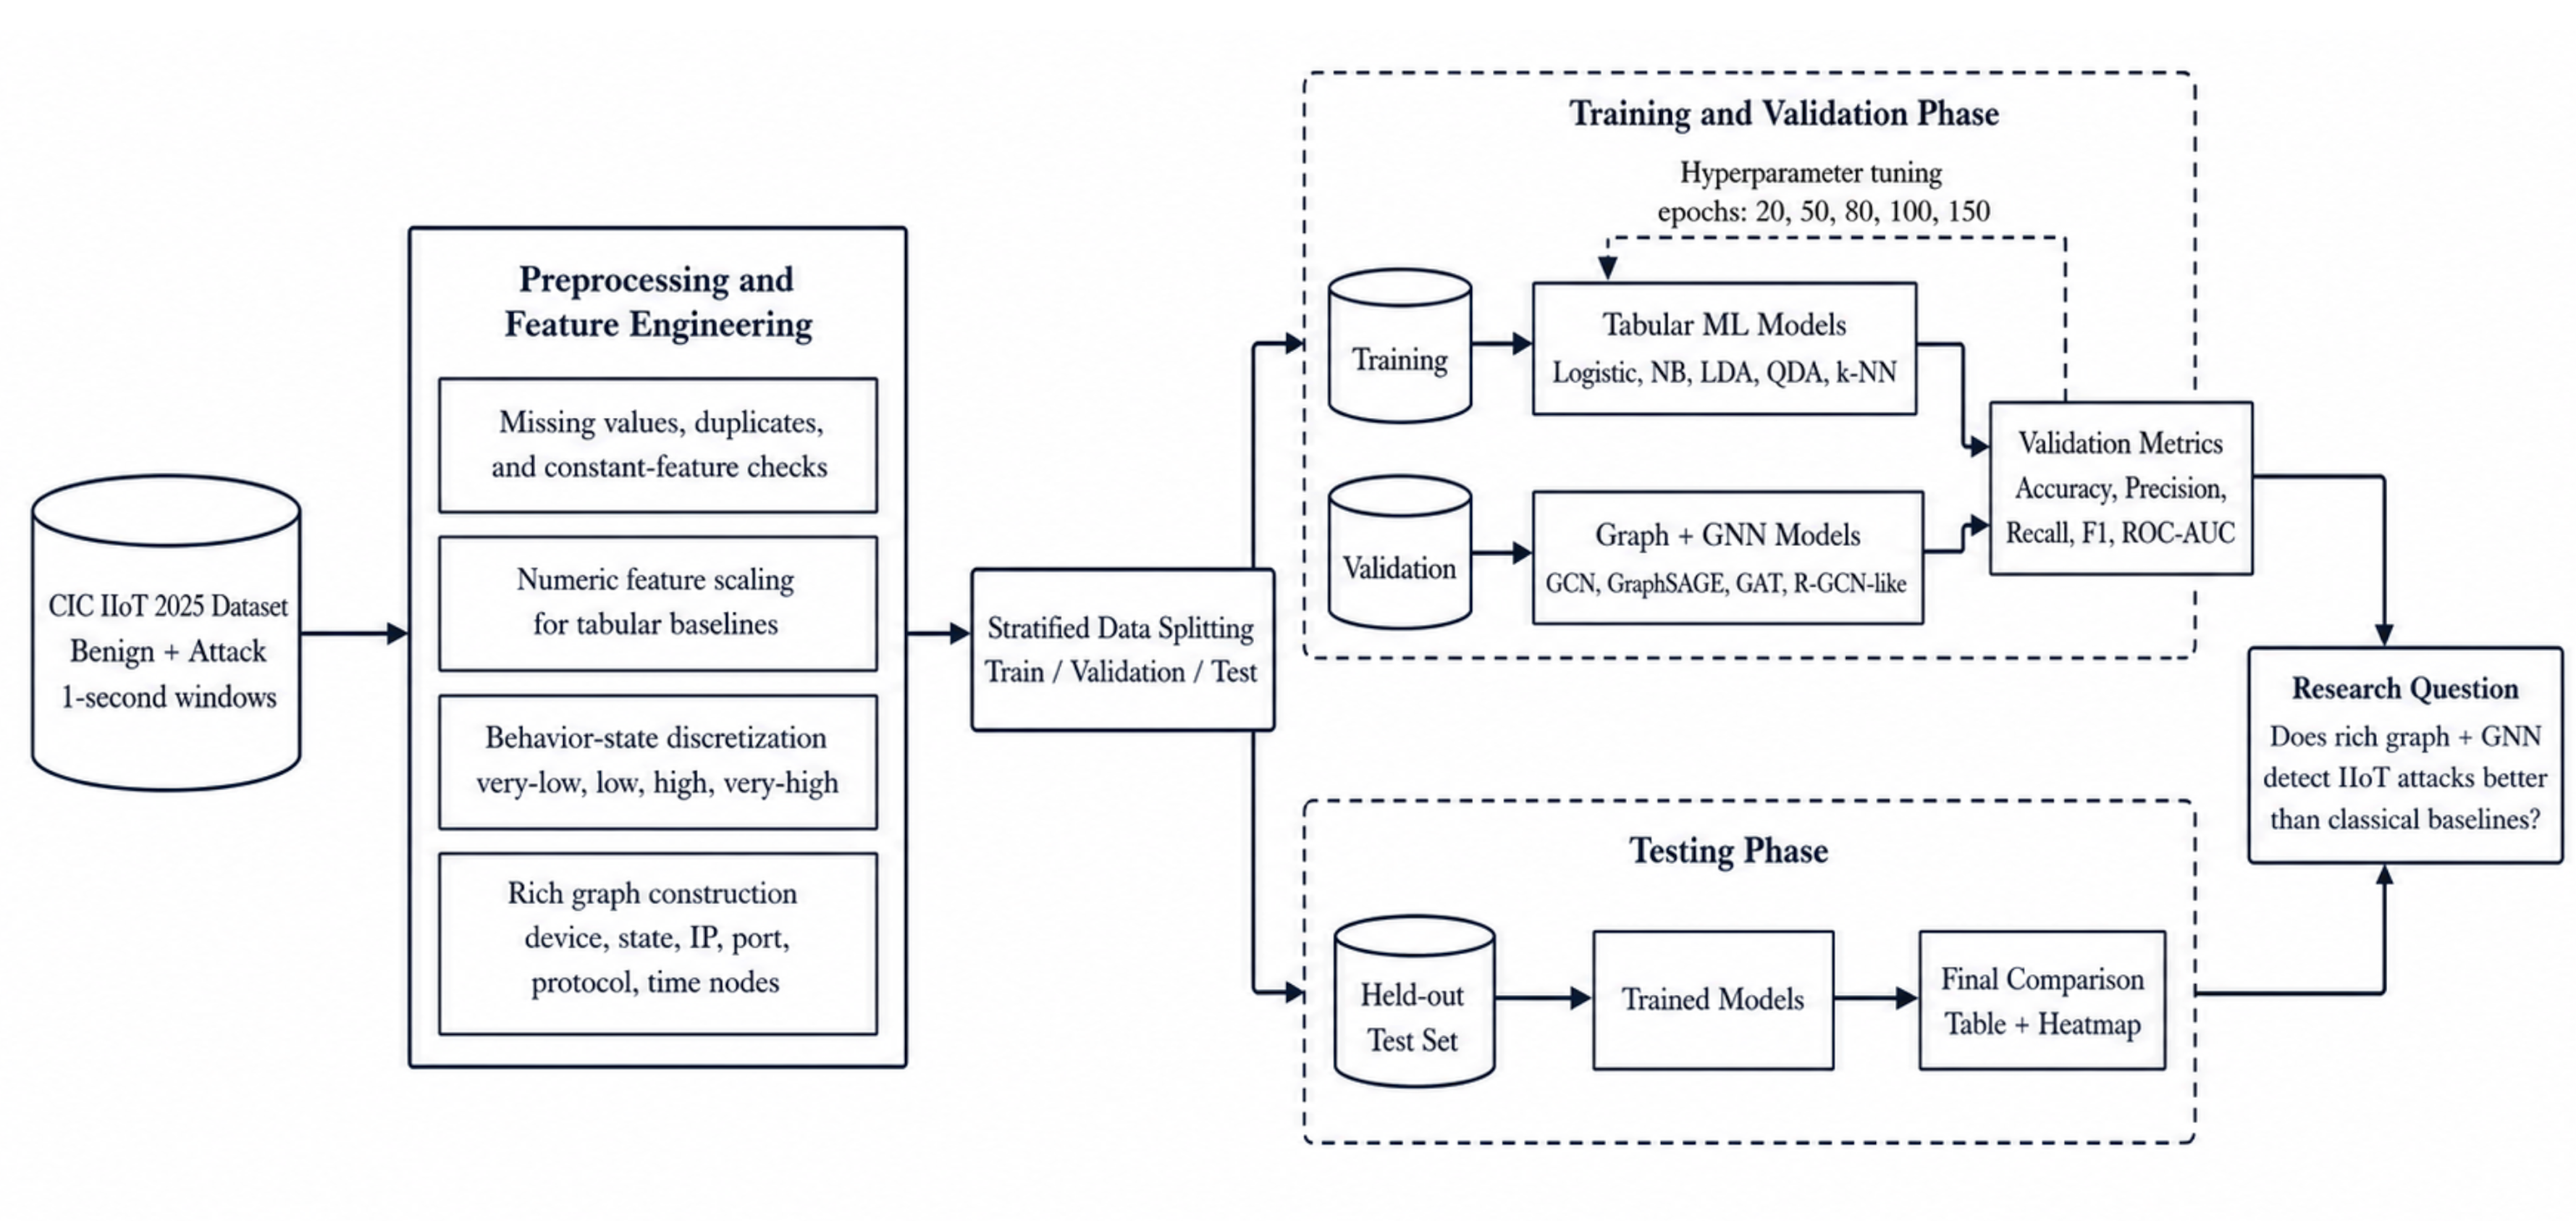
\includegraphics[width=\columnwidth]{figures/methodology.png}
    \caption{System model for IIoT intrusion detection using tabular baselines, Graph analysis and rich graphs GNNs - generated by Codex 5.5 \citep{openai_gpt54_2026}}
    \label{fig:meethodology}
\end{figure}

%Tabular classification methods
\subsection{Tabular classification methods}
\label{tabular classification methods}

The intrusion detection study performed in this paper is  a binary supervised classification problem. Each observation represents a 1-second network traffic window from the CIC IIoT 2025 dataset. The response variable is defined as:
\[
y_i =
\begin{cases}
0, & \text{benign traffic}, \\
1, & \text{attack traffic}.
\end{cases}
\]

Each row is represented as a feature vector:
\[
\mathbf{x}_i = (x_{i1}, x_{i2}, \ldots, x_{ip}),
\]
where $p$ is the number of selected traffic features after preprocessing.

The dataset was first divided using an 80/20 stratified train-test split. Then, 10-fold cross-validation was applied to the tabular baselines to preserve the benign/attack proportion across both sets. The training set was used to fit and apply some tweaks to the models and adjust thresholds when needed, the test set was used for final comparison with all the models. Moreover, 10-foldCV (k-fold cross validation technique) was applied to the tabular baselines to evaluate if model performance is stable across different training partitions.

We used an 80/20 stratified split with \texttt{random\_state = 42}.

\begin{table}[H]
\caption{Training and test split distribution.}
\centering
\small
\setlength{\tabcolsep}{4pt}
\renewcommand{\arraystretch}{1.15}
\resizebox{\columnwidth}{!}{%
\begin{tabular}{lrrrrr}
\toprule
\textbf{Split} & \textbf{Total Rows} & \textbf{Benign} & \textbf{Attack} & \textbf{Benign \%} & \textbf{Attack \%} \\
\midrule
Training set & 181,752 & 109,440 & 72,312 & 60.21\% & 39.79\% \\
Test set & 45,439 & 27,360 & 18,079 & 60.21\% & 39.79\% \\
\bottomrule
\end{tabular}
}
\label{tab:train_test_split_distribution}
\end{table}


Then we assessed the model using the parameters for classification for example: accuracy, precision, recall, F1-score, and ROC-AUC. In this study, recall and F1-score are especially important because missed attacks imply more money spent by companies when it comes to intrusion detection.


The evaluation metrics are defined as follows: we compare the models using the following evaluation metrics, which summarize different aspects of binary classification performance, including overall correctness, positive prediction quality, sensitivity to attacks, true negative performance, ranking ability, and probability calibration.

\begin{align}
\text{Accuracy} &= \frac{TP + TN}{TP + TN + FP + FN} \label{eq:accuracy} \\
\text{Precision} &= \frac{TP}{TP + FP} \label{eq:precision} \\
\text{Recall} &= \frac{TP}{TP + FN} \label{eq:recall} \\
\text{Specificity} &= \frac{TN}{TN + FP} \label{eq:specificity} \\
F_1\text{-score} &= 2 \times \frac{\text{Precision} \times \text{Recall}}{\text{Precision} + \text{Recall}} \label{eq:f1} \\
\text{ROC-AUC} &= \int_{0}^{1} TPR(FPR^{-1}(x))\,dx \label{eq:rocauc} \\
\text{Brier Score} &= \frac{1}{N}\sum_{i=1}^{N}(p_i - y_i)^2 \label{eq:brier}
\end{align}

where \(TP\) is true positives, \(TN\) is true negatives, \(FP\) is false positives, and \(FN\) is false negatives. In addition, \(TPR\) denotes the true positive rate, \(FPR\) denotes the false positive rate, \(p_i\) is the predicted probability for observation \(i\), \(y_i \in \{0,1\}\) is the true class label, and \(N\) is the total number of observations.

\subsubsection{Logistic Regression}

\cite{alma990016042380204808} says that Logistic Regression is the standard baseline for binary classification techniques. It estimates the probability that a window belongs to the attack class. The model is defined as:
\[
P(Y = 1 \mid \mathbf{x}) =
\frac{1}{1 + e^{-(\beta_0 + \beta_1x_1 + \cdots + \beta_px_p)}}
\]
where $\beta_0$ we know it as the intercept and $\beta_1, \ldots, \beta_p$ are the coefficients. Positive coefficients indicate features associated with higher attack probability and negative coefficients are features associated with benign behavior \citep{alma990016042380204808}.
\begin{figure}[htbp]
    \centering
    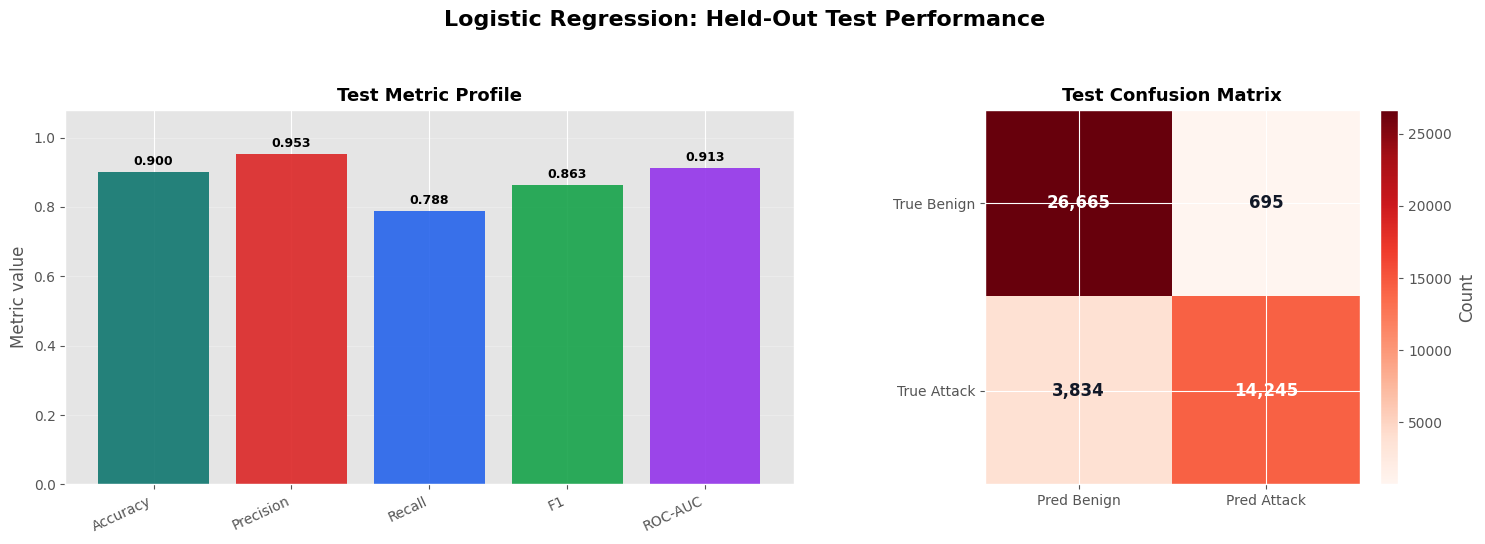
\includegraphics[width=0.95\columnwidth]{figures/baseline_logistic_regression_test_profile.png}
    \caption{Held-out test performance profile for Logistic Regression}
    \label{fig:logistic_regression_test_profile}
\end{figure}


\subsubsection{Naive Bayes}

Naive Bayes is used to estimate the probability of each class using Bayes theorem shown below, it assumes that predictors are conditionally independent given the class label:
\[
P(Y = k \mid \mathbf{x}) =
\frac{P(Y = k)P(\mathbf{x} \mid Y = k)}{P(\mathbf{x})}
\]
The naive assumption simplifies the likelihood as:
\[
P(\mathbf{x} \mid Y = k) =
\prod_{j=1}^{p} P(x_j \mid Y = k)
\]
Although this independence assumption is often unrealistic in network traffic, Naive Bayes provides a simple useful baseline \citep{alma990016042380204808,sahami1998bayesian}.
However, \citep{hocevar2025can} suggest that it may lag behind when the input distribution becomes more complex or adversarial, especially when dealing with AI-modified spam that significantly reduced its detection performance.
\begin{figure}[htbp]
    \centering
    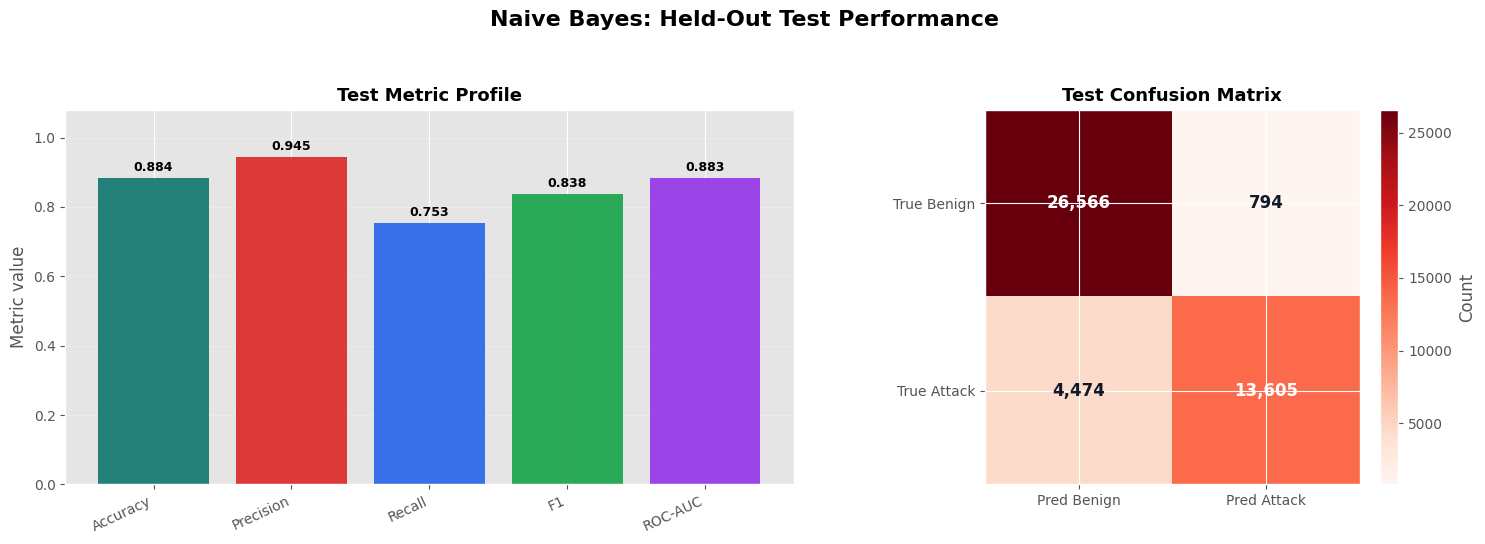
\includegraphics[width=0.95\columnwidth]{figures/baseline_naive_bayes_test_profile.png}
    \caption{Held-out test performance profile for Naive Bayes}
    \label{fig:naive_bayes_test_profile}
\end{figure}

\subsubsection{Linear Discriminant Analysis}

Fisher (1936, as cited in Mardia, Kent, \& Taylor, 2023, p.~2) \citep{mardia2023fisher} introduced Linear Discriminant Analysis or LDA technique in 1936. LDA assumes that each class follows a multivariate normal distribution and that the classes share the same covariance matrix. The general assumption is:
\[
\mathbf{x} \mid Y = k \sim N(\boldsymbol{\mu}_k, \boldsymbol{\Sigma})
\]
Because the covariance matrix is shared across classes, LDA produces a linear decision boundary.
\begin{figure}[htbp]
    \centering
    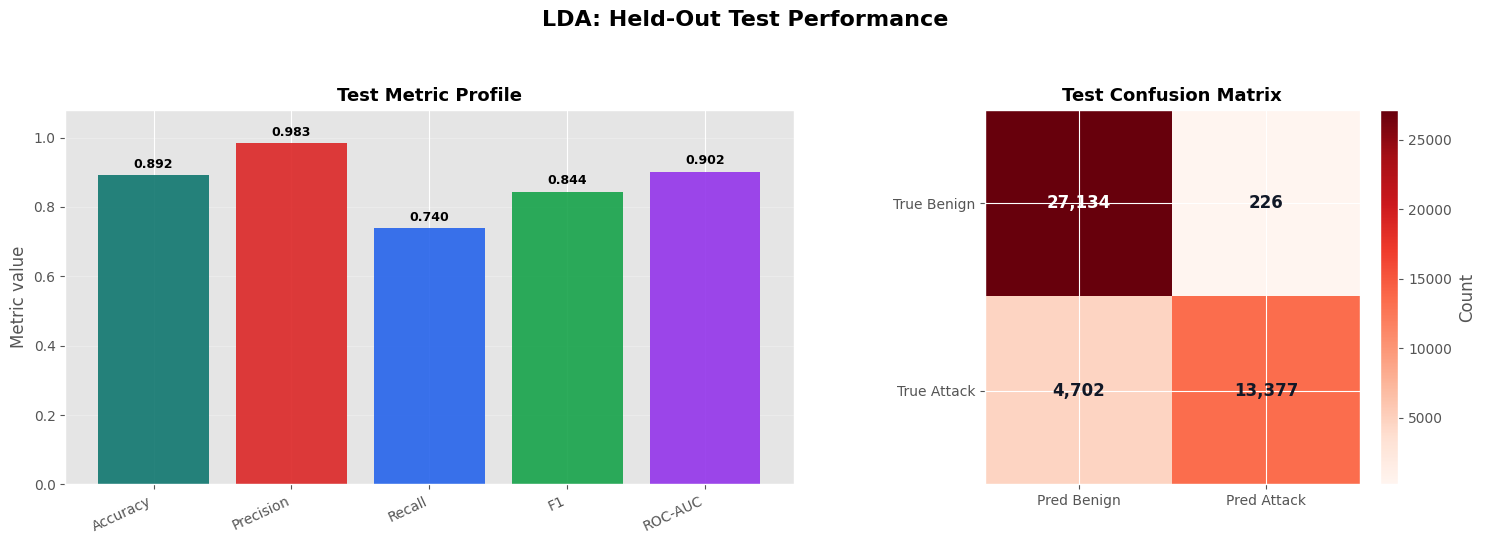
\includegraphics[width=0.95\columnwidth]{figures/baseline_lda_test_profile.png}
    \caption{Held-out test performance profile for LDA}
    \label{fig:lda_test_profile}
\end{figure}

\subsubsection{Quadratic Discriminant Analysis}

Quadratic Discriminant Analysis or QDA is similar to LDA, but it allows each class to have its own covariance matrix, that is the difference:
\[
\mathbf{x} \mid Y = k \sim N(\boldsymbol{\mu}_k, \boldsymbol{\Sigma}_k)
\]
The matrix can differ by class, that is why QDA creates a quadratic decision boundary. This makes QDA more flexible than LDA, it can also be more sensitive to noise, variance. \citep{alma990016042380204808}.

\begin{figure}[htbp]
    \centering
    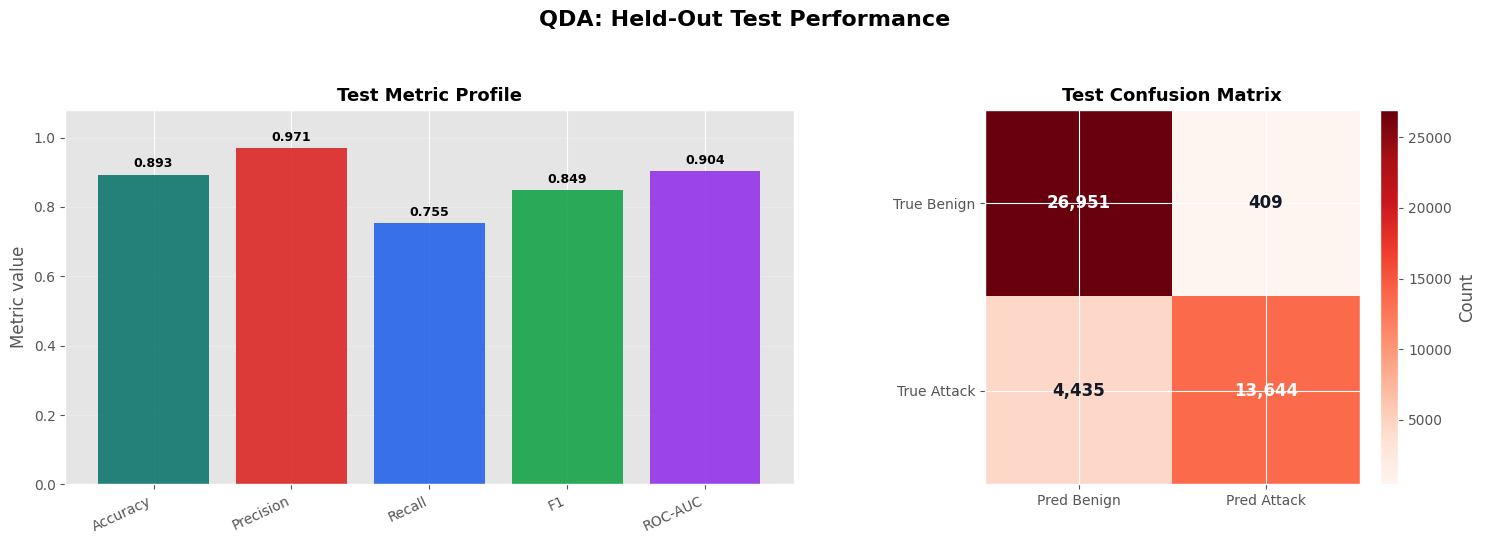
\includegraphics[width=0.95\columnwidth]{figures/baseline_qda_test_profile.png}
    \caption{Held-out test performance profile for QDA}
    \label{fig:qda_test_profile}
\end{figure}

\subsubsection{k-Nearest Neighbors}

The k-Nearest Neighbors classifier predicts the class of a new observation based on the majority class among its $k$ closest observations in the used training set. In this study, $k = 5$ was set as the baseline.
\[
\hat{y}_i =
\text{majority vote among the } k \text{ nearest neighbors of } \mathbf{x}_i
\]
k-NN does not assume a specific functional form, it classifies attack and benign windows based on similarity to neighbors \citep{alma990016042380204808, alharthi2025comparative}.

\begin{figure}[htbp]
    \centering
    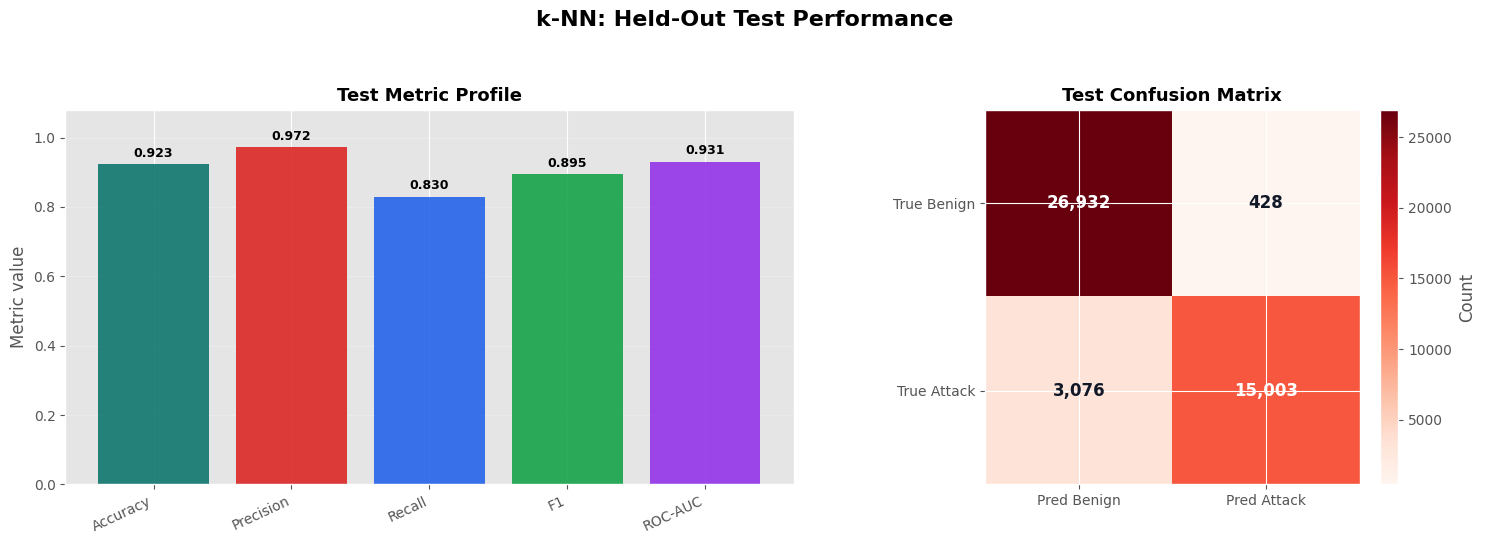
\includegraphics[width=0.95\columnwidth]{figures/baseline_knn_test_profile.png}
    \caption{Held-out test performance profile for k-NN}
    \label{fig:knn_test_profile}
\end{figure}

%Graphs Designs
\begingroup
\color{red}
\subsection{Graph Analysis Designs}
\label{sec:graph_analysis_designs}

This stage, in which we performed three different graph analysis, was conducted to test whether the relationships in the traffic data were meaningful to answering our research question and as a preliminary step before applying a GNN. Instead of treating each row as a flat vector, the graphs represent devices and traffic states as connected entities. Graphs offer a richer universal representation that offers a sophisticated perspective of a system. 

Unlike flat data (records in a table or in a .csv file), which strips away the relational context losing the big picture, graph capture the deep context necessary to detect anomaly behavior, as most intrusions consist of a specific interaction between host and processes; using a relational graph makes it easier to capture these patterns \citep{bilot2023graph, jiang2019anomaly}. A graph is simply represented as
\[
G = (V, E)
\]
where \(V\) is a set of nodes (or entities) and \(E\) is a set of edges (or relations) between those nodes.

\citep{bilot2023graph} indicate that graphs representation involves extracting informative features, they referred to this as \textit{``embeddings''} from a graph. It is possible to capture different information into embeddings. Therefore, the first graph representation used in this study was a device-to-behavior-state graph. We decided to make it this way, to evaluate graph initial performance, IIoT devices were represented as device nodes, while selected numerical traffic features were discretized into behavior-state nodes such as low packet count, high port diversity, or high IP-length values. The edges connected each device to the behavior states observed in its 1-second traffic windows. This representation was used for the initial graph-analysis methods and for the first simple GCN model. This creates a bipartite graph. A bipartite graph has two types of nodes and edges only across the two groups. Here the devices are in one group and behavior are the other.
\[
\text{device node} \rightarrow \text{behavior-state nodes}
\]

\begin{table}[H]
\caption{Example flat IIoT record used to build the simple device-to-behavior-state graph.}
\centering
\small
\setlength{\tabcolsep}{5pt}
\renewcommand{\arraystretch}{1.15}
\begin{tabular}{llll}
\hline
\textbf{device\_name} & \textbf{packets\_state} & \textbf{ports\_state} & \textbf{ips\_state} \\ \hline
mqtt-broker & high & very-high & high \\ \hline
\end{tabular}
\label{tab:simple_device_state_record}
\end{table}

Table~\ref{tab:simple_device_state_record} can be represented as a graph in which the device is modeled as the central node and its related traffic attributes are modeled as connected nodes \citep{noble2003graph}. This representation transforms a single 1-second traffic window from a flat tabular record (a table row) into a relational structure that includes source IPs, destination IPs, packet count, destination ports, and protocols.

\begin{figure}[H]
    \centering
    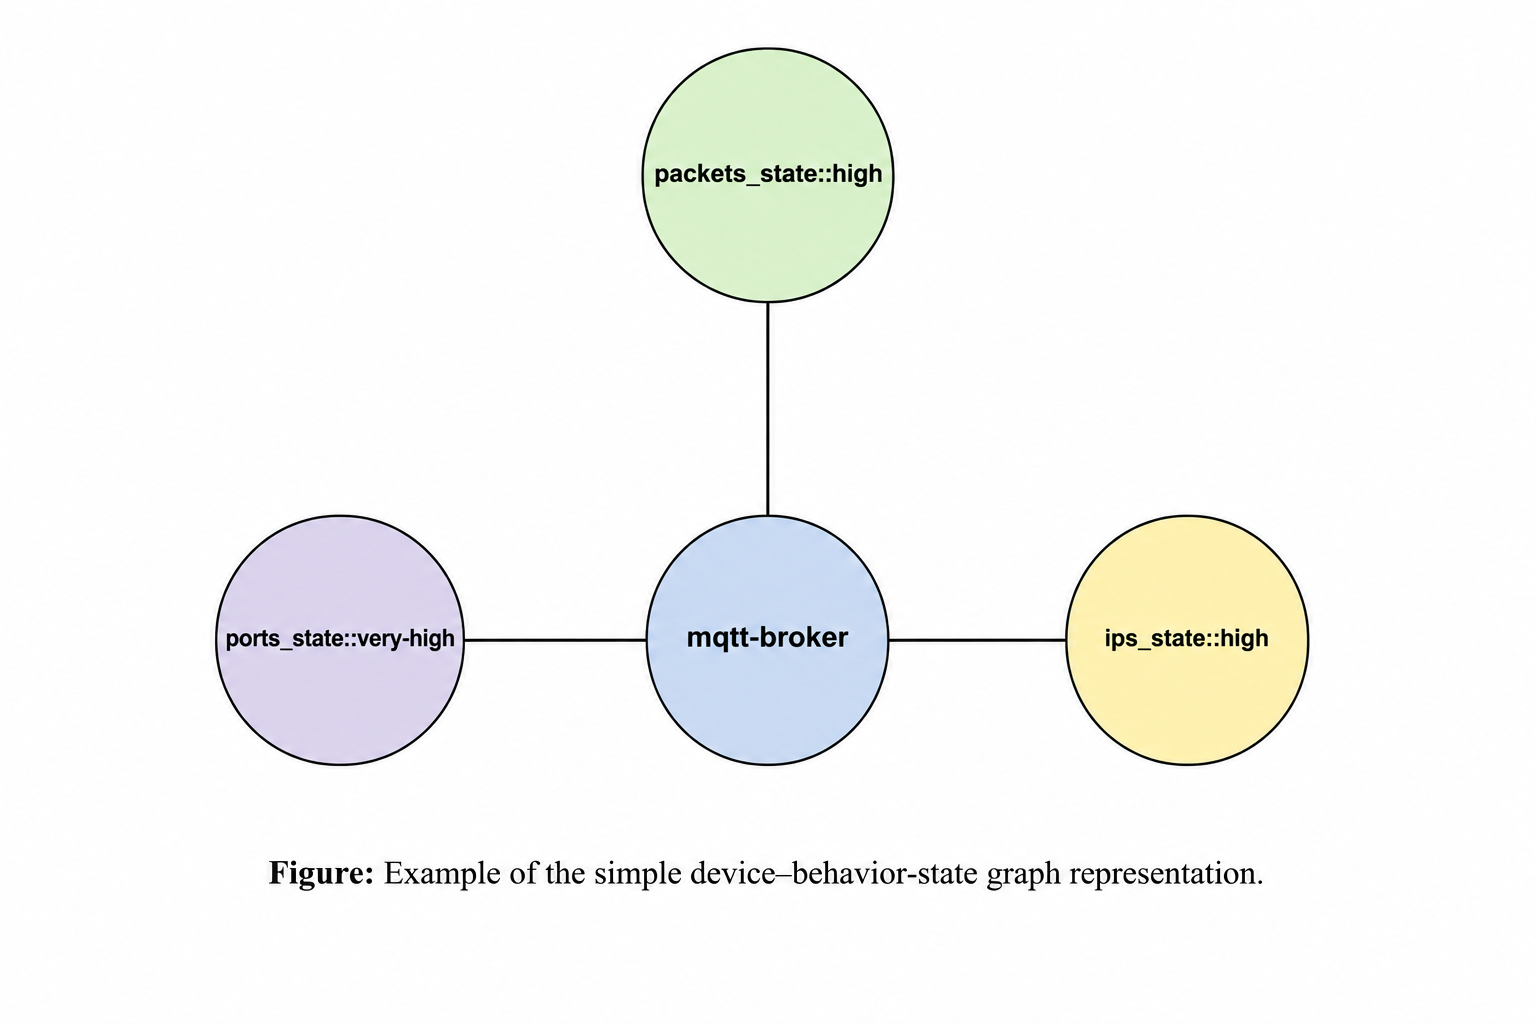
\includegraphics[width=\columnwidth]{figures/graph_record_example.png}
    \caption{Graphical representation of one IIoT traffic window as a device-centered graph -  generated by Codex 5.5 \citep{openai_gpt54_2026}.}
    \label{fig:graph_record_example}
\end{figure}

In this representation \ref{fig:device node -> behavior-state nodes}, we can visualize the devices as nodes connected the behavior-states such as ports of destination (ports\_dst), length of the IP (ip\_length), packet count (packets\_all) and others. They are categorized as very low, low, high, and very high.
\begin{figure}[H]
    \centering
    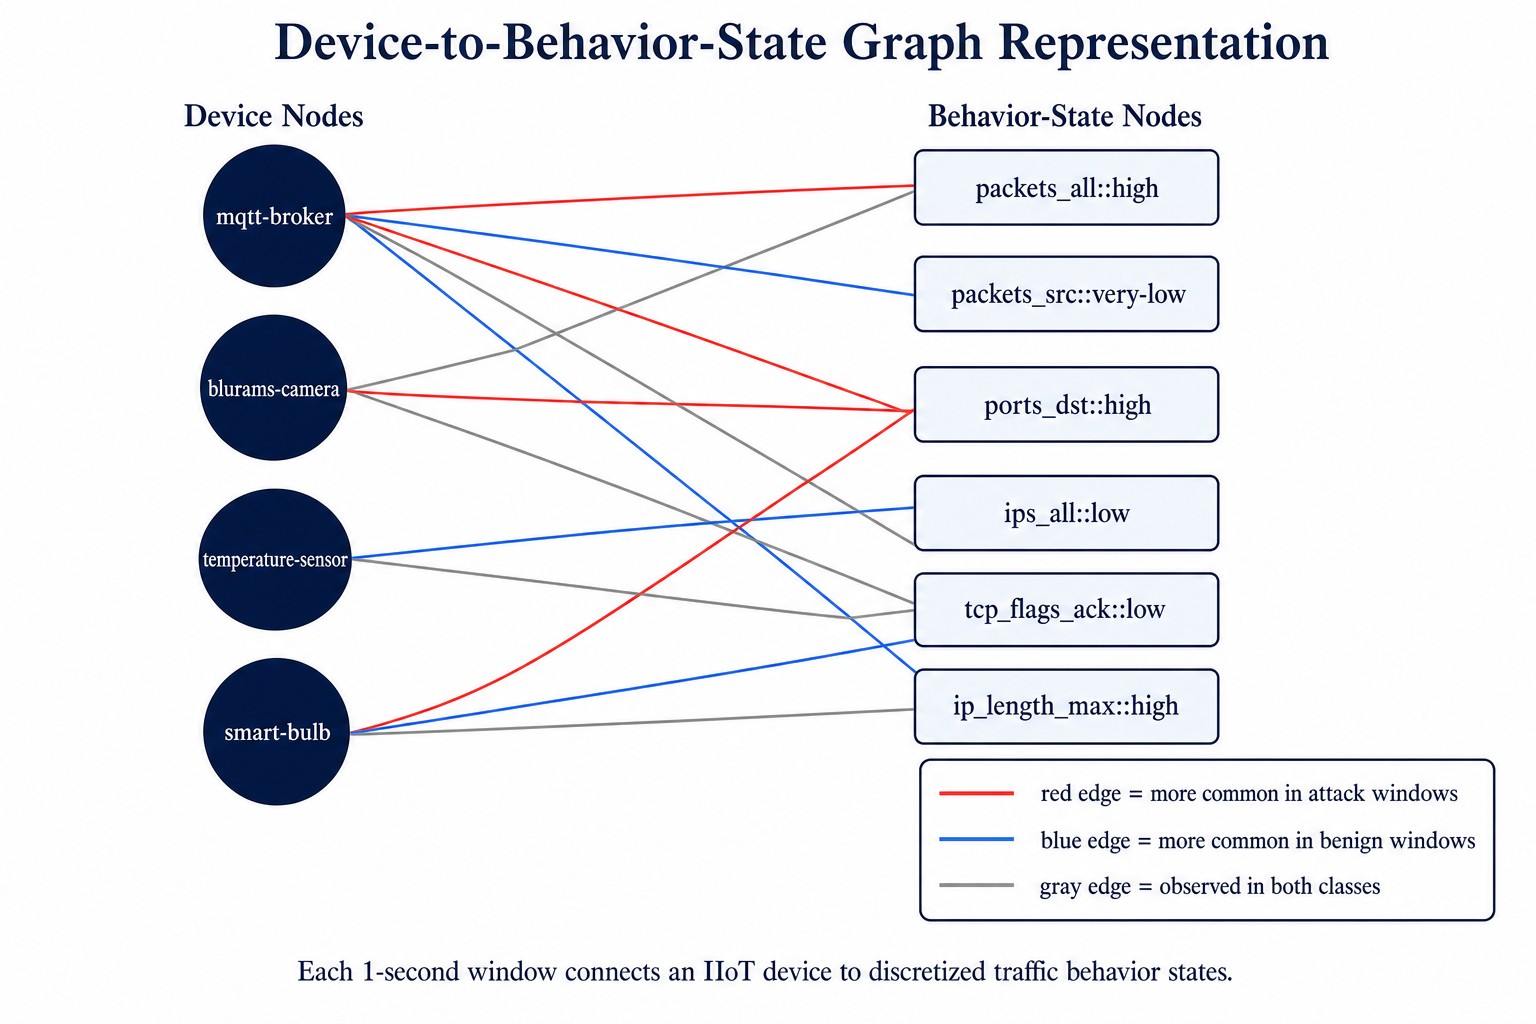
\includegraphics[width=\columnwidth]{figures/device_behavior_state_graph.png}
    \caption{Example of device-state graph representation}
    \label{fig:device node -> behavior-state nodes}
\end{figure}

\cite{jiang2019anomaly} explain that a problem with many anomaly detection models is that they only consider individual entity properties, which can lead to more false positives. They argue that the connections or relationships between entities should also be taken into account, therefore using Graphs and GNN can be useful tools for anomaly detection.

\subsubsection{Graph 1: Benign Novelty Graph}

The first graph method used is benign traffic, which is our reference model. We believed is that attack windows may contain device-state relationships that were not commonly observed during benign behavior. The idea is to learn normal patterns and flag as suspicious anything that rarely or never occurs in benign behavior. \cite{noble2003graph} mention that there is not a formal definition of what an anomaly detection means, but in their work they refer to it as a surprising event or an unusual occurrence. In our study, we are using a labeled dataset containing benign and attack behavior, for this initial graph we will use only the benign dataset as heuristic to capture unusual or different behavior that do not look benign. This method relates to anomaly detection techniques; it asks whether the pattern is unusual compared with benign behavior. 

% INSERT GRAPH 1 FIGURE HERE:
\begin{figure}[H]
    \centering
    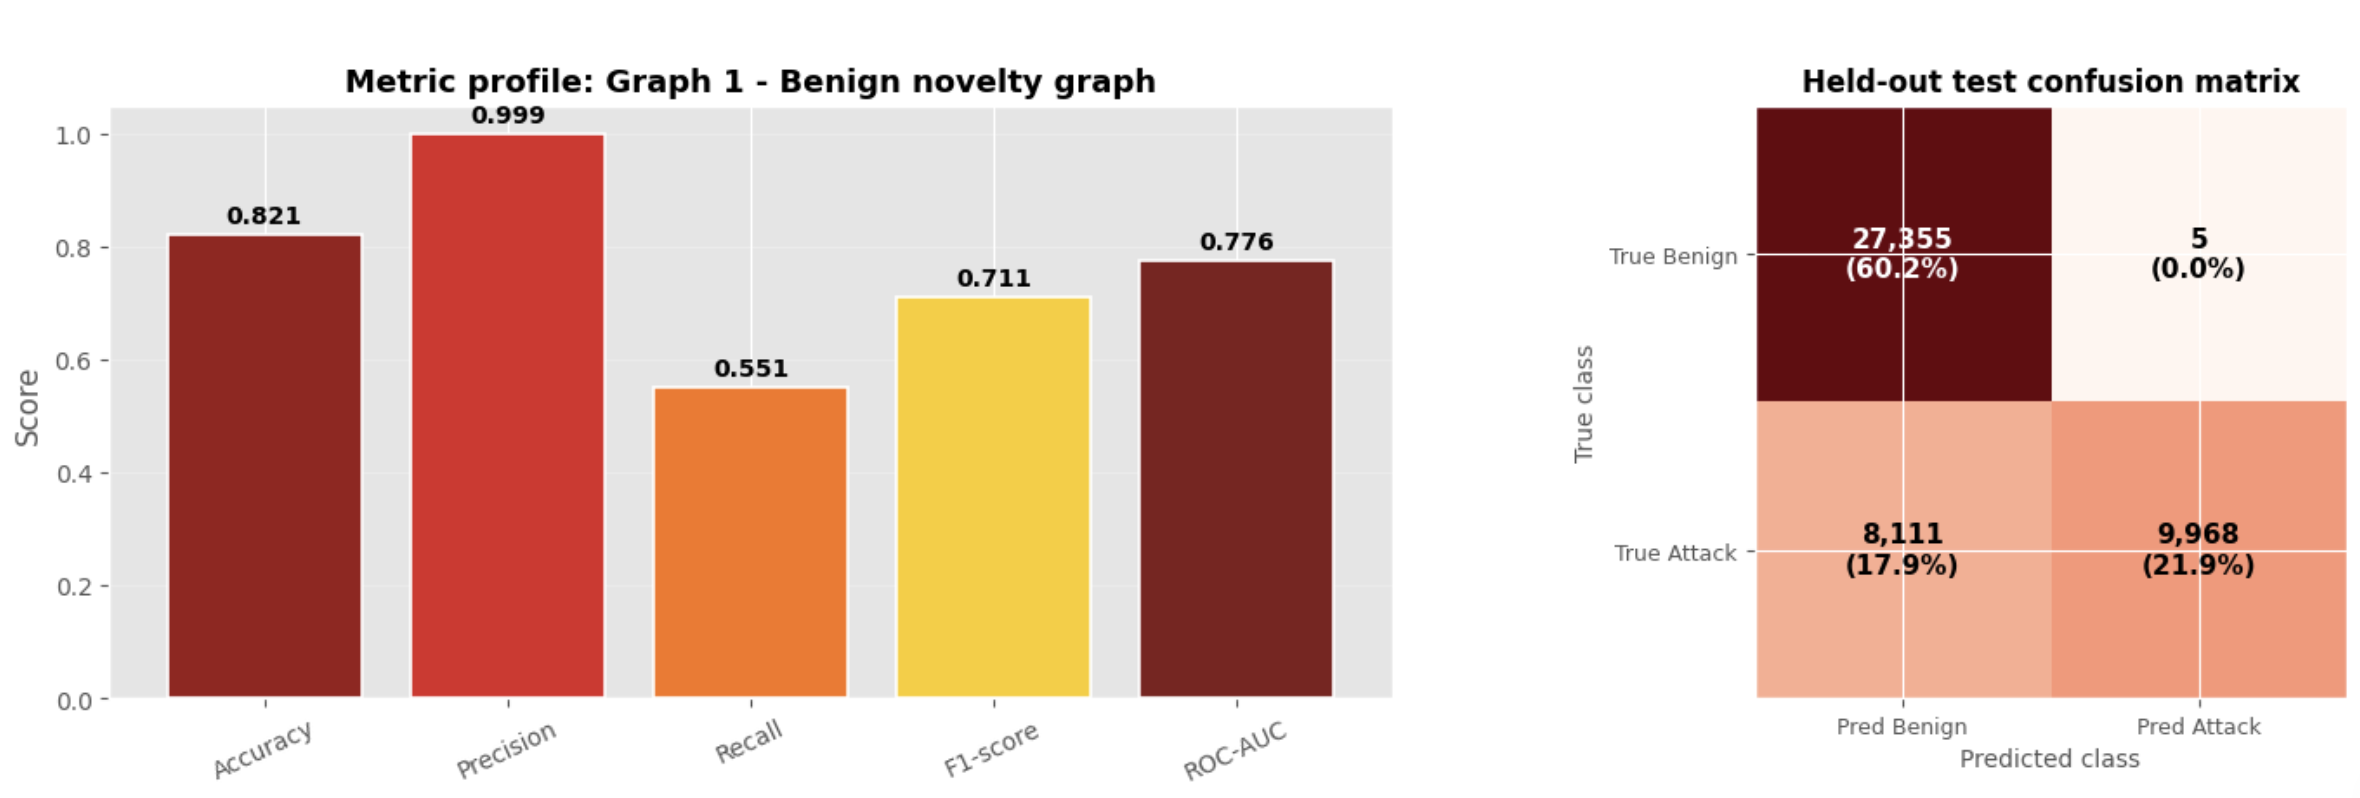
\includegraphics[width=\columnwidth]{figures/graph1.png}
    \caption{Held-out test performance of the Benign Novelty Graph, including evaluation metrics and confusion matrix}
    \label{fig:graph1_benign_novelty_results}
\end{figure}

\subsubsection{Graph 2: Dual-Class Affinity Graph}

The second graph method compares each device-state relationship against both benign and attack training patterns. 

We ask the following question: 
\begin{center}
\textbf{do this window's device-to-state edges look more like the attack graph or the benign graph?}
\end{center}
 In this heuristic, we now use both datasets benign and attack. In Graph 1 figure ~\ref{fig:graph1_benign_novelty_results}, we only considered the benign dataset and sought for outliers in it to classify it as attack behavior. In a few words, this method is more balanced than the pure novelty detection we did previously. To do this, we use the same graph model \texttt{deviceName -> behaviorState}, for example:

\begin{center}
\texttt{mqtt-broker} \(\rightarrow\) \texttt{network\_packets\_all\_count::high}

\texttt{mqtt-broker} \(\rightarrow\) \texttt{network\_ports\_dst\_count::very-high}
\end{center}

An affinity score is computed by comparing attack support and benign support with the following scoring formula:

Let \(a_e\) be the attack edge count and \(b_e\) be the benign edge count. The dual affinity score is defined as:

\[
S_{\mathrm{dual}}
=
\overline{\log(1+a_e)}
-
\overline{\log(1+b_e)}
\]

We define \texttt{attack\_edge\_count} as the number of times the connection appears in attack windows, and \texttt{benign\_edge\_count} as the number of times it appears in benign windows, which we define as normal behavior. We computed the Affinity-class for every 1-second window using the training set. The threshold was calculated using the F1 score, testing various possible thresholds, and the resulting threshold that gave us the best overall result was 0.044.
\[
\begin{cases}
\text{score} \geq 0.044 & \rightarrow \text{attack} \\
\text{score} < 0.044 & \rightarrow \text{benign}
\end{cases}
\]

If the resulting score is high, it indicates more attack-like behavior; A positive score indicates that the window is more structurally similar to attack traffic, while a negative score indicates stronger similarity to benign traffic.

\begin{figure}[H]
    \centering
    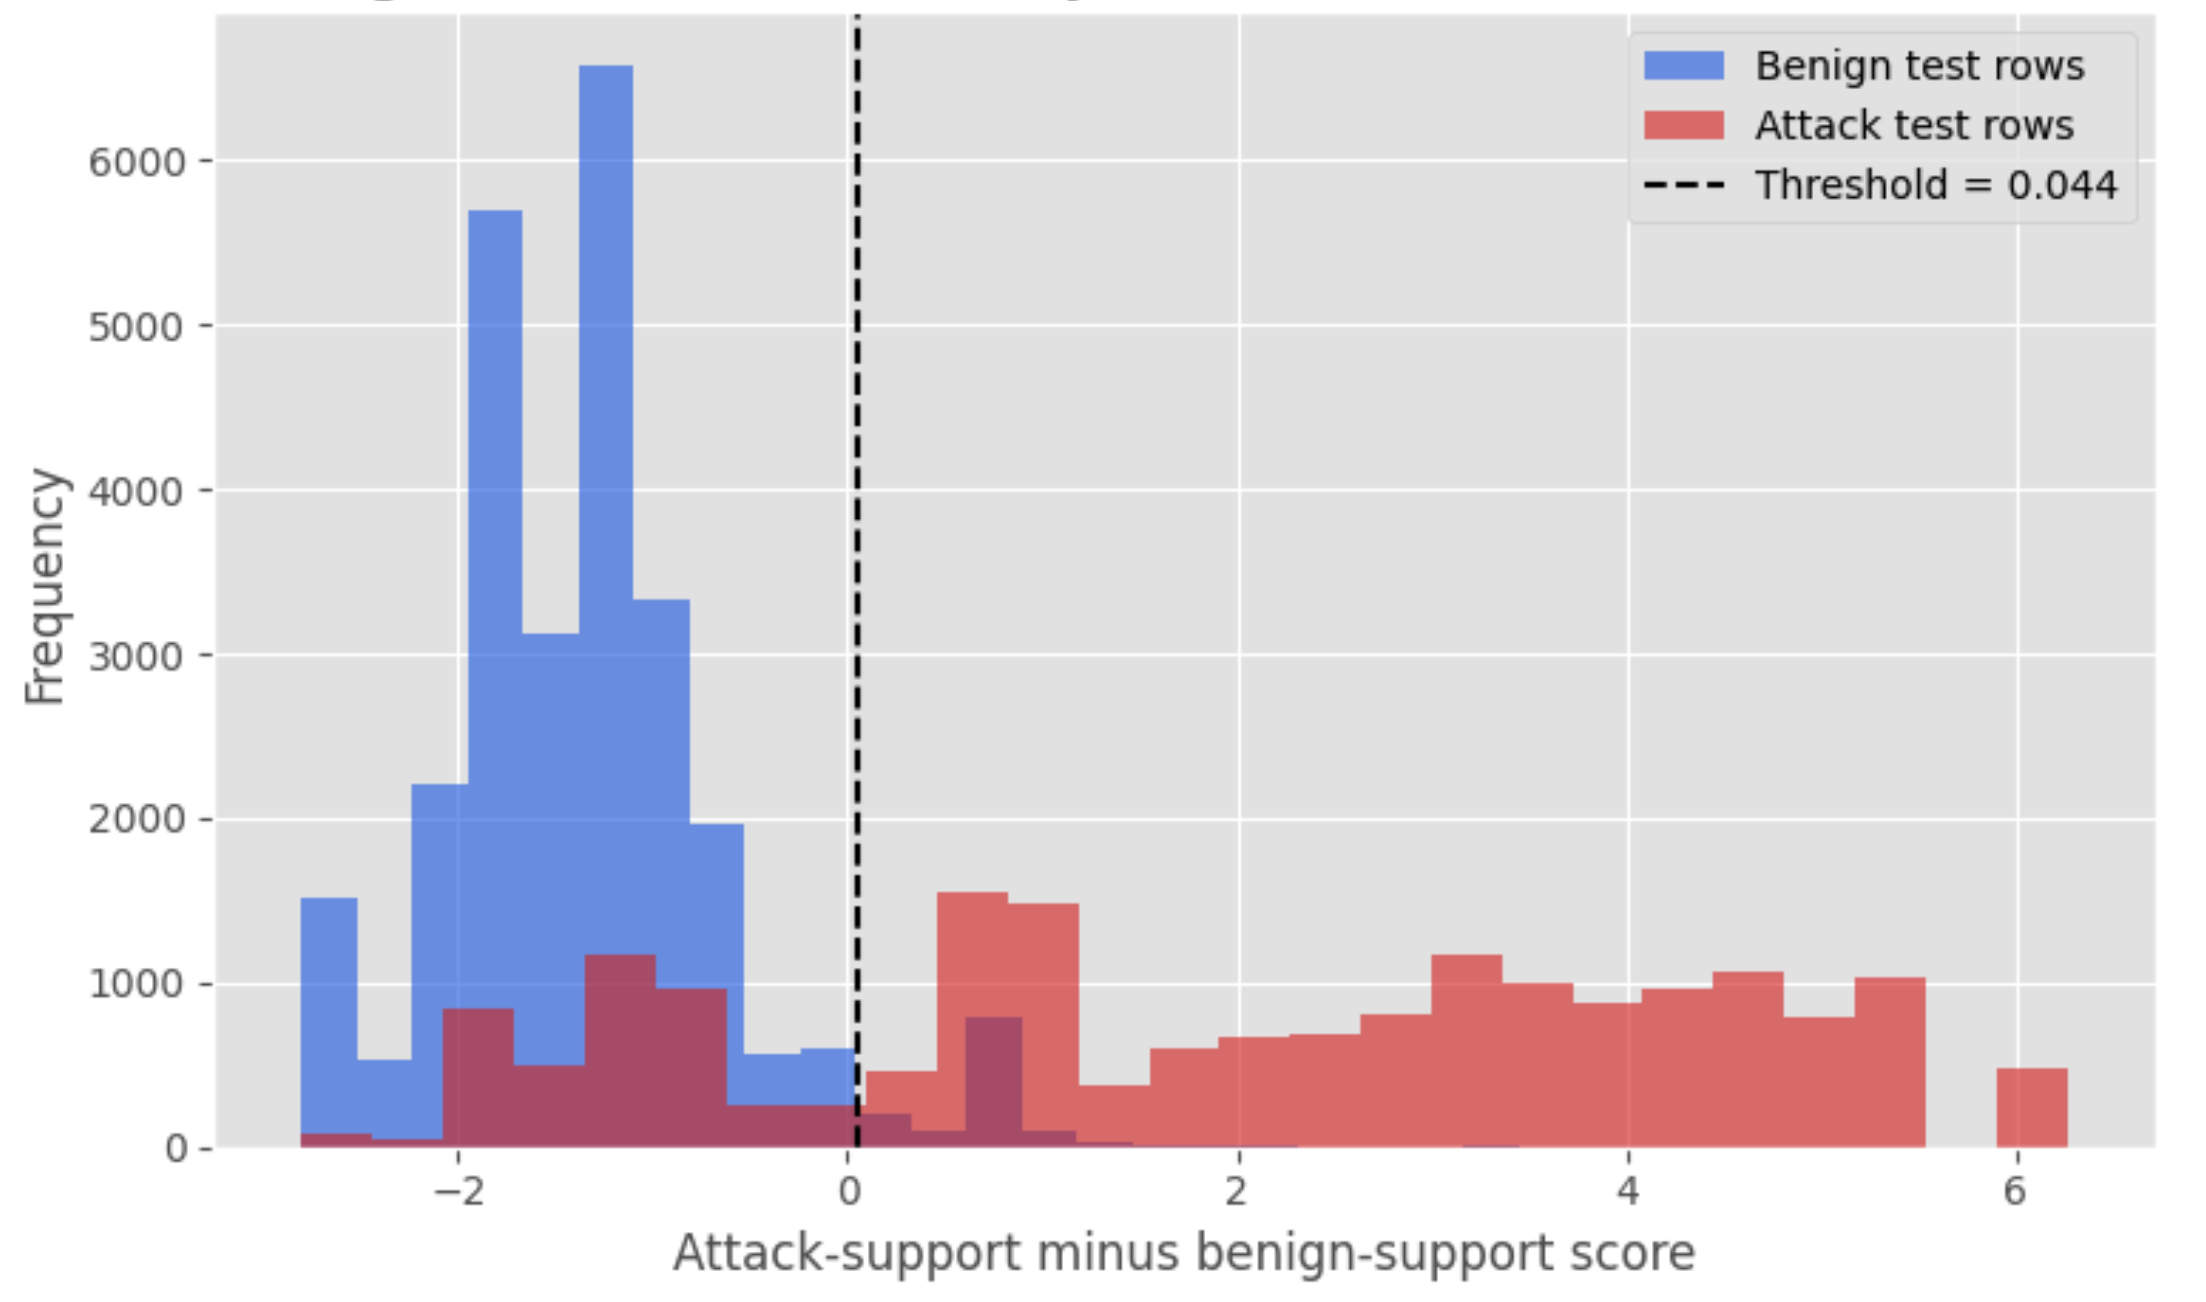
\includegraphics[width=\columnwidth]{figures/attack_benign_scoring.png}
    \caption{Dual-class affinity score distribution on the test set}
    \label{Dual-class affinity score distribution on the test set}
\end{figure}

After applying the dual-class affinity scoring function to the held-out test set, the results are shown in figure \ref{fig:graph2_affinity-class_results}
\begin{figure}[H]
    \centering
    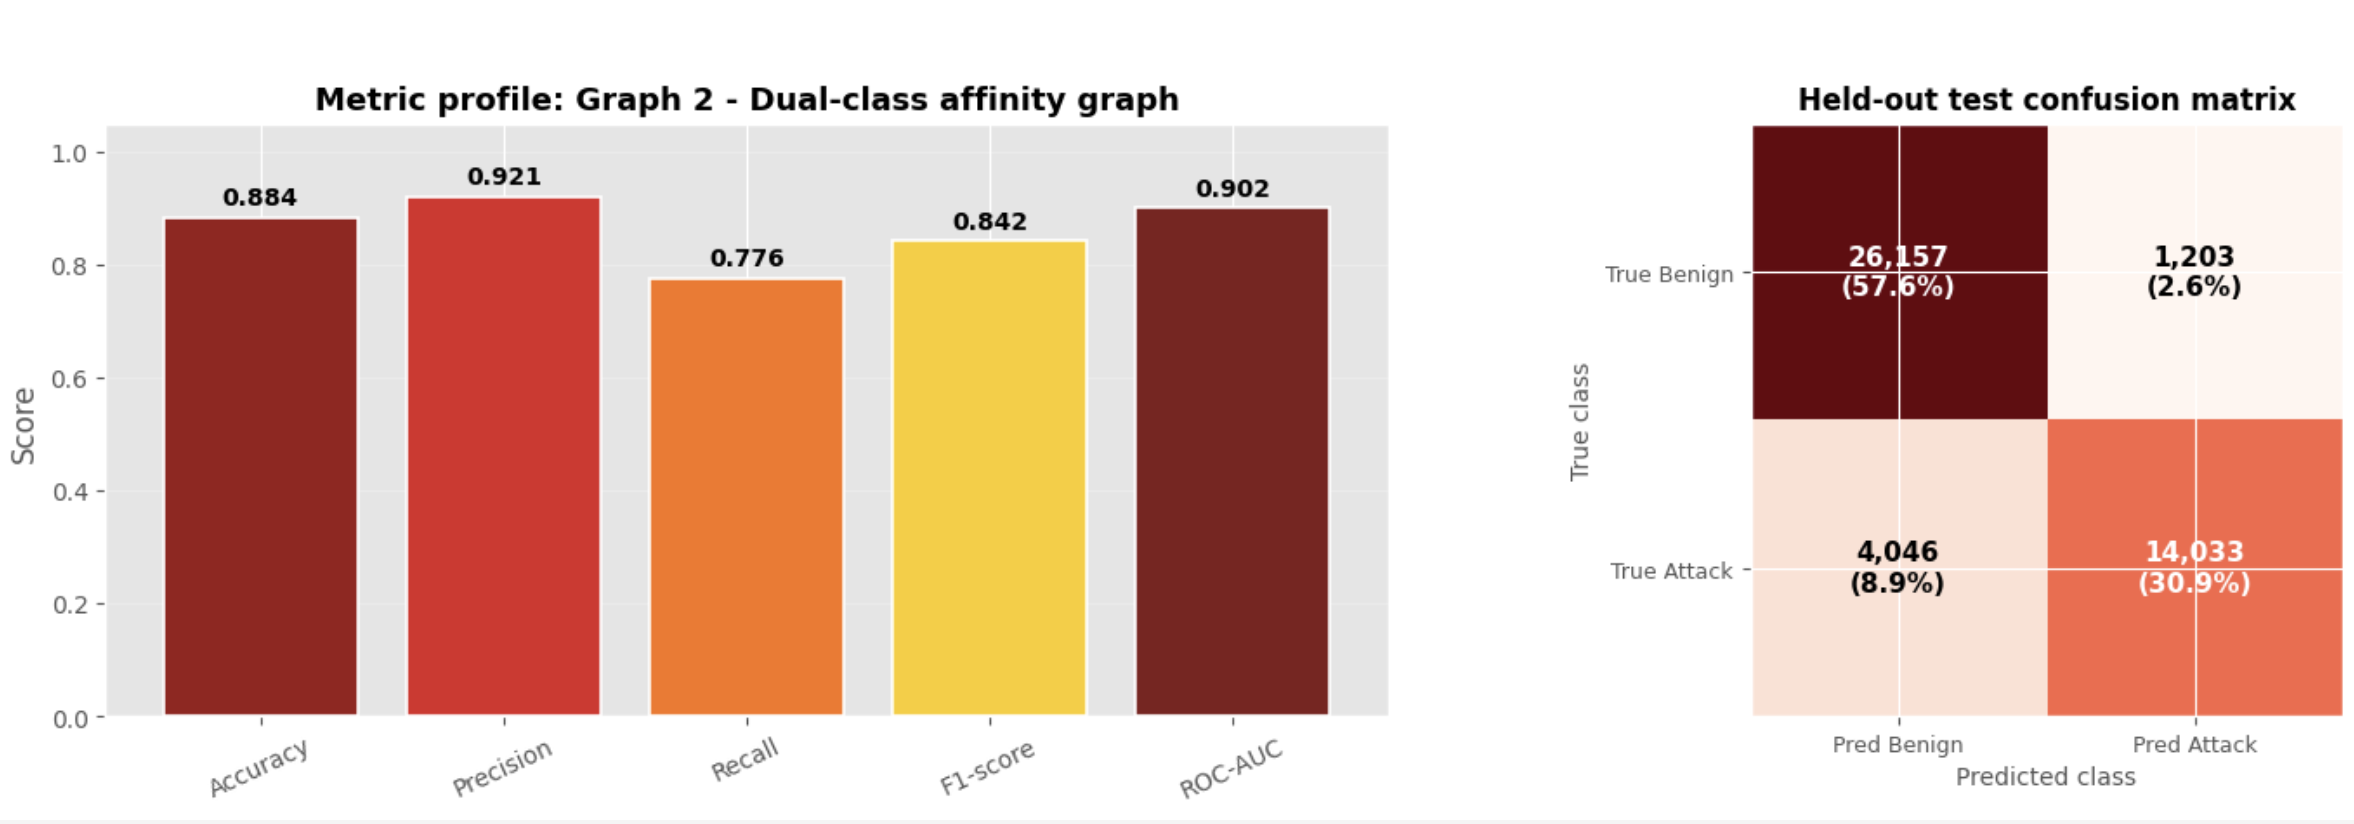
\includegraphics[width=\columnwidth]{figures/graph2.png}
    \caption{Held-out test performance of the dual-class affinity graph, including evaluation metrics and confusion matrix}
    \label{fig:graph2_affinity-class_results}
\end{figure}

\subsubsection{Graph 3: State Co-occurrence Graph}

The third graph method focuses on combinations of traffic states. Some attacks may not be identified by a single feature but by how multiple feature states co-occur. An example is a high packet count combined with high port activity; it can be more suspicious than either feature alone. As we did in Novelty Graph \ref{fig:graph1_benign_novelty_results} and Dual-class Affinity Graph \ref{fig:graph2_affinity-class_results}, we use the \texttt{deviceName -> behaviorState} structure. We look at which states appear together within the same 1-second window.

For example, if we see a row with the following:

\begin{center}
\texttt{network\_packets\_all\_count::high}\\
\texttt{network\_ports\_dst\_count::very-high}\\
\texttt{network\_ips\_all\_count::high}\\
\texttt{network\_tcp-flags-ack\_count::low}
\end{center}

We ask:

\begin{center}
\textbf{Does this combination of states occur more frequently in benign traffic or in attack traffic?}
\end{center}

The threshold was calculated the same way as in Graph 2 as shown in figure \ref{Dual-class affinity score distribution on the test set}, using the training set that yielded the best F1 score. We test various possible thresholds using the existing scores. We chose the threshold that best balanced precision, recall, and F1 score. The resulting threshold was -0.082.

\[
\begin{cases}
\text{score} \geq -0.082 & \rightarrow \text{attack} \\
\text{score} < -0.082 & \rightarrow \text{benign}
\end{cases}
\]

The logic was as follows:

\begin{enumerate}
    \item We used the converted the numerical variables to very low, low, high, and very high as we did.
    \item For each window, we took the resulting states.
    \item We created pairs of states that appear together within that same window.
    \item We counted how many times each pair appeared in the benign and attack categories.
    \item We calculated a score by comparing support for the attack to support for the benign.
    \item If the score exceeds a threshold (-0.082), we classify the window as an attack.
    \item We use the following formula:
\end{enumerate}

Let \(a_p\) be the attack pair count, \(b_p\) be the benign pair count, and \(P_w\) be the set of co-occurring state pairs in a given 1-second window. The co-occurrence score is defined as:

\[
S_{\mathrm{co}}
=
\frac{1}{|P_w|}
\sum_{p \in P_w}
\left[
\log(1+a_p) - \log(1+b_p)
\right]
\]

\begin{figure}[H]
    \centering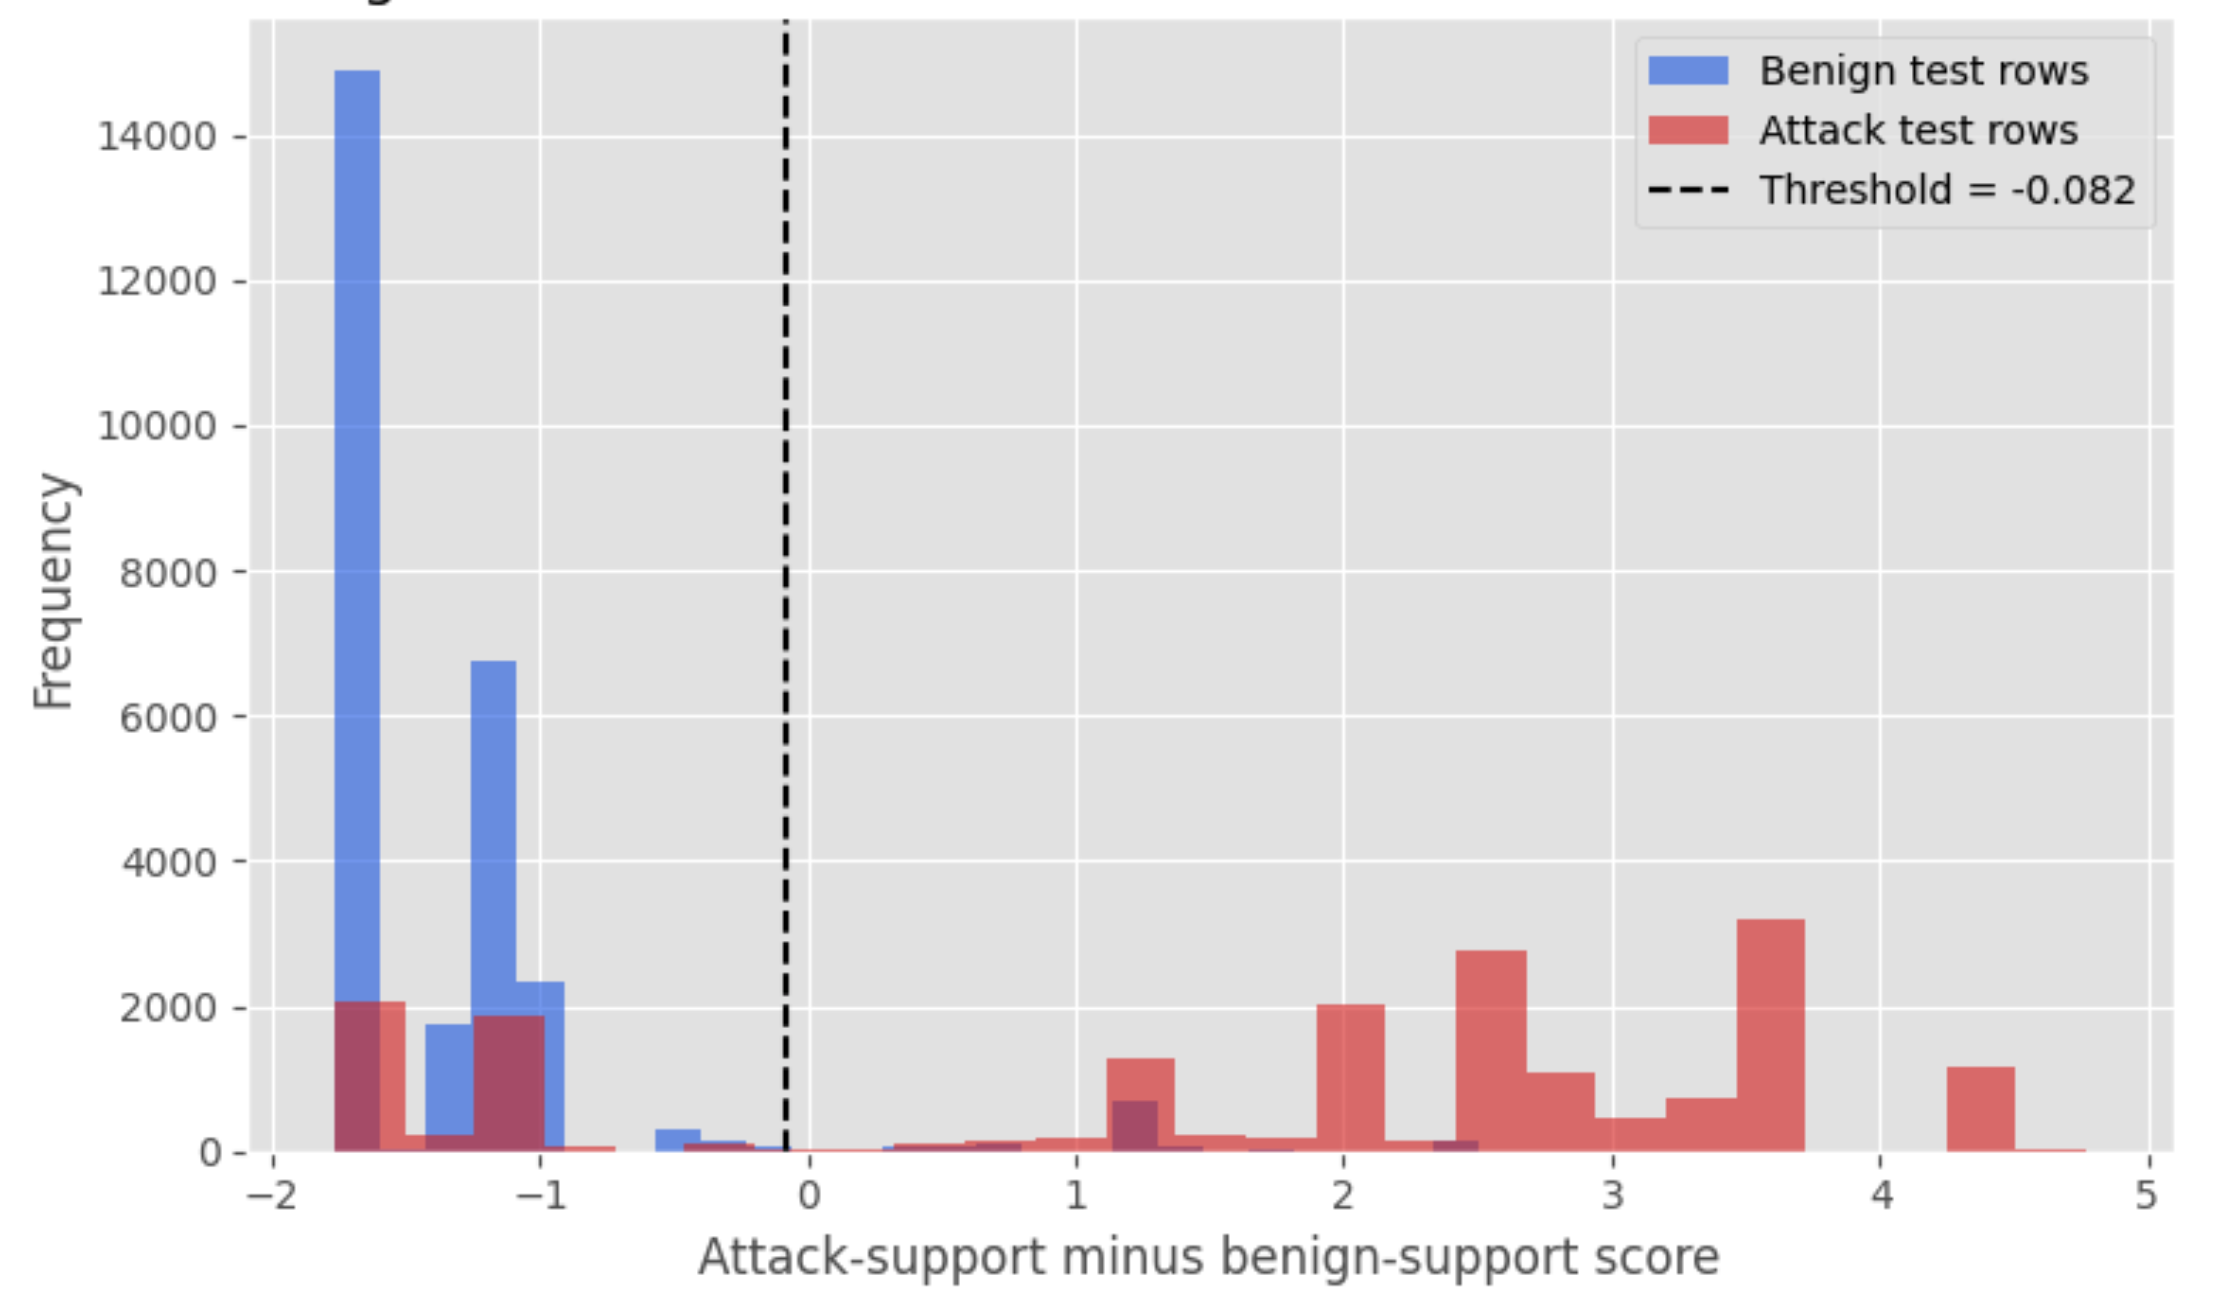
\includegraphics[width=\columnwidth]{figures/attack_benign_scoring_graph3.png}
    \caption{State co-occurence score distribution on the test set}
    \label{fig:State co-occurence score distribution on the test set}
\end{figure}





 The main idea is that an attack behavior is not always identifiable by a single isolated variable, but rather by a combination of signals. We aim to capture a combination of states that deviate from normal behavior. That aligns with the work of \cite{akoglu2015graph} regarding how to spot anomalies in the entire graph's structure by analyzing its nodes, edges, and subgraphs. For \cite{akoglu2015graph}, anomaly detection is often relational and can capture real-world phenomena. It is possible to have a richer graph representation in which nodes and edges exhibit different attributes. For example, in our study, many packets, many destination ports, many IPs, many source IPs, and many protocols can be suspicious, rather than just many packets alone.

After computing the results for the State co-occurrence graph, we obtain the following results shown in  figure \ref{fig:Graph 3 - Results and Confusion matrix Co-occurrence graph}
\begin{figure}[H]
    \centering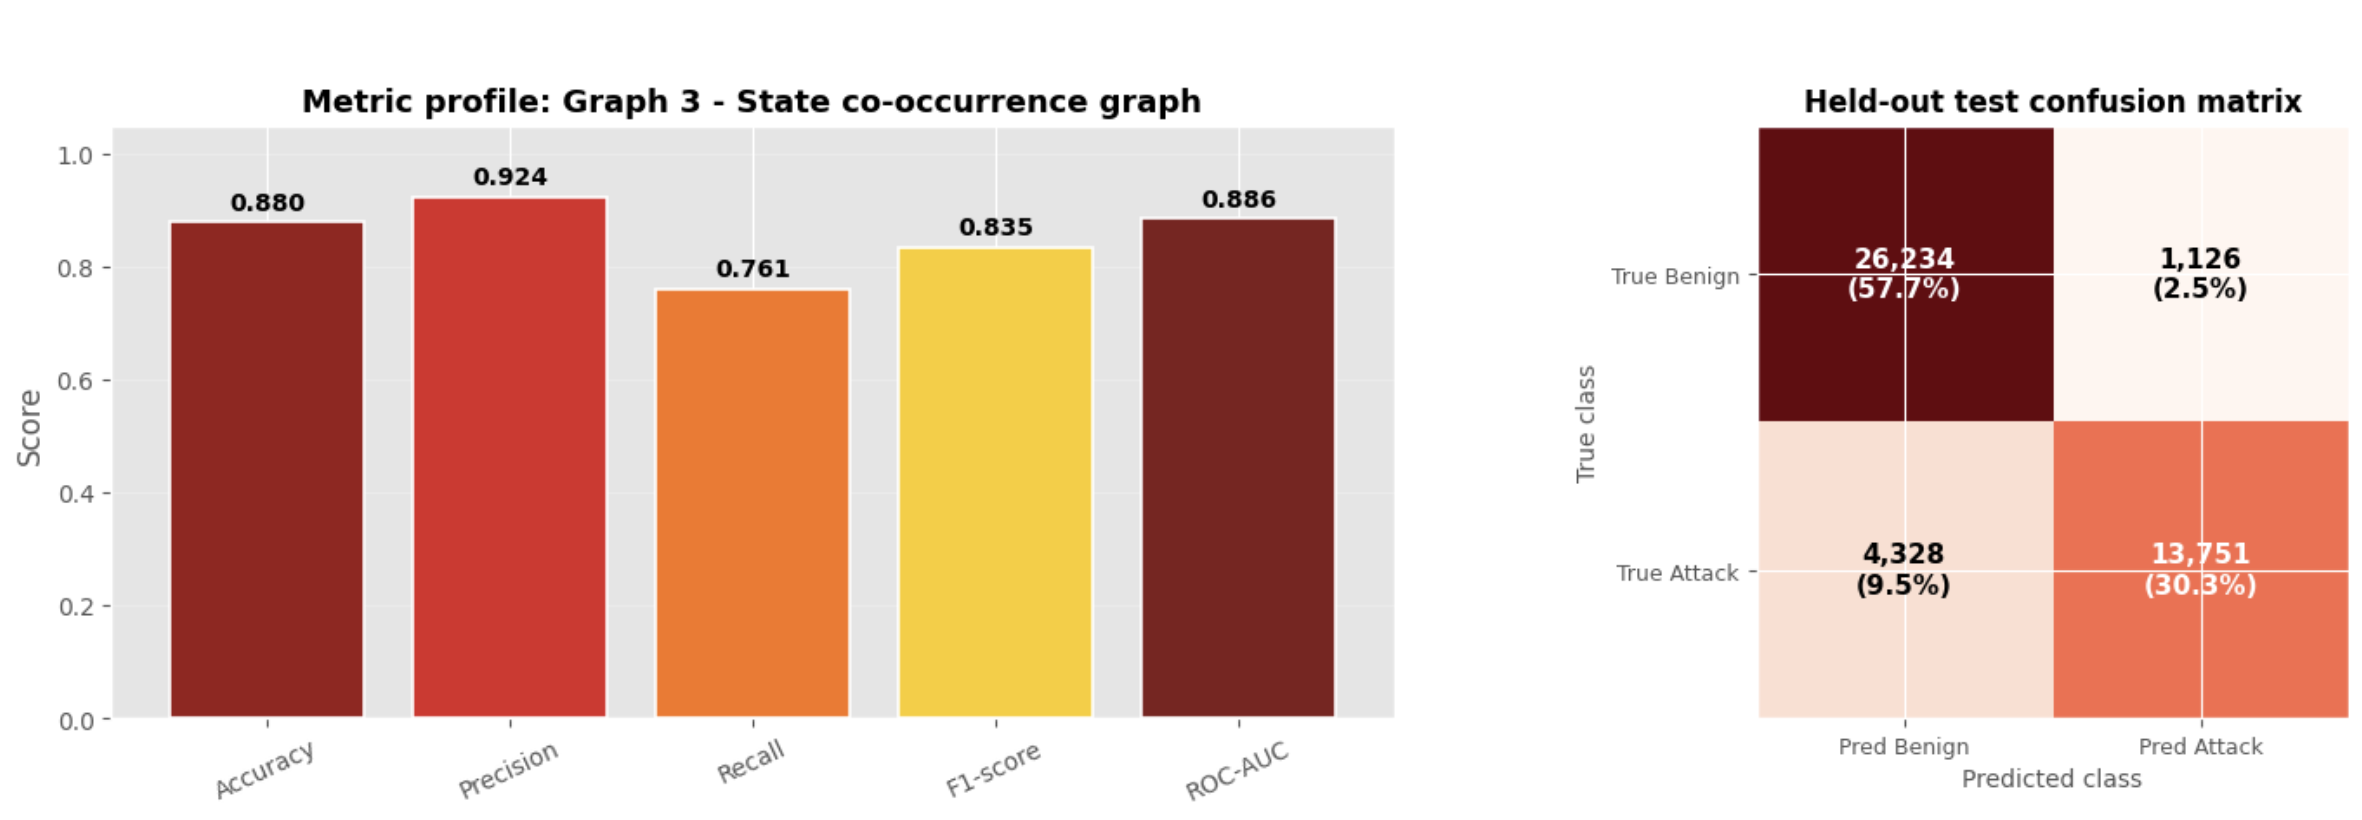
\includegraphics[width=\columnwidth]{figures/graph3.png}
    \caption{Held-out test performance of the state co-occurance graph, including evaluation metrics and confusion matrix}
    \label{fig:Graph 3 - Results and Confusion matrix Co-occurrence graph}
\end{figure}

\endgroup

\subsection{Graph Neural Networks (GNNs)}
\label{sec:Graph Neural Networks (GNNs)}
Neural Networks, often referred to as Deep Learning (DL), are an active area of research across many fields. They rose to prominence in the 1980s. DL includes Convolutional Neural Networks, which are used for image classification where have proven to be highly effective \citep{alma990016042380204808}.

Graph Neural Networks (GNNs) are also part of DL and have become a successful approach by learning useful representations from graph-structured data \cite{bilot2023graph}.  Cybersecurity practitioners have years of experience using graph analysis for capturing structural patterns in attack data. When we are able to represent the benign behavior of the IIoT devices as graphs. Attack behavior is characterized by a sequence of suspicious and normal behavior among entities, such as the host or processes within the host system. It is possible to capture this behavior and model it with a GNN to learn patterns in these interactions and achieve strong results applicable across various cybersecurity domains, such as threat intelligence, malware detection, and more \citep{bilot2023graph}.

\citet[p.~49118]{bilot2023graph} state that \textit{``GNN model can be applied to directed, undirected, labeled and cyclic graphs using the concept of neighbor information propagation.''}

A general Graph Neural Network (GNN) updates the representation of a node by combining its own features with information from its neighboring nodes. In this study, this idea is useful because an IIoT device or traffic-state node is not treated as isolated; instead, its representation can be influenced by the other nodes connected to it in the graph.

\[
h_u = f(x_u, x_v, h_v), \qquad u \in V,\; v \in \mathcal{N}(u)
\]

where \(h_u\) is the learned representation, or embedding, of node \(u\), \(x_u\) represents the input features of node \(u\), \(x_v\) represents the input features of a neighboring node \(v\), and \(h_v\) is the learned representation of that neighbor. The term \(\mathcal{N}(u)\) means the set of neighboring nodes connected to \(u\). In other words, the GNN learns the state of a node by aggregating information from its local graph neighborhood \citep{bilot2023graph}.

\begingroup
\color{red}
\subsubsection{Knowledge graph + Simple GNN}
\label{Knowledge graph + Simple GNN}
Now, we are going to use Graph Neural Networks, specifically Graph Convolutional Networks (GCNs), to see whether we obtain different results compared to the normal graph. For this initial KG+GNN, we will use the same simple structure we were using for the previous 3 normal graphs:

\begin{center}
\texttt{deviceName} \(\rightarrow\) \texttt{behaviorState}
\end{center}

GCNs are a deep learning approach used to represent Non-Euclidean data, such as social networks and graphs, and are an extension of CNNs \citep{jiang2019anomaly}.


Following the GCN formulation presented in the \cite{dgl_gcn_tutorial} documentation, a graph convolutional layer can be written as:

\[
H^{(l+1)}
=
\sigma
\left(
\tilde{D}^{-\frac{1}{2}}
\tilde{A}
\tilde{D}^{-\frac{1}{2}}
H^{(l)}
W^{(l)}
\right)
\]

where \(H^{(l)}\) is the node embedding matrix at layer \(l\), \(H^{(l+1)}\) is the updated node embedding matrix, \(W^{(l)}\) is the learnable weight matrix, and \(\sigma\) is a nonlinear activation function. The matrix \(\tilde{A} = A + I\) represents the adjacency matrix with self-loops, meaning that each node keeps part of its own information during message passing. The matrix \(\tilde{D}\) is the degree matrix of \(\tilde{A}\), and it is used to normalize the adjacency matrix so that nodes with many connections do not dominate the aggregation process.

This formula is equivalent to the compact GCN notation \citep{bilot2023graph}:

\[
H^{(l+1)}
=
\sigma
\left(
\hat{A}
H^{(l)}
W^{(l)}
\right)
\]

where the normalized adjacency matrix \(\hat{A}\) is defined as:

\[
\hat{A}
=
\tilde{D}^{-\frac{1}{2}}
\tilde{A}
\tilde{D}^{-\frac{1}{2}}
\]

Conceptually, the device representation can be written as:

\[
h_{\text{device}}
=
f(\text{deviceName}, \text{behaviorState})
\]

\begin{figure*}[t]
    \centering
    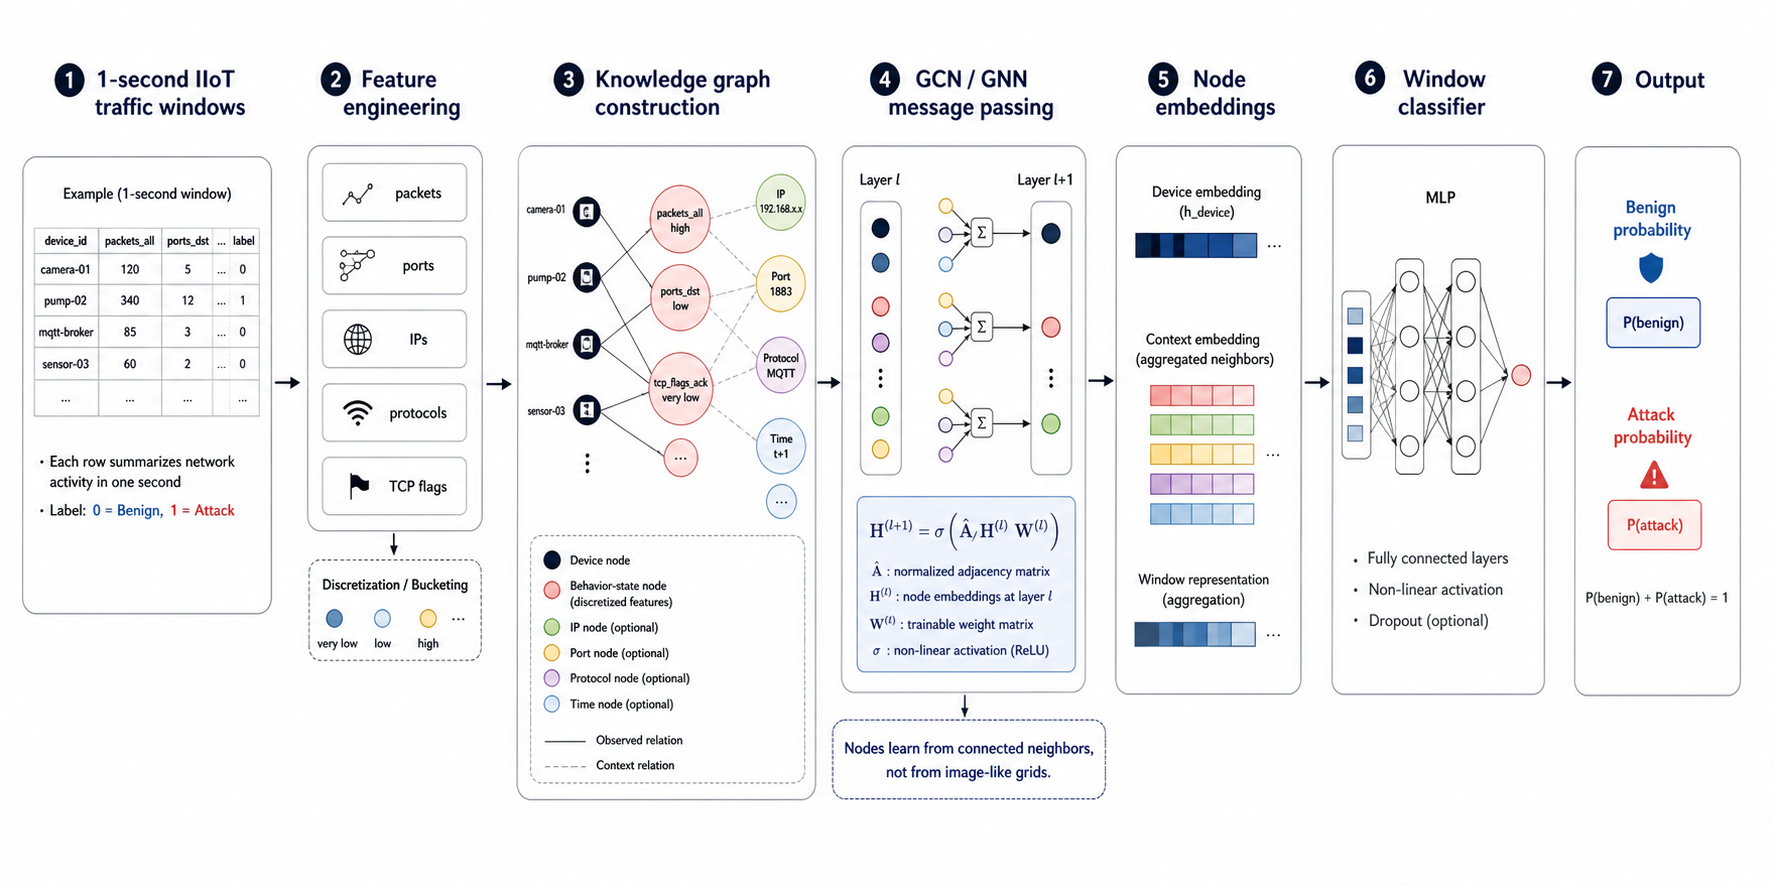
\includegraphics[width=0.85\textwidth]{figures/gnn_representation.png}
    \caption{Architecture of the GNN-based intrusion detection workflow, from 1-second IIoT traffic windows to knowledge graph construction, message passing, node embeddings, and benign-versus-attack classification -  generated by Codex 5.5 \citep{openai_gpt54_2026}.}
    
    \label{fig:gnn_representation}
\end{figure*}

We are going to train our Knowledge graph + Simple GNN with {20, 50, 80, 100, 150} epochs and analyze the best performance according to the validation F1-score The held-out test set is used only after selecting the best validation checkpoint. \cite{nebius2025epochs} gives us general recommendations on the amount of epochs to use in our simple GNN model according to the size of our dataset (227,191). The maximum epoch we used is 150, it does not mean we automatically decide to use 150 epochs for all the runs. Neural Networks can reach the best generalization earlier, hence, we train up to the maximum allowed epoch and keep the highest F1-score. Following this validation steps, it help to decide when the model generalizes best. To reduce randomness and improve reproducibility, experiments used fixed seeds (random\_state=42, np.random.seed(42), and torch.manual\_seed(42). However, because neural-network training can still exhibit nondeterministic behavior, especially with stochastic optimization and dropout, model selection was based on validation F1 rather than a fixed epoch number.

\begin{table}[H]
\caption{Hyperparameters used in the Simple GNN model.}
\centering
\small
\renewcommand{\arraystretch}{1.25}
\begin{tabular}{ll}
\hline
\textbf{Hyperparameter} & \textbf{Value} \\ \hline
\texttt{hidden\_dim} & \texttt{32} \\
\texttt{num\_layers} & \texttt{2} \\
\texttt{dropout} & \texttt{0.1} \\
\texttt{batch\_size} & \texttt{4096} \\
\texttt{learning\_rate} & \texttt{1e-3} \\
\texttt{optimizer} & \texttt{Adam} \\
\texttt{selection\_metric} & validation F1-score \\ \hline
\end{tabular}
\label{tab:simple_gnn_hyperparameters}
\end{table}

The \texttt{hidden\_dim} parameter defines the size of each node embedding, where each device or behavior-state node is represented by a vector of 32 learned values. The model uses two GCN message-passing layers, allowing nodes to learn from direct neighbors and indirect neighbors. A dropout value of \texttt{0.1} was used to reduce overfitting, while a batch size of \texttt{4096} defines the number of 1-second windows processed before updating the model weights. The learning rate was set to \texttt{1e-3}, equivalent to \texttt{0.001}, and the model was optimized using Adam. The best checkpoint was selected using the validation F1-score rather than the test set.



\begin{table}[H]
\centering
\caption{Simple GNN epoch sensitivity on the held-out test set.}
\label{tab:simple_gnn_epoch_sensitivity}
\resizebox{\columnwidth}{!}{%
\begin{tabular}{rrrrrrr}
\hline
Max Epochs & Best Epoch & Val. F1 & Acc. & Prec. & Rec. & F1 \\
\hline
20  & 19  & 0.79 & 0.85 & 0.91 & 0.71 & 0.79 \\
50  & 45  & 0.81 & 0.87 & 0.92 & 0.73 & 0.81 \\
80  & 80  & 0.82 & 0.87 & 0.92 & 0.75 & 0.82 \\
100 & 100 & 0.82 & 0.87 & 0.92 & 0.75 & 0.83 \\
150 & 106 & 0.83 & 0.88 & 0.92 & 0.76 & 0.83 \\
\hline
\end{tabular}
}
\end{table}


\begin{table}[H]
\centering
\caption{Simple GNN confusion-matrix counts by epoch setting.}
\label{tab:simple_gnn_confusion_by_epoch}
\resizebox{\columnwidth}{!}{%
\begin{tabular}{rrrrrr}
\hline
Max Epochs & Best Epoch & TN & FP & FN & TP \\
\hline
20  & 19  & 26021 & 1339 & 5277 & 12802 \\
50  & 45  & 26184 & 1176 & 4865 & 13214 \\
80  & 80  & 26115 & 1245 & 4513 & 13566 \\
100 & 100 & 26107 & 1253 & 4500 & 13579 \\
150 & 106 & 26143 & 1217 & 4286 & 13793 \\
\hline
\end{tabular}
}
\end{table}



\begin{figure}[H]
\centering
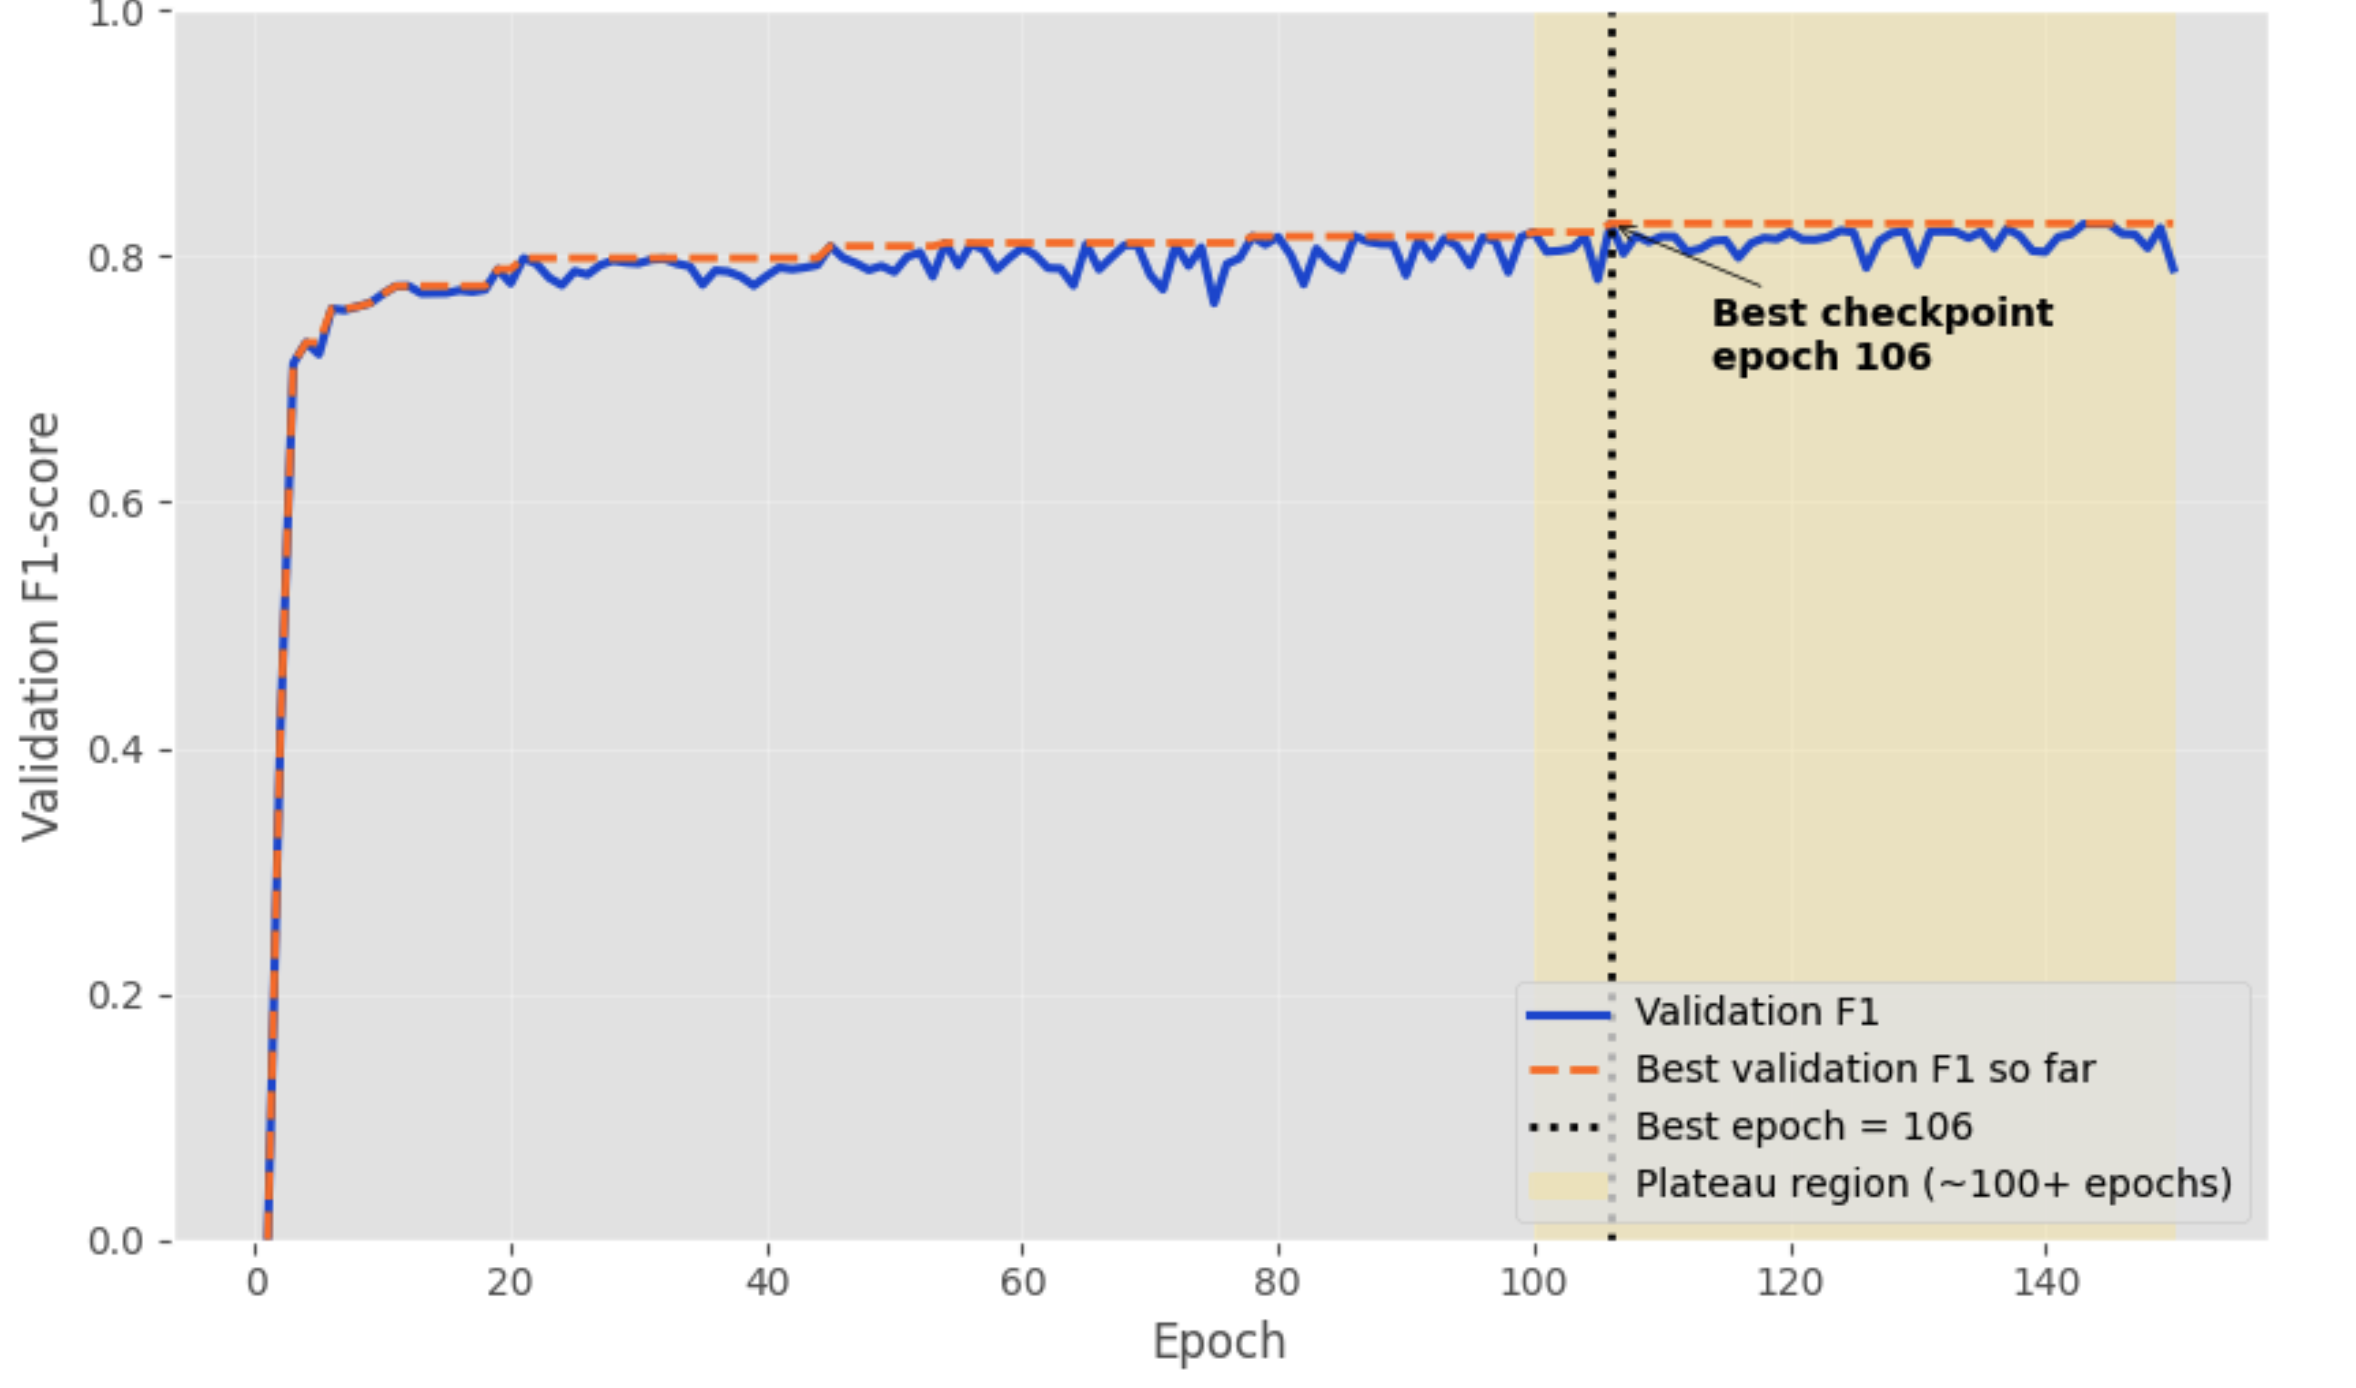
\includegraphics[width=\columnwidth]{figures/145epoch_simple_GNN.png}
\caption{Simple GNN validation F1 and learning plateau}
\label{fig:simple_gnn_learning_plateau}
\end{figure}


We ran several times our baseline model to get the best epoch performance and the results were close to a range between \texttt{100-150}. Hence, we see that the model reaches a performance plateau after approximately 100 epochs. The exact best checkpoint may vary across runs, but it generally occurs within the plateau region between 100 and 150 epochs. In a few words, every time we ran the model a with the same hyperparameters and same np.random.seeds(42) we were obtaining a different best epoch, for instance, \texttt{100, 106, 145}, therefore for this paper we chose best epoch 106, that makes sense as it is within the plateau region, see figure \ref{fig:simple_gnn_learning_plateau}.

\begin{figure}[H]
    \centering
    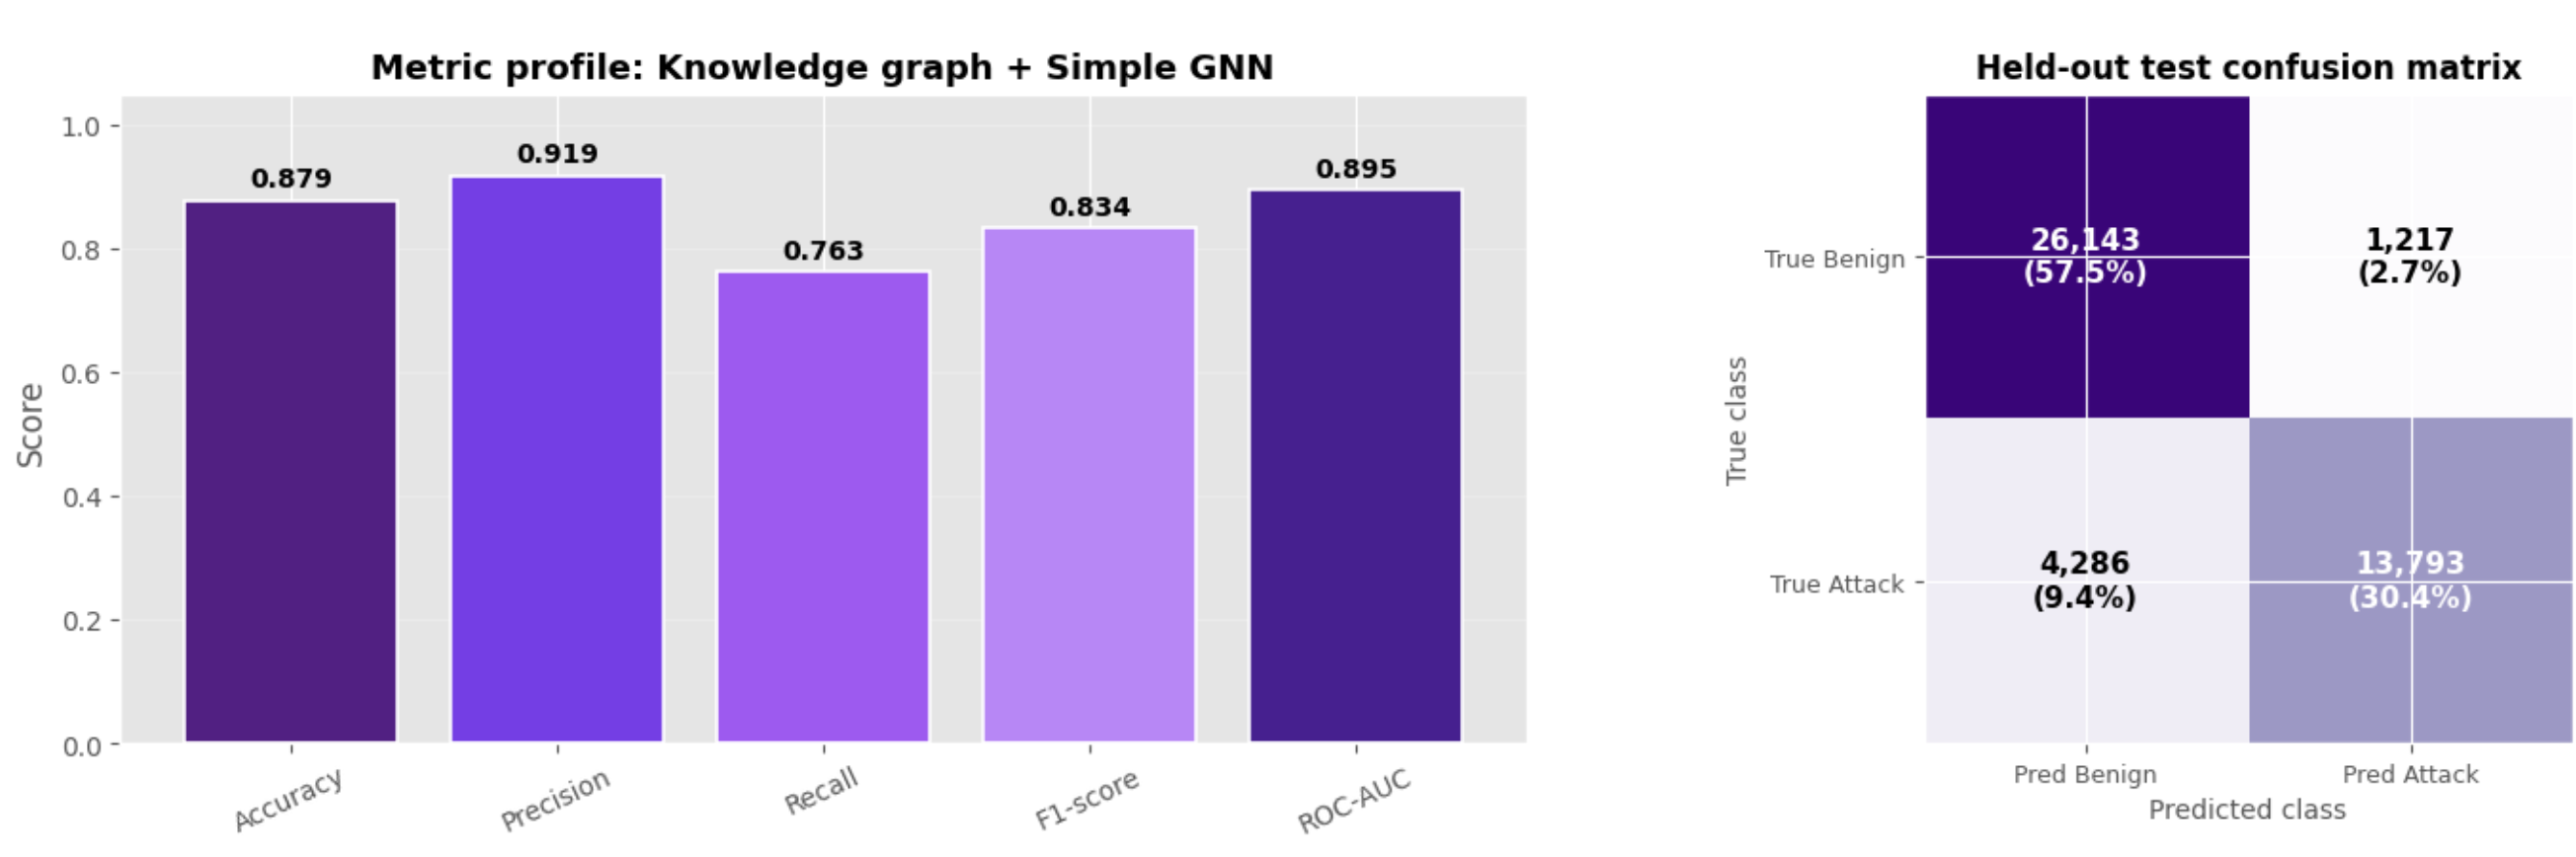
\includegraphics[width=\columnwidth]{figures/GNN-confusion matrix.png}
    \caption{Graph neural network confusion matrix}
    \label{fig:confusion matrix_GNN}
\end{figure}

Figure \ref{fig:gnn_representation} shows the step followed to obtain the overall performance results and confusion matrix of figure \ref{fig:confusion matrix_GNN}.
\endgroup

\subsubsection{Expansion of the Graph Structure}
\label{Expansion of the Graph Structure}
{\color{red}In the previous graph analysis, we tested a simple device-to-behavior-state. It was very useful, but comparing the results, it did not outperform the tabular methods, for instance, k-NN got a 0.92 accuracy, 0.97 in precision, and a recall of 0.83, and logistic regression got an accuracy of 0.90, precision of 0.95, and a recall of 0.79. The best graph method was the Dual Affinity-class graph in figure \ref{fig:graph2_affinity-class_results}, which achieved an accuracy of 0.8845, a precision of 0.92, and a recall of 0.78. Of all the methods tested in this study, the Dual Affinity-class ranked fifth. The idea was to test if graph-based methods can outperform classical tabular methods, but our results did not show that. Therefore, based on the literature of \citep{altaf_gnn-based_2024}, we decided to create a richer representation of the graph structure by expanding the initial device-to-behavior-state graph.}

\citep{altaf_gnn-based_2024} modeled IIoT graphs containing botnet traffic and created a heterogeneous multigraph representation of network topology, with the idea of capturing the temporal dynamics of network communication across devices.

\[
\begin{aligned}
G_{\text{rich}} &= (V_D, V_S, V_{IP}, V_P, V_R, V_T, E) \\
V_D &= \text{device nodes} \\
V_S &= \text{behavior-state nodes} \\
V_{IP} &= \text{IP nodes} \\
V_P &= \text{port nodes} \\
V_R &= \text{protocol nodes} \\
V_T &= \text{time nodes} \\
E &= E_{D,S} \cup E_{D,IP} \cup E_{D,P} \cup E_{D,R} \cup E_{D,T}
\end{aligned}
\]

where \(G_{\text{rich}}\) is the complete graph and \(E\) means the set of edges, or the connections within the graph.

{\color{red}The richer graph representation in this study expands the initial device-to-behavior-state graph by adding IP, port, protocol, and temporal nodes. \citep{bilot2023graph} also supports the idea that a simple structural representation of the graph like the one we did device-to-behavior-state fails to capture patterns that are pivotal for anomaly detection.} Cyber threats now come with new attack patterns that elapse arbitrary periods of time; consequently, \citep{bilot2023graph} advocate for a richer heterogeneous representation of graphs for better attack detection.

\begin{center}
\begin{tabular}{c}
\texttt{device} \(\rightarrow\) \texttt{behavior-state} \\
\texttt{device} \(\rightarrow\) \texttt{IP} \\
\texttt{device} \(\rightarrow\) \texttt{port} \\
\texttt{device} \(\rightarrow\) \texttt{protocol} \\
\texttt{device} \(\rightarrow\) \texttt{time} \\
\texttt{time} \(\rightarrow\) \texttt{next time}
\end{tabular}
\end{center}

This allows the graph to encode not only the device behavior state, but also where the communication occurs, which ports and protocols are involved, and when the traffic window appears.

Figure \ref{richer-heterogeneous-structure} is a representation of the richer graph structure created to capture patterns in the dataset.
{\color{red}To test one more time the GNNs using a richer heterogeneous graph structure in order to expand this study and answer our research question, we will compute the following three (3) GNN-richer models: GCN-rich, GraphSAGE-rich, and GAT-rich as explained in the work of \citep{bilot2023graph}. For this new evaluation the same hyperparameters shown in the Simple GNN device-behavior-state model in table \ref{tab:simple_gnn_hyperparameters} are used to make a fair comparison across the different GNN models.}

\begin{figure}[H]
    \centering
    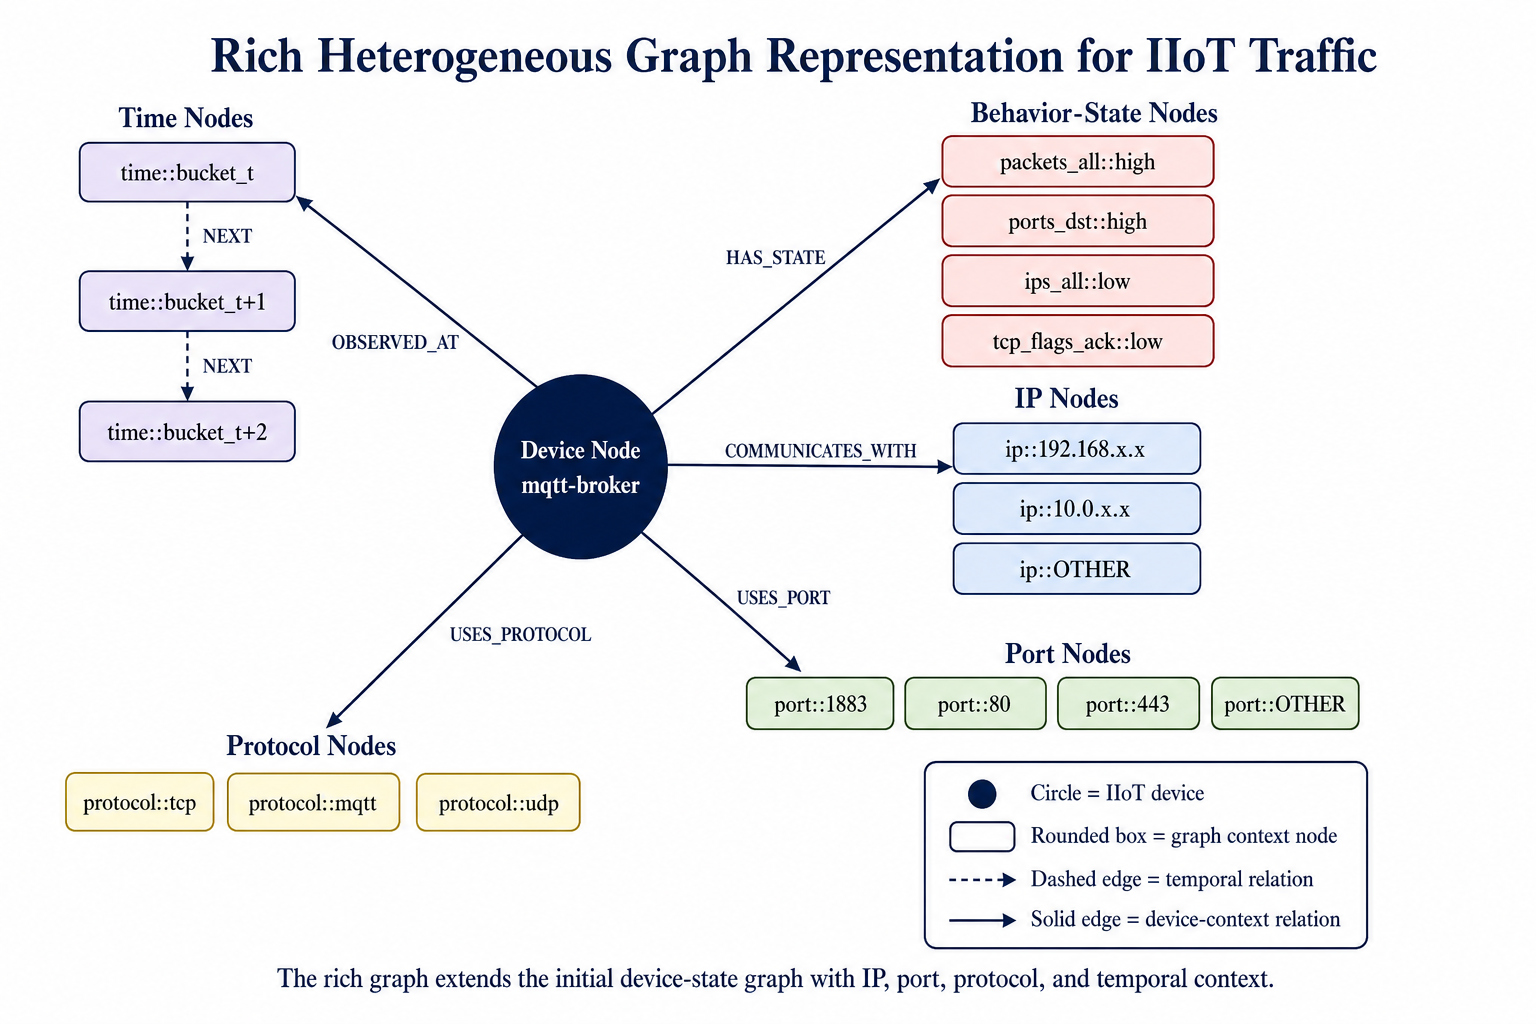
\includegraphics[width=\columnwidth]{figures/rich_heterogeneous_graph.png}
\caption{Rich heterogeneous graph structure connecting IIoT device nodes to behavioral states, IPs, ports, protocols, and temporal context -  generated by Codex 5.5 \citep{openai_gpt54_2026}.}
    \label{richer-heterogeneous-structure}
\end{figure}

%tabla-1
\begin{table}[H]
\caption{Node type summary for the rich graph representation.}
\centering
\small
\begin{tabular}{lr}
\toprule
\textbf{Node Type} & \textbf{Count} \\
\midrule
time & 7353 \\
port & 121 \\
ip & 82 \\
protocol & 41 \\
device & 38 \\
state & 33 \\
\bottomrule
\end{tabular}
\label{tab:node_type_summary}
\end{table}

%tabla-2
\begin{table}[H]
\caption{Edge type summary for the rich graph representation.}
\centering
\small
\begin{tabular}{lr}
\toprule
\textbf{Edge Type} & \textbf{Edge Count} \\
\midrule
device\_state & 1744812 \\
device\_ip & 302348 \\
device\_port & 245276 \\
device\_protocol & 196861 \\
device\_time & 145401 \\
time\_next & 7352 \\
\bottomrule
\end{tabular}
\label{tab:edge_type_summary}
\end{table}

\begin{center}
\textbf{Total nodes:} 7668\\
\textbf{Total unique typed edges:} 38093
\end{center}

Table~\ref{tab:node_type_summary} summarizes the node composition of the rich graph representation. Most nodes correspond to time nodes, followed by port, IP, protocol, device, and behavior-state nodes.

Table~\ref{tab:edge_type_summary} summarizes the edge types used to connect the different node categories in the rich graph. The largest number of observed relationships corresponds to device-state edges, followed by device-IP, device-port, device-protocol, and device-time relationships. The \texttt{time\_next} edges represent temporal continuity between consecutive time nodes.








\begingroup
\color{red}
\subsubsection{GCN-rich}
We use again a Graph Convolutional Neural Network (GCN), but this time with a richer graph structure. In our study, a device node learns of connected nodes such as behavior-state, IPs, ports, protocols and time nodes. It was chosen as baseline GNN because it is a classic and straightforward architecture for learning node embeddings using the graph structure.

The same formula used for simple GCN will be used for GCN-rich.

\[
H^{(l+1)}
=
\sigma
\left(
\tilde{D}^{-\frac{1}{2}}
\tilde{A}
\tilde{D}^{-\frac{1}{2}}
H^{(l)}
W^{(l)}
\right)
\]

The GCN-rich update rule remains the same as in the simple GCN. The difference is that the adjacency matrix \(A\) is now constructed from the richer graph structure, so the model propagates information across more types of nodes and relations.

In other words, the compact formula uses \(\hat{A}\) to represent the full normalized adjacency operation. In this study, \(A\) is built from the rich graph structure, including device-to-state, device-to-IP, device-to-port, device-to-protocol, device-to-time, and time bucket nodes.

After computing the results of the GCN-rich, we obtain the following result:

\begin{figure}[H]
    \centering
    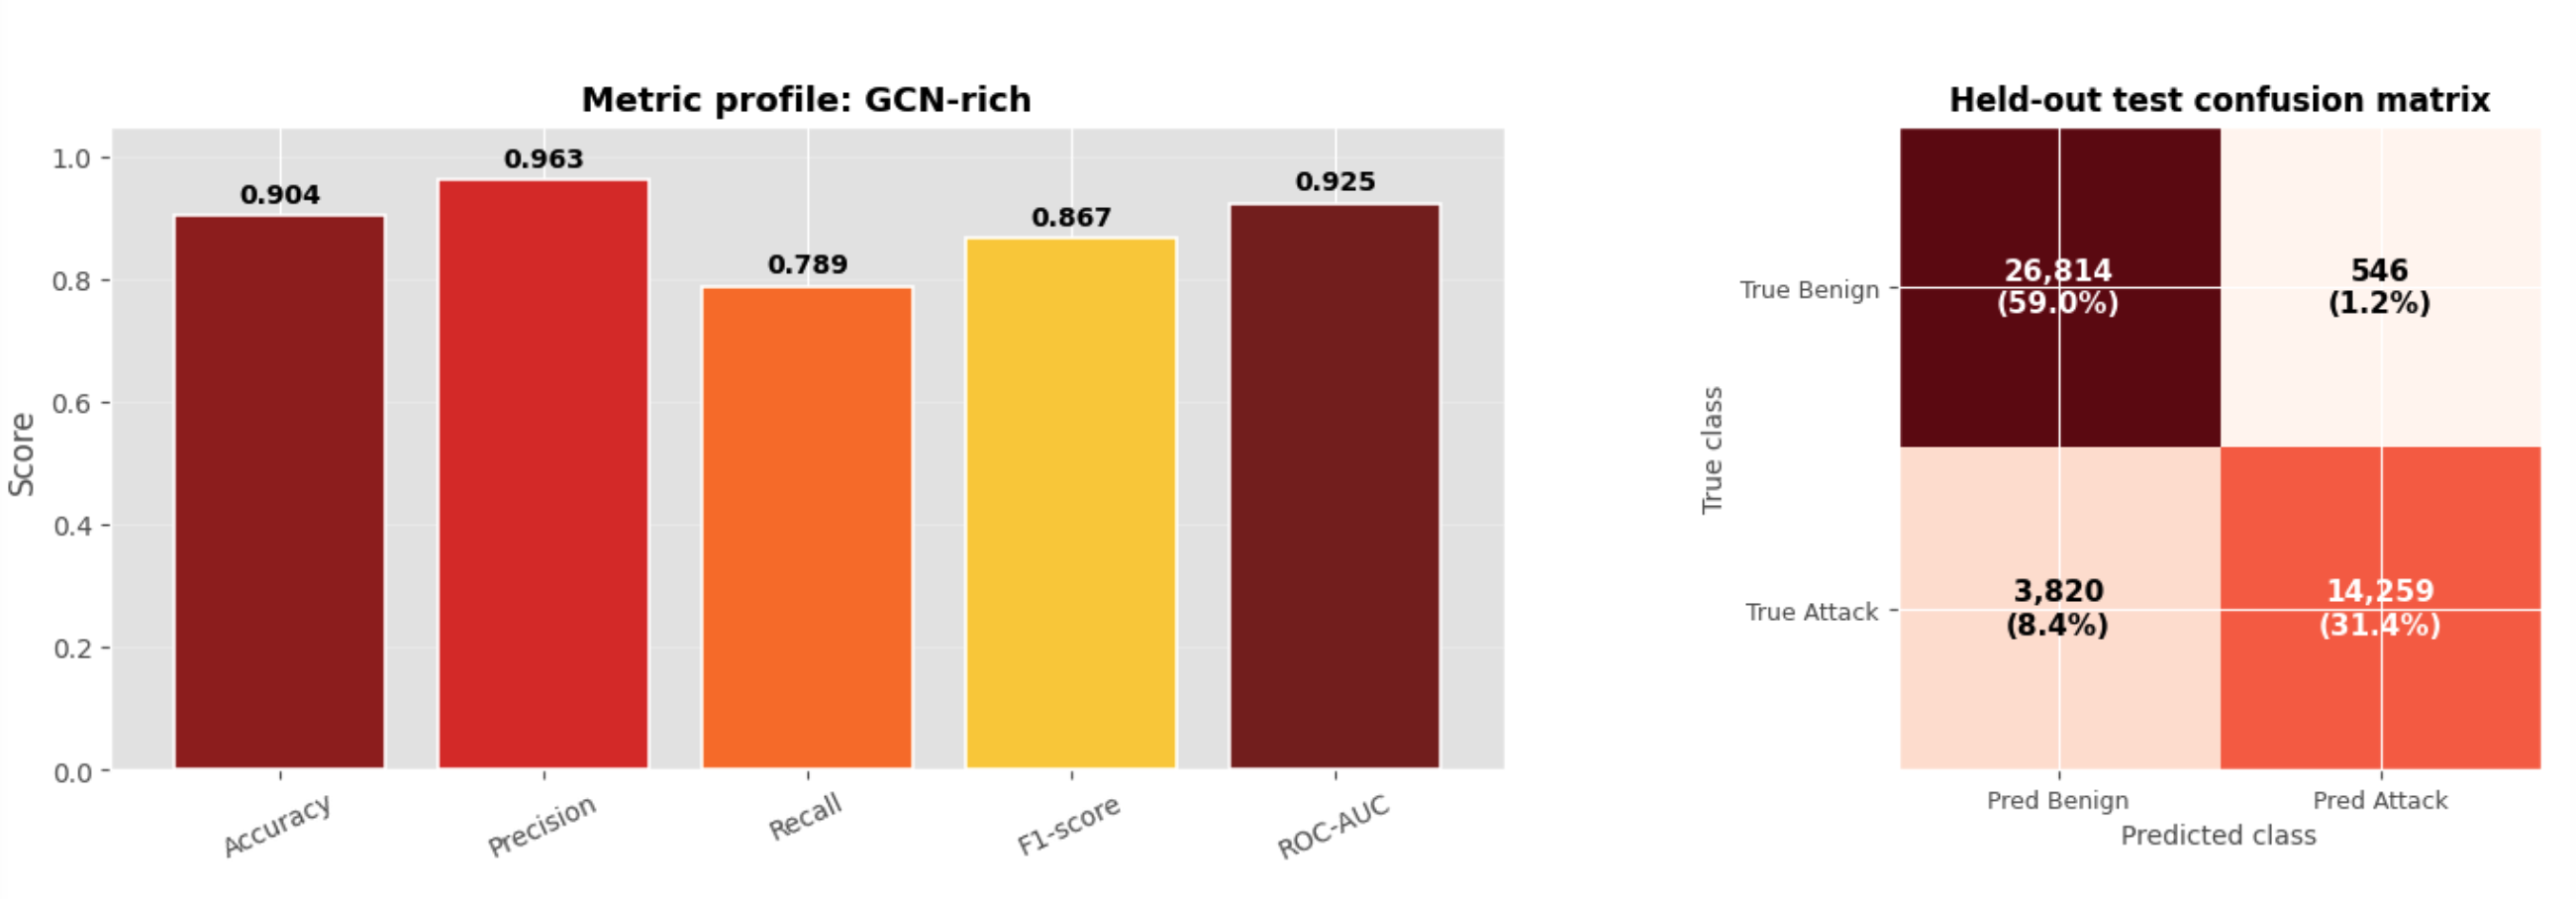
\includegraphics[width=\columnwidth]{figures/GCN-rich_results.png}
    \caption{Rich-graph GNN test profile: GCN-rich}
    \label{GCN-rich_results}
\end{figure}

\endgroup

\subsubsection{GraphSAGE-rich}
 GraphSAGE stands for Graph Sample and Aggregate. It is another method widely used in anomaly detection for IIoT devices. To use it for anomaly detection, when building the graph, the nodes are identified by an IP address and a port, the edges represent the communication between two nodes. It can be scaled up when new nodes added such as new devices, IPs or ports. GraphSAGE works mainly with node features and it used to learn embeddings of nodes \cite{bilot2023graph}. 


GraphSAGE was used as a second rich-graph GNN model because it is designed to learn node embeddings by sampling and aggregating information from a fixed number of neighboring nodes. Unlike a standard GCN, which uses the full adjacency matrix, GraphSAGE samples a subset of neighbors, making it more scalable for larger graphs. In this study, this is useful because the rich graph contains multiple node types, including devices, behavior states, IPs, ports, protocols, and time nodes.

Following the GraphSAGE formulation described by \citep{bilot2023graph}, the sampled neighborhood of node \(u\) is defined as:

\[
\mathcal{N}_s(u) = \mathrm{SAMPLE}(\mathcal{N}(u), s)
\]

where \(\mathcal{N}(u)\) is the full neighborhood of node \(u\), \(s\) is the number of sampled neighbors, and \(\mathcal{N}_s(u)\) is the sampled neighborhood.

The neighborhood aggregation step is defined as:

\[
h_{\mathcal{N}_s(u)}^{(l)}
=
\mathrm{AGGREGATE}^{(l)}
\left(
\left\{
h_v^{(l-1)}, \forall v \in \mathcal{N}_s(u)
\right\}
\right)
\]

where \(h_{\mathcal{N}_s(u)}^{(l)}\) is the aggregated representation of the sampled neighbors of node \(u\), and \(h_v^{(l-1)}\) is the embedding of neighbor node \(v\) from the previous layer.

The node update step is then defined as:

\[
h_u^{(l)}
=
\sigma
\left(
W^{(l)}
\cdot
\left[
h_u^{(l-1)}, h_{\mathcal{N}_s(u)}^{(l)}
\right]
\right)
\]

where \(h_u^{(l)}\) is the updated embedding of node \(u\), \(W^{(l)}\) is a learnable weight matrix, \(\sigma\) is a nonlinear activation function, and \([\cdot,\cdot]\) denotes concatenation. After running the GraphSAGE GNN model, we obtain the following results:

\begin{figure}[H]
\centering
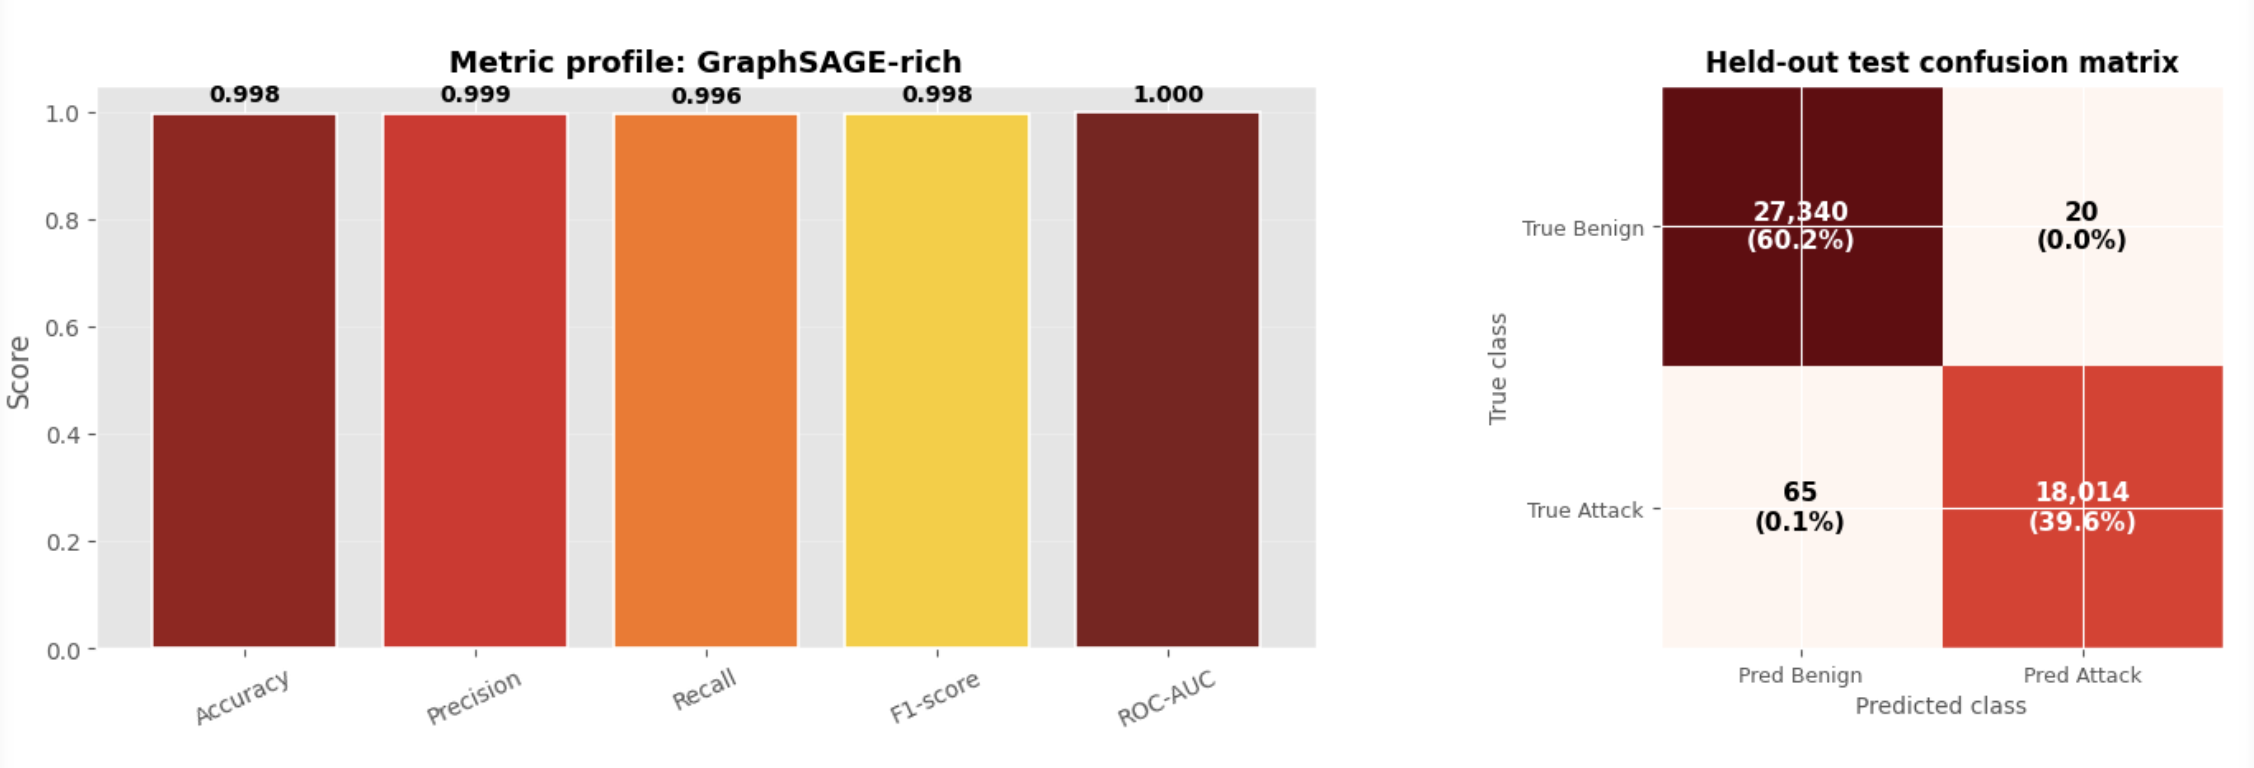
\includegraphics[width=\columnwidth]{figures/GraphSAGE-rich_results.png}
\caption{Rich-graph GNN test profile: GraphSAGE-rich}
\label{Rich-graph GNN test profile: GraphSAGE-rich}
\end{figure}






\subsubsection{GAT-rich}
GAT stands for Graph Attention Network. This GNN model can be used when the graph structure is evolving as it is very useful to generalize across diverse datasets and complex classification scenarios \citep{altaf_gnn-based_2024, ahmad2025gat}. However, \cite{bilot2023graph} say that can be unusable when working with large graphs billions of nodes or edges due to storage constraints. It stores in memory the whole adjacency matrix with corresponding features.

GAT uses an attention mechanism to assign a different importance scores to each neighbor of a node. Instead of aggregating all neighboring nodes with the same weight, GATs learn which neighbors are more relevant for the task. This allows the model to focus on more informative connections and produce a more refined aggregation of neighborhood information \citep{bilot2023graph}.

\[
\alpha_{uv}
=
\frac{
\exp\left(
\sigma\left(
a^{T}
[
Wh_u, Wh_v
]
\right)
\right)
}{
\sum_{k \in \mathcal{N}(u)}
\exp\left(
\sigma\left(
a^{T}
[
Wh_u, Wh_k
]
\right)
\right)
}
\]

the nodes update like:

\[
h'_u
=
\sigma
\left(
\sum_{v \in \mathcal{N}(u)}
\alpha_{uv}Wh_v
\right)
\]

In this formula, \(\alpha_{uv}\) is the attention coefficient between node \(u\) and its neighbor \(v\). The matrix \(W\) is a shared learnable weight matrix, \(a\) is a learnable attention vector, \(h_u\) and \(h_v\) are the node embeddings, and \(\mathcal{N}(u)\) is the neighborhood of node \(u\). The final embedding \(h'_u\) is computed as a weighted aggregation of the neighboring node embeddings, where more relevant neighbors receive higher attention weights \citep{bilot2023graph}.

We decided to use this model because in IIoT traffic, not all the connections are equally important. For instance, a specific port, IP or protocol may be more relevant than another when it comes to detecting attacks.

\begin{figure}[H]
\centering
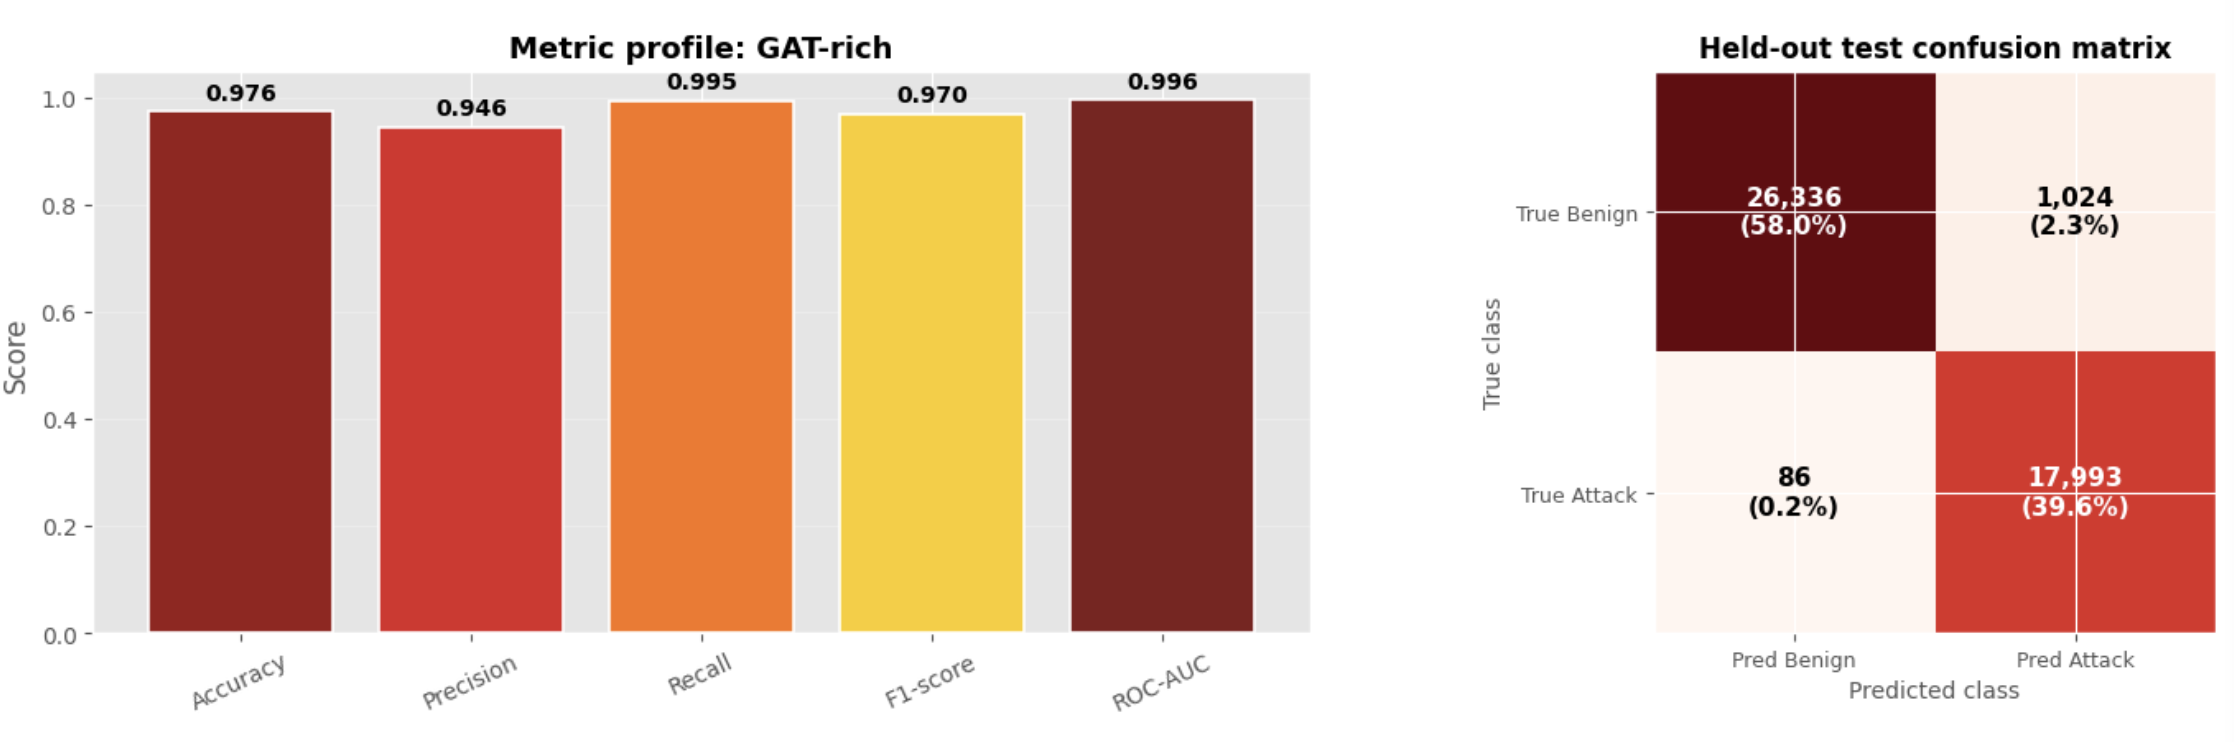
\includegraphics[width=\columnwidth]{figures/GAT-rich_results.png}
\caption{Rich-graph GNN test profile: GAT-rich}
\label{Rich-graph GNN test profile: GAT-rich}
\end{figure}


\section{Results}
\label{sec:results}
For the results section, we first compare the tabular models to identify which model performed best overall. {\color{red}Second, we analyze the graph-based models and the Simple GNN using the initial \texttt{device-behavior-state} structure.} Third, we evaluate the GNN models using the richer graph structure. Finally, we compare all models together and discuss their overall performance.

\subsection{Comparison of classical methods}
\label{comparisson of classical methods}

Our results show that the strongest performances in classical tabular methods are k-Nearest Neighbors (k-NN) with a precision of 0.98, recall of 0.84 and a F1-score of 0.90 and Logistic Regression with a precision of 0.96, recall of 0.78 and a F1-score of 0.86. k-NN as shown in previous studies is effective for generalization, showing high detection rates and low false positives \citep{alharthi2025comparative}. Other tabular methods such as LDA show strong classification overall based on the parameters. The worst was Naive Bayes for very little. These results show that classical tabular methods can still be useful for attack detection.

\begin{table}[H]
\caption{Train and test performance of tabular baseline models.}
\centering
\scriptsize
\setlength{\tabcolsep}{4pt}
\renewcommand{\arraystretch}{1.15}
\begin{tabular}{llcccc}
\toprule
\textbf{Model} & \textbf{Split} & \textbf{Precision} & \textbf{Recall} & \textbf{F1} & \textbf{ROC-AUC} \\
\midrule
Logistic Regression & Train & 0.96 & 0.78 & 0.86 & 0.91 \\
Logistic Regression & Test  & 0.95 & 0.79 & 0.86 & 0.91 \\
\midrule
Naive Bayes & Train & 0.95 & 0.75 & 0.83 & 0.88 \\
Naive Bayes & Test  & 0.94 & 0.75 & 0.84 & 0.88 \\
\midrule
LDA & Train & \textbf{0.99} & 0.73 & 0.84 & 0.90 \\
LDA & Test  & \textbf{0.98} & 0.74 & 0.84 & 0.90 \\
\midrule
QDA & Train & 0.97 & 0.75 & 0.84 & 0.90 \\
QDA & Test  & 0.97 & 0.75 & 0.85 & 0.90 \\
\midrule
k-NN & Train & 0.98 & \textbf{0.84} & \textbf{0.90} & \textbf{0.95} \\
k-NN & Test  & 0.97 & \textbf{0.83} & \textbf{0.90} & \textbf{0.93} \\
\bottomrule
\end{tabular}
\label{tab:tabular_train_test_booktabs}
\end{table}

\begin{figure}[H]
\centering
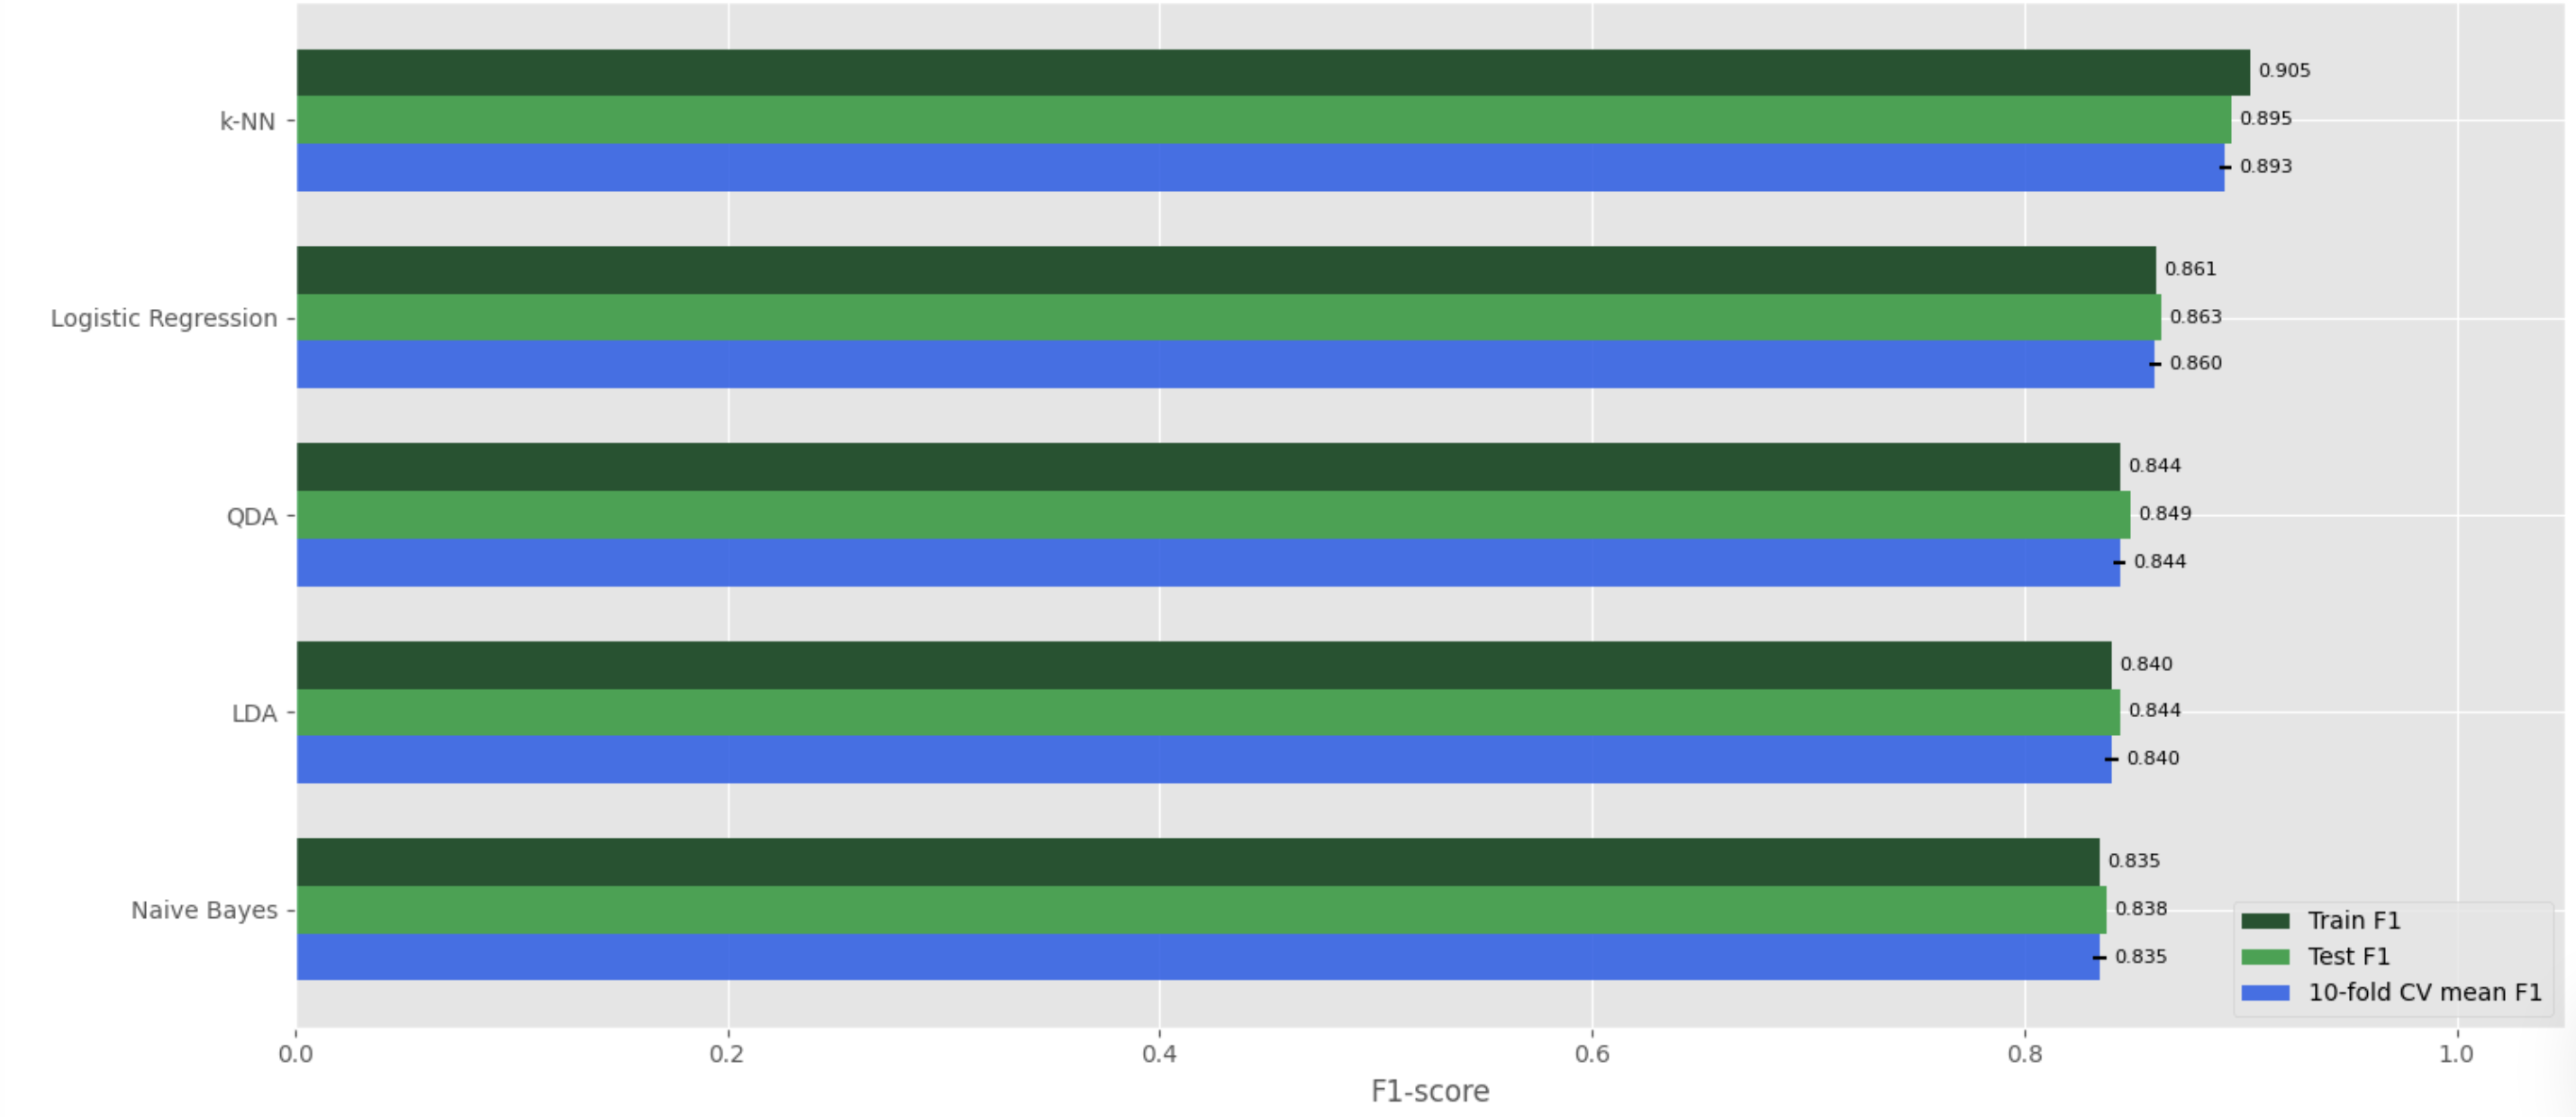
\includegraphics[width=\columnwidth]{figures/classical_methods_results_final.png}
\caption{Train vs test vs 10-fold CV F1-score by model}
\label{Train vs test vs 10-fold CV F1-score by model}
\end{figure}


\begingroup
\color{red}
\subsection{Graphs analysis}
\label{graph analysis}
We cannot discard the graph entirely; the graph analysis methods and the Knowledge Graph + GNN prototype captured meaningful signals, but overall, they did not surpass the best tabular model on the held-out test set. Among the graph-based approaches, Graph 2 (Dual-Class Affinity Graph) produced the strongest result, as shown in Table~\ref{tab:graph_analysis_gnn_performance_vertical}, indicating that comparing attack support against benign support is more effective than relying solely on simple state co-occurrence.

\begin{table}[H]
\caption{Performance comparison of graph-analysis methods and Simple GNN.}
\centering
\scriptsize
\renewcommand{\arraystretch}{1.15}
\begin{tabular}{llc}
\toprule
\textbf{Model} & \textbf{Metric} & \textbf{Value} \\
\midrule

\multirow{5}{*}{Graph 2 -- Dual-class affinity graph}
& Accuracy & \textbf{0.88} \\
& Precision & 0.92 \\
& Recall & \textbf{0.78} \\
& F1 & \textbf{0.84} \\
& ROC-AUC & \textbf{0.90} \\
\midrule

\multirow{5}{*}{Graph 3 -- State co-occurrence graph}
& Accuracy & 0.88 \\
& Precision & 0.92 \\
& Recall & 0.76 \\
& F1 & 0.83 \\
& ROC-AUC & 0.89 \\
\midrule

\multirow{5}{*}{Knowledge graph + Simple GNN}
& Accuracy & 0.88 \\
& Precision & 0.92 \\
& Recall & 0.76 \\
& F1 & 0.83 \\
& ROC-AUC & 0.90 \\
\midrule

\multirow{5}{*}{Graph 1 -- Benign novelty graph}
& Accuracy & 0.82 \\
& Precision & \textbf{1.00} \\
& Recall & 0.55 \\
& F1 & 0.71 \\
& ROC-AUC & 0.78 \\
\bottomrule

\end{tabular}
\label{tab:graph_analysis_gnn_performance_vertical}
\end{table}

We can see that Benign novelty graph reached a strong result of 1.00 precision. This means that when the model predicts attack, it is almost always right, however, the low recall of 0.55 also means that tends to miss most attacks. The best method taking into account the overall result is Dual-class affinity graph with an accuracy of 0.88, precision of 0.92 and a F1-score of 0.84. Simple structure device-behavior-state GCN did not make a good improvement overall.
\endgroup

\subsection{Exploring richer GNNs}
\label{Exploring richer GNNs}
After the graph expansion to a richer graph structure, our model obtained more attack detecting power as shown in table \ref{tab:rich_gnn_performance_vertical}. The best GNN was GraphSAGE-rich that reached an almost perfect overall result (accuracy = 0.9979, precision = 0.9976, recall = 0.9970, F1 = 0.9973). The second model GNN model with the best performance was GAT-rich (accuracy = 0.9629, precision = 0.9562, recall = 0.9502, F1 = 0.9532). {\color{red}We cannot discard GCN-rich (accuracy = 0.9054, precision = 0.8787, recall = 0.8842, F1 = 0.8815), which also showed high efficiency for attack detection.}


\begin{table}[H]
\caption{Rich-graph GNN model comparison.}
\centering
\scriptsize
\renewcommand{\arraystretch}{1.15}
\begin{tabular}{llr}
\toprule
\textbf{Model} & \textbf{Metric} & \textbf{Value} \\
\midrule

\multirow{6}{*}{GraphSAGE-rich}
& Best epoch & 100 \\
& Accuracy & \textbf{0.9979} \\
& Precision & \textbf{0.9976} \\
& Recall & \textbf{0.9970} \\
& F1-score & \textbf{0.9973} \\
& ROC-AUC & \textbf{0.9998} \\
\midrule

\multirow{6}{*}{GAT-rich}
& Best epoch & 100 \\
& Accuracy & 0.9629 \\
& Precision & 0.9562 \\
& Recall & 0.9502 \\
& F1-score & 0.9532 \\
& ROC-AUC & 0.9879 \\
\midrule

\color{red}\multirow{6}{*}{GCN-rich}
& \color{red}Best epoch & \color{red}150 \\
& \color{red}Accuracy & \color{red}0.9054 \\
& \color{red}Precision & \color{red}0.8787 \\
& \color{red}Recall & \color{red}0.8842 \\
& \color{red}F1-score & \color{red}0.8815 \\
& \color{red}ROC-AUC & \color{red}0.9374 \\
\bottomrule
\end{tabular}
\label{tab:rich_gnn_performance_vertical}
\end{table}


The confusion matrix table below, we can observe that GraphSAGE-rich and GAT-rich are the best GNN models. For instance, GraphSAGE-rich is strong for detecting attacks (18,025) in IIoT devices and misses a few attacks (54).

\begin{table}[H]
\caption{Rich-graph GNN confusion-matrix counts.}
\centering
\small
\setlength{\tabcolsep}{5pt}
\renewcommand{\arraystretch}{1.20}
\begin{tabular}{lrrrr}
\toprule
\textbf{Model} & \textbf{TN} & \textbf{FP} & \textbf{FN} & \textbf{TP} \\
\midrule
GraphSAGE-rich & 27,317 & 43 & 54 & 18,025 \\
GAT-rich       & 26,574 & 786 & 901 & 17,178 \\
\color{red}GCN-rich & \color{red}25,154 & \color{red}2,206 & \color{red}2,093 & \color{red}15,986 \\
\bottomrule
\end{tabular}
\label{tab:rich_gnn_confusion_counts}
\end{table}

 After several runs, the best epochs were something in between 80 and 140 as shown on the plateau region in figure \ref{Validation F1 learning plateau by rich-graph GNN model}.


    \begin{figure}[H]
\centering
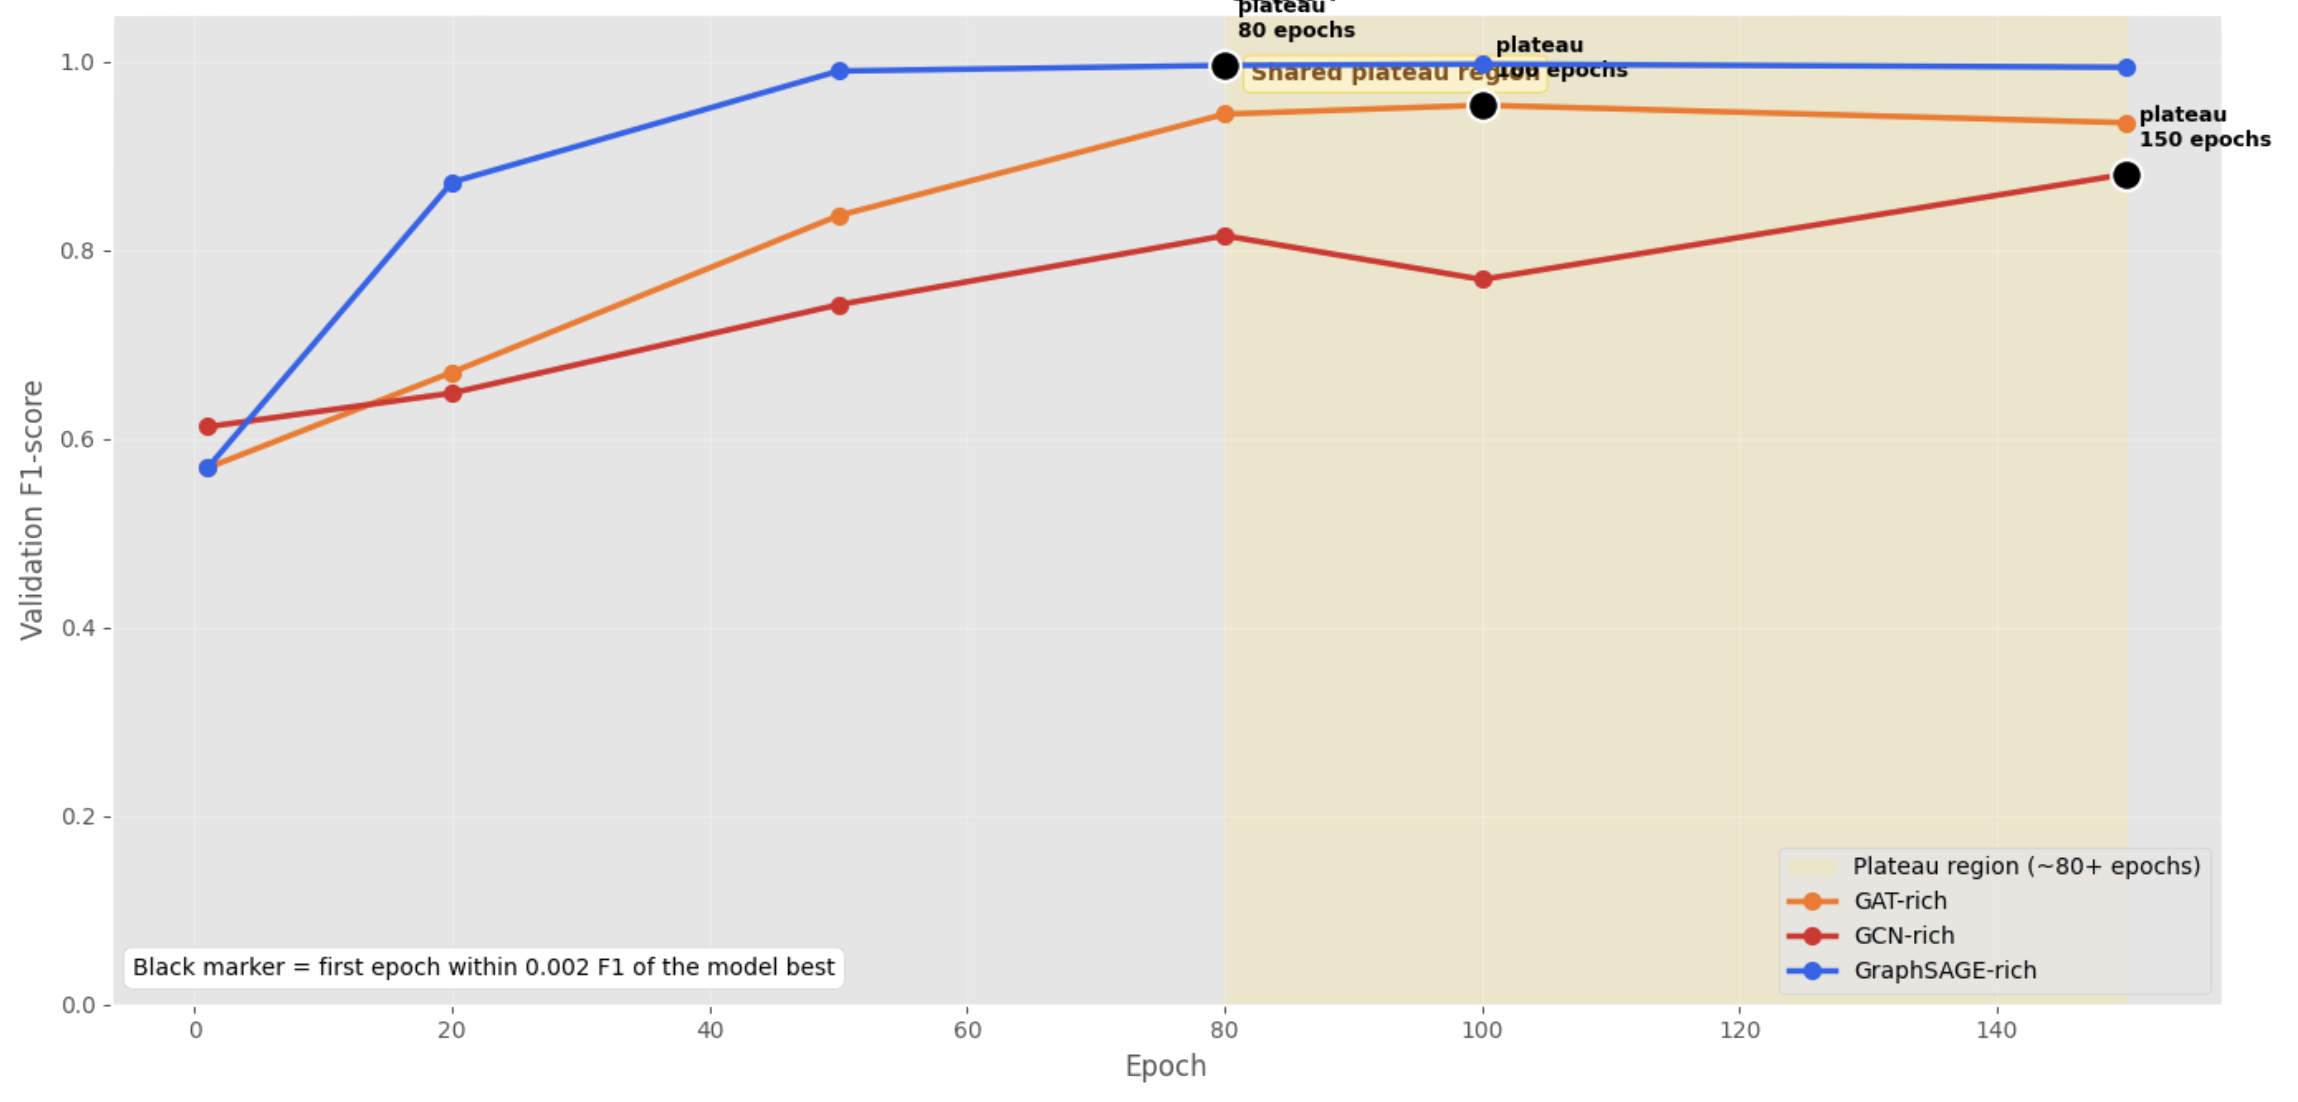
\includegraphics[width=\columnwidth]{figures/Validation F1 learning plateau by rich-graph GNN model.png}
\caption{Validation F1 learning plateau by rich-graph GNN model}
\label{Validation F1 learning plateau by rich-graph GNN model}
\end{figure}



\clearpage
\onecolumn

\subsection{Compare against previous methods}
\label{compare_against_previous_methods}

Our research question was if GNN can have a good performance over tabular classical methods? Under the current random window-level split, rich-graph GNNs outperformed the tabular baselines.

\begin{table}[H]
\caption{Overall model performance comparison.}
\centering
\footnotesize
\setlength{\tabcolsep}{4.5pt}
\renewcommand{\arraystretch}{1.12}
\begin{tabular}{lcccccccccc}
\toprule
\textbf{Model} & \textbf{Acc.} & \textbf{Prec.} & \textbf{Rec.} & \textbf{F1} & \textbf{ROC-AUC} & \textbf{TN} & \textbf{FP} & \textbf{FN} & \textbf{TP} & \textbf{MAR} \\
\midrule
GraphSAGE-rich & \textbf{0.9979} & 0.9976 & \textbf{0.9970} & \textbf{0.9973} & \textbf{0.9998} & 27317 & 43 & 54 & 18025 & \textbf{0.0030} \\
GAT-rich & 0.9629 & 0.9562 & 0.9502 & 0.9532 & 0.9879 & 26574 & 786 & 901 & 17178 & 0.0498 \\
k-NN & 0.9229 & 0.9723 & 0.8299 & 0.8954 & 0.9310 & 26933 & 427 & 3075 & 15004 & 0.1701 \\
\color{red}GCN-rich & \color{red}0.9054 & \color{red}0.8787 & \color{red}0.8842 & \color{red}0.8815 & \color{red}0.9374 & \color{red}25154 & \color{red}2206 & \color{red}2093 & \color{red}15986 & \color{red}0.1158 \\
Logistic Regression & 0.9005 & 0.9541 & 0.7878 & 0.8630 & 0.9129 & 26675 & 685 & 3836 & 14243 & 0.2122 \\
QDA & 0.8934 & 0.9709 & 0.7547 & 0.8492 & 0.9037 & 26951 & 409 & 4435 & 13644 & 0.2453 \\
LDA & 0.8915 & 0.9834 & 0.7399 & 0.8445 & 0.9018 & 27134 & 226 & 4702 & 13377 & 0.2601 \\
\color{red}Graph 2 & \color{red}0.8845 & \color{red}0.9210 & \color{red}0.7762 & \color{red}0.8424 & \color{red}0.9018 & \color{red}26156 & \color{red}1204 & \color{red}4046 & \color{red}14033 & \color{red}0.2238 \\
Naive Bayes & 0.8841 & 0.9449 & 0.7525 & 0.8378 & 0.8826 & 26567 & 793 & 4475 & 13604 & 0.2475 \\
\color{red}Graph 3 & \color{red}0.8800 & \color{red}0.9243 & \color{red}0.7606 & \color{red}0.8345 & \color{red}0.8857 & \color{red}26234 & \color{red}1126 & \color{red}4328 & \color{red}13751 & \color{red}0.2394 \\
\color{red}Simple GNN & \color{red}0.8789 & \color{red}0.9189 & \color{red}0.7629 & \color{red}0.8337 & \color{red}0.8952 & \color{red}26143 & \color{red}1217 & \color{red}4286 & \color{red}13793 & \color{red}0.2371 \\
\color{red}Graph 1 & \color{red}0.8214 & \color{red}\textbf{0.9995} & \color{red}0.5514 & \color{red}0.7107 & \color{red}0.7756 & \color{red}27355 & \color{red}5 & \color{red}8110 & \color{red}9969 & \color{red}0.4486 \\
\bottomrule
\end{tabular}

\vspace{0.05cm}
\noindent\textit{Note.} MAR = missed attack rate.

\label{tab:overall_model_performance_updated}
\end{table}

\begin{figure}[H]
    \centering
    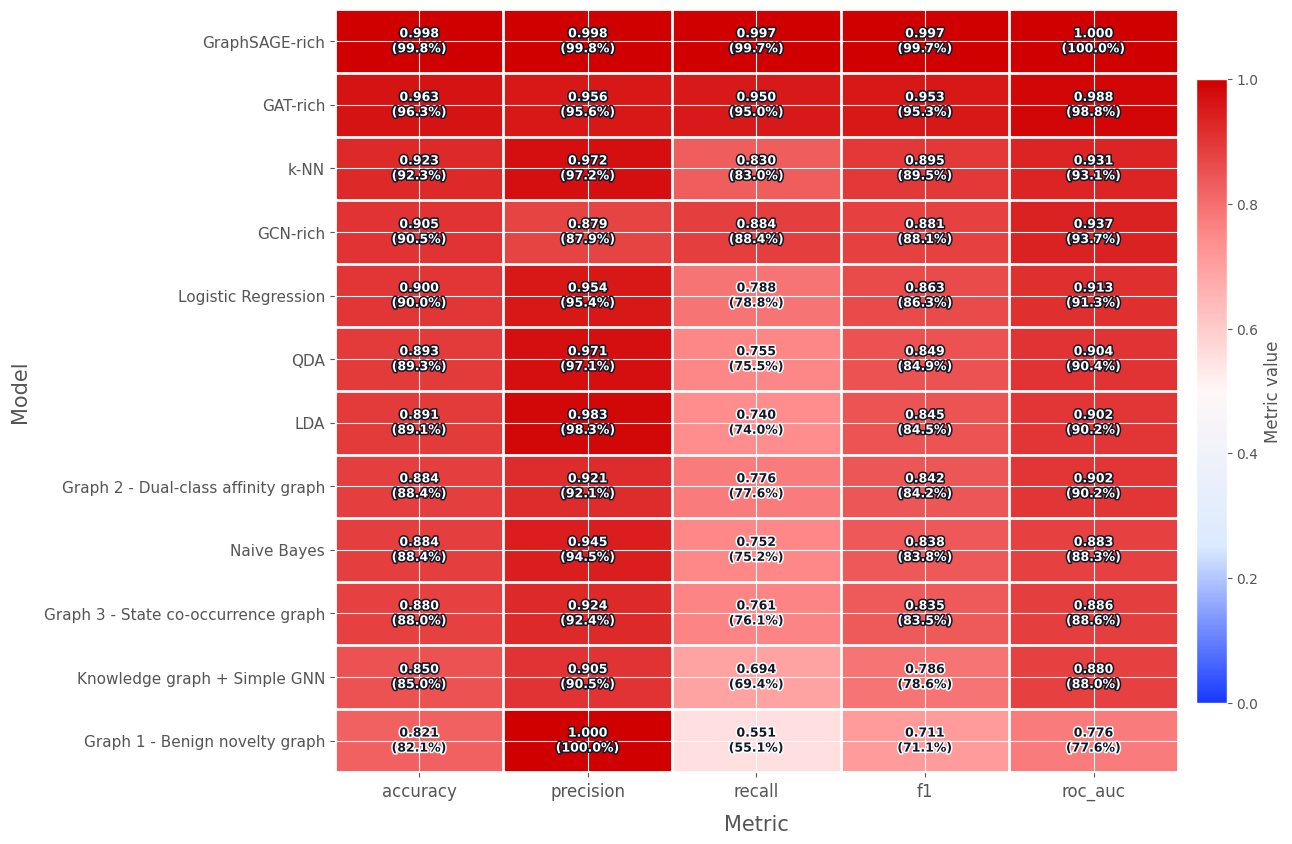
\includegraphics[width=0.92\textwidth]{figures/final_heatmap_all_models.png}
    \caption{{\color{red}REMOVE OR REPLACE FOR VERSION 2: this heatmap includes Graphs 1--3, the Simple GNN, and GCN-rich.} Final heatmap comparing all models across classification metrics.}
    \label{fig:final_heatmap_all_models}
\end{figure}

Table~\ref{tab:overall_model_performance_updated} compares all models using classification metrics, confusion-matrix counts, and the missed attack rate. Figure~\ref{fig:final_heatmap_all_models} provides a visual comparison of all models across accuracy, precision, recall, F1-score, and ROC-AUC. The heatmap confirms that GraphSAGE-rich achieves the strongest overall performance, with near-perfect values across all metrics. GAT-rich is the second strongest model and also outperforms the classical baselines in most metrics. Among the classical models, k-NN remains the best-performing non-graph approach. {\color{red}The graph heuristics and the Simple KG+GNN capture useful signal, but they remain below the rich graph GNN models. Graph 1 shows the highest precision, but its low recall indicates that it misses many attack windows.} Overall, the heatmap supports the conclusion that the richer graph representation improves intrusion detection performance when combined with stronger GNN architectures. 

\clearpage
\twocolumn

\section{Discussion and future work}
\label{Discussion}
For future work in this field, one could explore combining complementary detection behaviors from multiple approaches rather than selecting a single best model. A high-recall configuration can be used to minimize missed attacks, a high-precision configuration to reduce false positives, and low-confidence cases can be routed to an intermediate reviewer category for human inspection. Adjusting thresholds can trade off missed attacks against false positives.

Another recommendation is to evaluate graph models separately by attack family and by device type, rather than only using a single combined binary classifier. This would make it possible to determine whether graph-based learning performs consistently across devices and attack categories, or whether its performance is driven by specific device-attack patterns.

Although this study compares several classical baselines with graph-based approaches, other machine learning methods, such as Random Forest and XGBoost, were outside the scope of this analysis. These methods will be considered in future research, either as an expansion of the present work or in experiments using another dataset. {\color{red}One example could be creating a 3rd class adjusting the threshold on the graphs, in figure \ref{fig:State co-occurence score distribution on the test set} the resulting threshold was -0.082 but could in an expansion of this research create a review zone to review the uncertain for better generalization:}
{\color{red}
\[
\begin{cases}
\text{score} < -0.082 & \rightarrow \text{benign} \\
-0.082 \leq \text{score} \leq 0.082 & \rightarrow \text{uncertain} \\
\text{score} > 0.082 & \rightarrow \text{attack}
\end{cases}
\]
}

Further analysis is recommended on a similar dataset with nearly equal proportions of benign and attack data to train the models. A more balance dataset could improve performance of classical tabular methods.

We could also test graph models separately by device and attack type to verify whether performance generalizes across IIoT scenarios.


\begin{itemize}
    \item by attack type
    \item by device
    \item by device-attack combination
\end{itemize}

For instance, an attack performed on a mqtt-broker device can contain different patterns of ports and protocols than an attack on a camera or a sensor.

This study focuses on predictive performance and graph representation design. Concepts such as entropy-based traffic characterization, notebook latency, and neural-network execution time were outside the scope of the current analysis. These aspects may be considered in future work, especially for evaluating computational efficiency and real-time deployment feasibility.

Another method that could also been taken in consideration is Ridge and Lasso. These methods apply penalties on the feature that do not value to the model,  for a more efficient feature selection.\citep{alma990016042380204808}. 
Another technique is wrapper method that evaluates subsets of features based on model performance for datasets with large volumes of data \citep{ahmed2025pcm}.

\section{Limitations}
\label{Limitations}

\subsection{Proportion of the dataset}
The benign and attack classes are not perfectly balanced in our combined dataset (Benign: 136,800 observations; Attack has 90,391 observations; approximately 60/40). While it can considered this a moderate imbalance overall, it can be worse at the device level and may bias models toward the majority patterns, for example, detecting more benign behavior than attack, affecting precision,  sensitivity, ROC-AUC, and threshold selection. We therefore used stratified splits and k-fold cross-validation to mitigate this issue. \cite{akoglu2015graph} says that unbalanced data is a big challenged since anomalies in the data are very rare and represent a smaller fraction of the whole observation.
\begin{figure}[H]
    \centering
    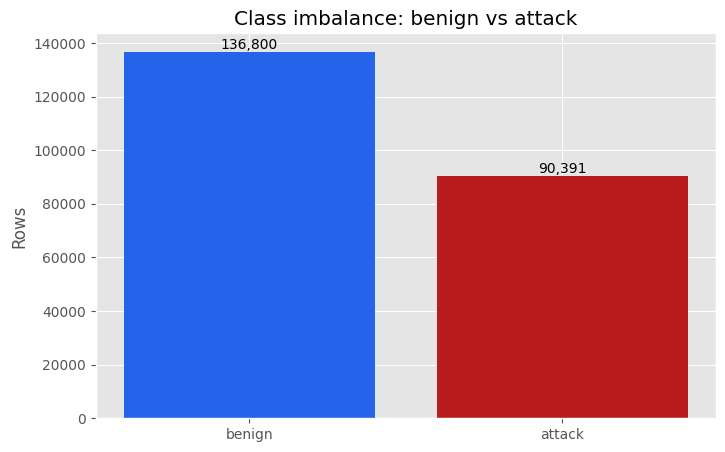
\includegraphics[width=\columnwidth]{figures/class_imbalance.png}
    \caption{Class imbalance.}
    \label{fig:class_imbalance}
\end{figure}
\subsection{Computational constraints}
Computing power available to make my work more efficient was critical limitation.


\section{Conclusion}
\label{Conclusion} 
In this study, we evaluated whether graph-based intrusion detection analysis using a knowledge graph and a graph neural network (GNN) can outperform tabular models for IIoT attack detection on CIC IIoT 2025 1-second windows.

Our analysis showed that benign traffic is typically sparse and can become bursty, depending on the traffic observed on the device. Attack traffic exhibits much higher packet activity, is more bursty, and shows distinct structural patterns in the plots presented.

Graph Neural Networks exhibited the strongest performance for attack detection after enriching the graph structure, as they captured more attacks than the highest-performing tabular method, k-NN. Classical tabular methods remain relevant because they are easier to interpret and less time-consuming to compute. GNNs achieved the best predictive performance in this study, but they were computationally heavier than classical methods. With large datasets, GNNs can be effective, but they may require substantial memory to run.


\begin{comment}
For transparency, we require corresponding authors to provide co-author contributions to the manuscript using the relevant CRediT roles. The CRediT taxonomy includes 14 different roles describing each contributor’s specific contribution to the scholarly output. The roles are: Conceptualization; Data curation; Formal analysis; Funding acquisition; Investigation; Methodology; Project administration; Resources; Software; Supervision; Validation; Visualization; Roles/Writing - original draft; and Writing - review & editing. Note that not all roles may apply to every manuscript, and authors may have contributed through multiple roles.
\end{comment}

\section*{Declaration}
AI tools were used to assist with code generation, plotting, drafting, and formatting; all outputs, analyses, and interpretations were reviewed by the author.

Grammarly was also used for grammar correction following these steps: I wrote the text in Microsoft word, Grammarly correct and recommends grammar adjustments, then we pasted the text in Codex to generate the Latex code structure in Overleaf and generate the formatting for this paper.

\section*{Declaration of Competing Interest}
The author declares that he does not have known competing financial interests or personal relationships that could have appeared to influence the work reported in this paper.

\section*{Data availability}
We used publicly available datasets from \citep{unb_iiot_2025}

The notebooks are uploaded to: \url{https://github.com/hectorcas13/research-projects-ualbany-hector-castillo-phd/tree/main/iiot-intrusion-detection-gnn}

\section*{Acknowledgements}
I would like to thank Professor Abdulhamit Subasi for allowing me to work with him in this paper, that allowed me to increase my networking and cybersecurity skills as well as my analytical mindset.
 
\bibliography{hc-references}


\end{document}
